\documentclass{report}

\input{~/dev/latex/template/preamble.tex}
\input{~/dev/latex/template/macros.tex}

% \title{\Huge{The complete PDF of condensed information regarding topics of Geometry, (Some) Pre-Algebra, Pre-Calculus Algebra, Pre-Calculus Trigonometry, and Calculus 1}}
\title{\Huge{Comprehensive Compendium: Geometry, Pre-Algebra, Pre-Calculus, Trigonometry, Calculus 1, and Intro Statistics}}
\author{\huge{Nathan Warner}}
\date{\huge{April 26, 2023}}
\pagestyle{fancy}
\fancyhf{}
\lhead{Warner \thepage}
\rhead{MATHEMATICS}
% # \lhead{\leftmark}
\cfoot{\thepage}
% \usepackage[default]{sourcecodepro}
% \usepackage[T1]{fontenc}

\pgfpagesdeclarelayout{boxed}
{
  \edef\pgfpageoptionborder{0pt}
}
{
  \pgfpagesphysicalpageoptions
  {%
    logical pages=1,%
  }
  \pgfpageslogicalpageoptions{1}
  {
    border code=\pgfsetlinewidth{1.5pt}\pgfstroke,%
    border shrink=\pgfpageoptionborder,%
    resized width=.95\pgfphysicalwidth,%
    resized height=.95\pgfphysicalheight,%
    center=\pgfpoint{.5\pgfphysicalwidth}{.5\pgfphysicalheight}%
  }%
}

\pgfpagesuselayout{boxed}

\begin{document}
    \maketitle
    \tableofcontents
    \pagebreak \bigbreak \noindent

    \bigbreak \noindent 
    \begin{center}
      \section{Geometry}
    \end{center}
    \line(1,0){490}
    \bigbreak \noindent \bigbreak \noindent 
    \subsection{Line}
    \begin{itemize}
      \item Equation
        \begin{align*}
          y=mx+b
        .\end{align*}
    \end{itemize}
    \bigbreak \noindent \bigbreak \noindent 
    \subsection{Square}
    \begin{itemize}
      \item Perimeter
        \begin{align*}
          4s
        .\end{align*}
      \item Area
        \begin{align*}
          s^{2}
        .\end{align*}
    \end{itemize}

    \bigbreak \noindent \bigbreak \noindent 
    \subsection{Rectangle}
    \begin{itemize}
      \item Perimeter
        \begin{align*}
          2w + 2l
        .\end{align*}
      \item Area
        \begin{align*}
          l \cdot w
        .\end{align*}
    \end{itemize}

    \bigbreak \noindent \bigbreak \noindent 
    \subsection{Triangle}
    \bigbreak \noindent 
    Types:
    \begin{itemize}
      \item Right (one angles measures $90^{\circ}$)
      \item acute (no angles measure more than $90^{\circ} $)
      \item obtuse (one of the angles measures more than $90^{\circ} $)
      \item isosceles (Two sides have the same length)
      \item equilateral (all 3 sides have the same length)
      \item scalene (no sides are the same length)
    \end{itemize}
    \begin{itemize}
      \item Perimeter
        \begin{align*}
          a + b + c
        .\end{align*}
      \item Area
        \begin{align*}
          \frac{1}{2}bh
        .\end{align*}
    \end{itemize}

    \bigbreak \noindent \bigbreak \noindent 
    \subsection{Circle}
    \begin{itemize}
      \item Diameter
        \begin{align*}
          2r
        .\end{align*}
      \item Circumference
        \begin{align*}
          2\pi r\ or\ \pi d
        .\end{align*}
      \item Area
        \begin{align*}
          \pi r^{2}
        .\end{align*}
      \item Area of a sector
        \begin{align*}
          \frac{1}{2}\pi r\theta
        .\end{align*}
      \item Equation of a circle whos center is not the origin (0,0)
        \begin{align*}
          (x-h)^{2} + (y-k)^{2} = r^{2},\ \text{Where (h,k) is the center of the circle and r is the radius}
        .\end{align*}
      \item equation of a circle whos center is at the origin (0,0)
        \begin{align*}
          x^{2} +y^{2} = r^{2}
        .\end{align*}
      \item equation of a semicirle whos center is not at the origin
        \begin{itemize}
          \item say we have
        \end{itemize}
      \begin{figure}[ht]
          \centering
          \incfig{fig1}
          \label{fig:fig1}
      \end{figure}
      \end{itemize}
      \bigbreak \noindent 
      We can see we have a radius of 2, and a center at (4,0), our equation for the full circle would be:
      \begin{align*}
        (x-4)^{2} + (y-0)^{2} = 2^{2}
      .\end{align*}
      \bigbreak \noindent 
      Solving for y we get:
      \begin{align*}
        (y-0)^{2} = 4 - (x-4)^{2} \\
        y = \pm\sqrt{4-(x-4)^{2}}
      .\end{align*}
      \bigbreak \noindent 
      And since we only have the bottom portion of this circle we \textbf{only} use the negative sign of the $\pm $

    \bigbreak \noindent \bigbreak \noindent 
    \subsection{Trapezoid}
    \begin{itemize}
      \item Perimeter
        \begin{align*}
          a + b + c + d 
        .\end{align*}
      \item Area
        \begin{align*}
         \frac{a+b}{2}h 
        .\end{align*}
    \end{itemize}

    \bigbreak \noindent \bigbreak \noindent 
    \subsection{Parallelogram}
    \begin{itemize}
      \item Perimeter
        \begin{align*}
          2l + 2w
        .\end{align*}
      \item Area
        \begin{align*}
          lh
        .\end{align*}
    \end{itemize}

    \bigbreak \noindent \bigbreak \noindent 
    \subsection{Cube}
    \begin{itemize}
      \item Volume
        \begin{align*}
          s^{3}
        .\end{align*}
      \item Surface Area
        \begin{align*}
          6s^{2}
        .\end{align*}
    \end{itemize}

    \bigbreak \noindent \bigbreak \noindent 
    \subsection{Square Prism}
    \begin{itemize}
      \item Volume
        \begin{align*}
          a^{2}h
        .\end{align*}
      \item Surface Area
        \begin{align*}
          2a^{2}+4ah
        .\end{align*}
    \end{itemize}


    \bigbreak \noindent \bigbreak \noindent 
    \subsection{Rectangular Prism}
    \begin{itemize}
      \item Volume
        \begin{align*}
          lwh
        .\end{align*}
      \item Surface Area
        \begin{align*}
          2lh + 2wh + 2wl
        .\end{align*}
    \end{itemize}

    \bigbreak \noindent \bigbreak \noindent 
    \subsection{Sphere}
    \begin{itemize}
      \item Volume
        \begin{align*}
          \frac{4}{3}\pi r^{3}
        .\end{align*}
      \item Surface Area
        \begin{align*}
          4\pi r^{2}
        .\end{align*}
    \end{itemize}

    \bigbreak \noindent \bigbreak \noindent 
    \subsection{Cylinder}
    \begin{itemize}
      \item Volume
        \begin{align*}
          \pi r^{2}h
        .\end{align*}
      \item Surface Area
        \begin{align*}
          2 \pi rh + 2\pi r^{2}
        .\end{align*}
    \end{itemize}

    \bigbreak \noindent \bigbreak \noindent 
    \subsection{Cone}
    \begin{itemize}
      \item Volume
        \begin{align*}
          \frac{1}{3}\pi r^{2}h
        .\end{align*}
      \item Surface Area
        \begin{align*}
          \pi r (r+ \sqrt{h^{2}+r^{2}})
        .\end{align*}
    \end{itemize}

    \bigbreak \noindent \bigbreak \noindent 
    \subsection{Square Pyramid}
    \begin{itemize}
      \item Volume
        \begin{align*}
          a^{2}\frac{h}{3}
        .\end{align*}
      \item Surface Area
        \begin{align*}
          a^{2}+2a \sqrt{\frac{a^{2}}{4}+h^{2}}
        .\end{align*}
    \end{itemize}

    \bigbreak \noindent \bigbreak \noindent 
    \subsection{Rectangular Pyramid}
    \begin{itemize}
      \item Volume
        \begin{align*}
          \frac{1}{3}lwh 
        .\end{align*}
      \item Surface Area
        \begin{align*}
          lw + l \sqrt{\bigg(\frac{w}{2}\bigg)^{2}+h^{2}} + w\sqrt{\bigg(\frac{l}{2}\bigg)^{2}+h^{2}}
        .\end{align*}
    \end{itemize}


    \pagebreak \bigbreak \noindent
    \begin{center}
      \section{\Large{Pre-Algebra}}
    \end{center}
    \line(1,0){490}
    \bigbreak \noindent \bigbreak \noindent 
    \subsection{Types of numbers}
    \begin{itemize}
        \item Integer
            \begin{align*}
                2
            .\end{align*}
        \item Rational
            \begin{align*}
                \frac{1}{2}
            .\end{align*}
        \item Irrational
            \begin{align*}
                \sqrt{2}
            .\end{align*}
        \item Prime Number
            \begin{align*}
                7
            .\end{align*}
        \item Complex
            \begin{align*}
                3+2i
            .\end{align*}
    \end{itemize}
     \bigbreak \noindent 
     \subsection{Slope}
     We can calculate slope with:
     \begin{align*}
       \frac{y_{2} - y_{1}}{x_{2} - x_{1}}
     .\end{align*}
     \bigbreak \noindent \bigbreak \noindent 
     And we can write the equation of the line with point-slope form:
     \bigbreak \noindent 
     \begin{align*}
       y- y_{1} = m(x-x_{1}),\ \text{Where $m$ denotes slope} 
     .\end{align*}
     \bigbreak \noindent \bigbreak \noindent 
     Additionally, if we know the y-intercept $b$, we can write the equation with slope intercept form:
     \begin{align*}
       y = mx+b
     .\end{align*}
    \bigbreak \noindent \bigbreak \noindent 
    \subsection{Solving Inequalites}
    \begin{itemize}
      \item If you divide by a negative, flip the inequality
      \item Quadratic Inequalites
        \begin{align*}
          x^{2} + 2x - 8 \geq 0 \\
          (x-2)(x+4) \ge 0 \\
          x = 2\ \ x=-4
        .\end{align*}
        \begin{align*}
          -5: (-)(-) \rightarrow + \geq 0 \\
          -3: (-)(+) \rightarrow + \leq 0 \\
          -5: (+)(+) \rightarrow + \geq 0 \\
        .\end{align*}
        Therefore:
        \begin{align*}
          (-\infty, -4) \cup (2,\infty)
        .\end{align*}
        \begin{figure}[ht]
            \centering
            \incfig{qi}
            \label{fig:qi}
        \end{figure}
    \end{itemize}

    \bigbreak \noindent 
    \bigbreak \noindent \bigbreak \noindent 
    \subsection{Solving absolute value equations}
    \bigbreak \noindent 
    \thmcon{\textbf{\textit{\underline{Definition:}}}
    \bigbreak \noindent
      An absolute value equation is an equation that involves the absolute value of a variable. The absolute value of a number is its distance from zero on a number line, and it is always non-negative (or zero itself). The absolute value of a real number x is denoted as |x|.
    }
    \bigbreak \noindent 
    \ex{}{

    Consider the equation 
    \begin{align*}
        \abs{3x+4} = 9
    .\end{align*}
    \begin{itemize}
        \item Solve for x with positive 9
        \item Solve for x with negative 9
    \end{itemize}
    \bigbreak \noindent
    So:
    \begin{align*}
      3x+4 = 9 \\
      x = \frac{5}{3}
    \end{align*}
    \bigbreak \noindent 
    And:
    \begin{align*}
      3x+4 = -9 \\
      x = -\frac{13}{3}
    .\end{align*}
    }

    \bigbreak \noindent 
    \ex{}{
    Consider the equation.
    \begin{align*}
        4\abs{2x+3} - 8 = 36
    .\end{align*}
    \begin{itemize}
        \item Get the absolute value alone
        \item solve for positive right side
        \item solve for negative right side
    \end{itemize}
    \bigbreak \noindent
    So:
    \begin{align*}
      \abs{2x+3} = 11 \\
      2x+3 =11 \\
      x = 4 \\
      And: 2x+3 = -11 \\
      x = -7
    \end{align*}
    }


    \pagebreak \bigbreak \noindent
    \subsection{Solving Systems of Equations.}
    \bigbreak \noindent 
    \thmcon{\textbf{\textit{\underline{Definition:}}}
    \bigbreak \noindent
      Systems of equations refer to a set of two or more equations that are considered together as a unit. These equations involve multiple variables and are interconnected, meaning the solution to the system must satisfy all the equations simultaneously. The variables in the system are typically related to each other in some way.
      \bigbreak \noindent 
      The two methods we will look at for solving these systems are:
      \begin{itemize}
        \item Elimination (Additon)
        \item Substitution 
      \end{itemize}
    }
    \bigbreak \noindent 
    \ex{}{
      Consider the system:
      \begin{align*}
        2x +3y = 8 \\
        5x - 3y = -1
      .\end{align*}
      \bigbreak \noindent 
      To solve this system using \textbf{Elimination}, we will add the two equations together, so:
      \begin{align*}
        7x = 7 \\ 
        x= 1
      .\end{align*}
      \bigbreak \noindent 
      Now that we have the value of $x $, we can pick one of the equations to plug it into to solve for y.
      \begin{align*}
        2(1)  +3y = 8 \\
        2 + 3y = 8 \\
        3y = 6 \\ 
        y  =2
      .\end{align*}
    }
    \bigbreak \noindent 
    \ex{}{
      Consider the system:
      \begin{align*}
        2x +5y = 19 \\
        x - 2y = -4
      .\end{align*}
      \bigbreak \noindent 
      We can see that if we use the \textbf{elimination} method, none of our variable terms will cancel. In order to make it so our $x's$ will cancel with each other, we must multiply the equation by $-2$.
      \begin{align*}
        -2x +4y = 8
      .\end{align*}
      \bigbreak \noindent 
      From here we can then use the elimination method.
    }
    \pagebreak \bigbreak \noindent
    \ex{}{
      Now we will look at using the \textbf{Substitution method}, say we have the system:
      \begin{align*}
        y = 5-2x \\
        4x + 3y = 13
      .\end{align*}
      \bigbreak \noindent \bigbreak \noindent 
      Using the Substitution method, we can plug our first equation into the $y$ term in our second equation. 
      \begin{align*}
        4x + 3(5-2x)  =13\\
        4x + 15 -6x = 13 \\
        -2x + 15 = 13 \\
        -2x = -2 \\
        x= 1
      .\end{align*}
      \bigbreak \noindent \bigbreak \noindent 
      Then we can plug $x$ into our first equation.
      \begin{align*}
        y = 5-2(1) \\
        y = 3
      .\end{align*}
    }

    \bigbreak \noindent 
    \ex{}{
      Consider:
      \begin{align*}
        y = 3x +2 \\
        y = 7x - 6
      .\end{align*}
      \bigbreak \noindent \bigbreak \noindent
      With this system, we can replace the $y $ in our second equation, with the first equation. So:
      \begin{align*}
        3x +2  = 7x - 6 \\
        4x = 8 \\
        x = 2
      .\end{align*}
      \bigbreak \noindent \bigbreak \noindent
      Then we can plug $x $ into any of our equations to get $y $
      \begin{align*}
        y = 3(2)  +2  \\
        y = 8
      .\end{align*}
    }



    \pagebreak \bigbreak \noindent
    \begin{center}
      \section{\Large{Algebra}}
    \end{center}
    \line(1,0){490}
    \begin{center}
      \item \subsection{Theorems of algebra}
    \end{center}
    \line(1,0){490}
    \subsection{Difference Quotient}
    \thm{Difference Quotient}{
      \begin{align*}
          \frac{f(x+h)- f(x)}{h},\ h \neq 0 
      .\end{align*}
      \bigbreak \noindent 
      The difference quotient is a mathematical concept used to calculate the average rate of change of a function over a given interval. Specifically, it is defined as the change in the function's output value divided by the change in the function's input value over the interval.
    }
    \bigbreak \noindent 
    \subsection{Distance Formula}
    \thm{Distance Formula}{
    \begin{align*}
      D = \sqrt{(x_{2} - x_{1})^{2} + (y_{2}-y_{1})^{2}}
    .\end{align*}
    \bigbreak \noindent 
    The distance formula is a mathematical formula used to calculate the distance between two points in a coordinate plane. 
    \bigbreak \noindent 
    The distance formula can be used to calculate the distance between any two points in a two-dimensional coordinate plane, regardless of whether the points are on a straight line or a curved line. For example, if you have two points on a circle, you can use the distance formula to calculate the length of the arc between the two points. Similarly, if you have two points on a parabola, you can use the distance formula to calculate the distance between them.
    }
    \bigbreak \noindent 
    \subsection{Average Rate of Change}
    \thm{Average Rate of Change}{
      \begin{align*}
        m = \frac{f(b) -f(a)}{b-a}
      .\end{align*}
      \bigbreak \noindent 
      The average rate of change is a mathematical concept used to measure the average rate at which a quantity changes over a given time interval. In calculus, the average rate of change is typically used to describe the average slope of a curve over a specific interval.
    }
    \bigbreak \noindent 
    \subsection{Midpoint}
    \thm{Midpoint}{
      \begin{align*}
        (x_{m}, y_{m}) = \bigg(\frac{x_{1}+x_{2}}{2}, \frac{y_{1} + y_{2}}{2}\bigg)
      .\end{align*}
        \bigbreak \noindent 
          The midpoint formula can be used to find the coordinates of the center point of a line segment, which is the point that divides the line segment into two equal parts. This formula can be used in a variety of situations, such as when determining the center of a geometric shape, finding the average of two values, or calculating the half-way point between two locations. 
        \bigbreak \noindent 
        The midpoint formula is also a useful tool in geometry for finding the center of a circle or the midpoint of an arc. By using the midpoint formula to calculate the center point of a circle or arc, it is possible to find its radius and diameter, as well as its position relative to other objects in the coordinate plane.
    }

    \bigbreak \noindent 
    \subsection{Quadratic Formula}
    \thm{Quadratic Formula}{
      \begin{align*}
        \frac{-b\pm\sqrt{(b)^{2}-4(a)(c)}}{2(a)}
      .\end{align*}
      \bigbreak \noindent 
    }

    \bigbreak \noindent \bigbreak \noindent 
    \subsection{Sum / Difference of squares}
    \thm{Difference of Squares}{
      \bigbreak \noindent 
      Differnce of Squares:
      \begin{align*}
        (a^{2} - b^{2}) = (a-b)(a+b)
      .\end{align*}
      \bigbreak \noindent 
      Also: 
      \begin{align*}
        (a^{2} + b^{2}) = (a^{2} +2ab + b^{2})
      .\end{align*}
    }
    \bigbreak \noindent \bigbreak \noindent 
    \subsection{Sum / Differnce of Cubes:}
    \thm{Sum / Difference of Cubes:}{
    \bigbreak \noindent 
    Difference of Cubes:
    \begin{align*}
      (a^{3} - b^{3}) = (a-b)(a^{2}+ab+b^{2})
    .\end{align*}
    \bigbreak \noindent 
    Sum of Cubes:
    \begin{align*}
      (a^{3} + b^{3}) = (a+b)(a^{2}-ab+b^{2})
    .\end{align*}
    }

    
    \pagebreak \bigbreak \noindent
    \subsection{Types of Functions}
    \begin{itemize}
        \item Linear (Graph is straight line) (Standard form, Point slope form, slope intercept form)
            \begin{center}
                Standard Form:
            \end{center}
            \begin{align*}
                Ax + By = C\ \text{Where A and B are integers}
            .\end{align*}
        \item Quadratic
            \begin{align*}
                f(x) = x^{2}
            .\end{align*}
        \item Cubic
            \begin{align*}
                f(x) = x^{3}
            .\end{align*}
        \item Polynomial (More than 2 terms)
        \item Monomial (One term)
        \item Binomial (2 Terms)
        \item Trinomial (3 Terms)
        \item Logarithmic
            \begin{align*}
                \log_a{x} = y \longrightarrow a^{y} =x \\
                Where\ a > 0,\ a \neq 1,\ y \neq 0
            .\end{align*}
            \begin{align*}
                \ln{x} = y \longrightarrow x =e^{y}
            .\end{align*}

        \item Rational 
        \item Radical
    \end{itemize}

    \bigbreak \noindent \bigbreak \noindent
    \subsection{Intercepts}
    \begin{itemize}
      \item X-Int (Set function equal to zero and solve for x)
      \item Y-Int (plug zero in for x and solve)
    \end{itemize}

    \bigbreak \noindent \bigbreak \noindent
    \subsection{Symmetry}
      \begin{itemize}
        \item Even (Symmetric with respect to y axis)
      \end{itemize}
        \begin{align*}
          f(-x) = f(x)
        .\end{align*}

      \begin{itemize}
        \item Odd (Symmetric with respect to origin)
      \end{itemize}
        \begin{align*}
          f(-x) = -f(x)
        .\end{align*}
        \bigbreak \noindent   
        \quad \ \ Consider the function:
        \begin{align*}
          f(x) = x^{3} - 8x
        .\end{align*}
        \quad \ \ If we compute $f(-x)$, we get:
        \begin{align*}
          f(-x) = -x^{3} + 8x
        .\end{align*}
        \quad \ \ And we can show that this is the same as $-f(x)$:
        \begin{align*}
          -f(x) = -(x^{3} - 8x) \\
          -x^{3} +8x
        .\end{align*}
        \quad \ \ Therefore the function $f(x) = x^{3} - 8x$
        \bigbreak \noindent 
        \nt{If a function has a constant term, the function cannot be odd.}
        \bigbreak \noindent 
      \begin{itemize}
        \item Symmetric with respect to x-axis
          \begin{align*}
            f(x,y) = f(x,-y)
          .\end{align*}
      \end{itemize}




      \bigbreak \noindent \bigbreak \noindent
      \subsection{Parallel or Perpendicular}
      \begin{itemize}
        \item Parallel $\rightarrow$ Two lines are parallel if their slopes are the same 
        \item Perpendicular $\rightarrow$ Two lines are Perpendicular if the product of their slopes is -1 which means the slope of one line is the negative reciprocal of the slope of the other line.
      \end{itemize}

      \bigbreak \noindent \bigbreak \noindent
      \subsection{Lines (Slope and Equation)}
      Given a line, we can find slope by:
      \begin{align*}
        \frac{\Delta y \rightarrow Rise}{\Delta x \rightarrow Run}
      .\end{align*}
      \bigbreak \noindent 
      And we can find the equation of the line with point slope form:
      \begin{align*}
        y-y_{1} = x(x-x_{1})
      .\end{align*}
      \bigbreak \noindent 
      A line has a standard form of
      \begin{align*}
        Ax + By = C,\ \text{Where A, B and C are all integers}
      .\end{align*}

      \bigbreak \noindent \bigbreak \noindent 
      \subsection{Circles}
      \begin{itemize}
        \item Radius $r$
        \item Center (h,k)
        \item Equation of a circle
          \begin{align*}
            (x-h)^{2} + (y-k)^{2} = r^{2}
          .\end{align*}
      \end{itemize}

    \bigbreak \noindent \bigbreak \noindent 
    \subsection{Determine if an equation is a function of x}
    \begin{itemize}
      \item each input has precisely one output
      \item Vertical Line test
      \item $\pm$ disqualifes (will not pass the vertical line test)
    \end{itemize}

        \bigbreak \noindent \bigbreak \noindent 
    \subsection{Function Notation}
    \begin{enumerate}
      \item $(f + g)(x) = f(x) + g(x)$
      \item $(f - g)(x) = f(x) - g(x)$
      \item $(f \cdot g)(x) = f(x) \cdot g(x)$
      \item $\bigg(\frac{f}{g}\bigg)(x) = \frac{f(x)}{g(x)}$, assuming g(x) $\neq 0$
    \end{enumerate}

        \bigbreak \noindent \bigbreak \noindent 
    \subsection{Domain and Range of Functions}
    \bigbreak \noindent \bigbreak \noindent
    Domain:
    \begin{itemize}
        \item Polynomial 
            \begin{align*}
                D: \mathbb{R}
            .\end{align*}
        \item Rational (Set denominator = 0 and solve)
        \item Radical (Set whats inside the radical $\geq 0$) (If you need to factor first and get multiple x values, make number line and test points with the factored function, domain is where it is positive)
        \item Logarithmic (Set inside logarithm $ >$ 0.) (base domain is $(0,\infty)$)
    \end{itemize}
    \bigbreak \noindent \bigbreak \noindent
    \nt{If the radical is in the denominator of a radical function, set whats inside radical $>0$}
    \bigbreak \noindent \bigbreak \noindent
    Range:
    \begin{itemize}
      \item Look for transformations
      \item For a rational function, we can find the range of $f(x)$ by finding the domain of $f^{-1}(x)$.
    \end{itemize}

    \pagebreak \bigbreak \noindent
    \subsection{Finding slope of secant line}
    We can find the slope of the secant line by utilizing the difference quotient

    \bigbreak \noindent \bigbreak \noindent
    \subsection{
      Piecewise Defined Functions
    }
    A function is called a \textbf{Piecewise Defined Function} if it defined by two or more functions on its domain
    \bigbreak \noindent 
    Ex:
       \begin{equation}
        f(x)=
            \begin{cases}
                 -3x& \text{if } x < -1 \\
                 0& \text{if }  x = -1\\
                 2x^{2}+1& \text{if } x > -1  
            \end{cases}
        \end{equation}



    
      \bigbreak \noindent \bigbreak \noindent 
      \subsection{Transformations}
      \begin{itemize}
        \item  $-f(x)$ (reflected over x-axis)
        \item $f(-x)$ (reflected over y axis)
        \item $-f(-x)$ (reflected over origin)
        \item $2f(x)$ (vert stretch)
        \item $\frac{1}{2}f(x)$ (vert shrink)
        \item $f(2x)$ (Horizontal shrink)
        \item $f(\frac{1}{2})x$ (Hor stretch)
        \item $f(x-h)$ (Horizontal shift)
        \item $f(x) +k$ (Vertical shift)
      \end{itemize}
      \bigbreak \noindent \bigbreak \noindent
      Transformations of a quadratic function
      \begin{align*}
        y = a(x-h) +k
      .\end{align*}
      \bigbreak \noindent \bigbreak \noindent
      a is vertical stretch, h is horizontal shift, k is vertical shift

    
    \pagebreak \bigbreak \noindent
    \subsection{Common Functions}
    \begin{figure}[ht]
        \centering
        \incfig{xsquared}
        \label{fig:xsquared}
        \incfig{xcubed}
        \label{fig:xcubed}
    \end{figure}

    \begin{figure}[ht]
        \centering
        \incfig{sqrtx}
        \label{fig:sqrtx}
        \incfig{cubrootx}
        \label{fig:cubrootx}
    \end{figure}


    \begin{figure}[ht]
        \centering
        \incfig{1overx}
        \incfig{1overx2}
        \label{fig:1overx}
    \end{figure}

    \begin{figure}[ht]
      \centering
        \incfig{absx}
        \label{fig:absx}
    \end{figure}


% \begin{figure}[ht]
%     \centering
%     \incfig{functions}
%     \label{fig:functions}
% \end{figure}
%
% \begin{figure}[ht]
%     \centering
%     \incfig{functions2}
%     \label{fig:functions2}
% \end{figure}
%
% \begin{figure}[ht]
%     \centering
%     \incfig{functions3}
%     \label{fig:functions3}
% \end{figure}
%
% \begin{figure}[ht]
%     \centering
%     \incfig{function4}
%     \label{fig:function4}
% \end{figure}



\pagebreak \bigbreak \noindent
  \pagebreak \bigbreak \noindent
  \subsection{Linear Functions}
  A linear function is in the form:
  \begin{align*}
    f(x) = mx + b
  .\end{align*}
  \bigbreak \noindent 
  The graph of a linear function is a line with slope $m$ and a y-intercept $b$. Its domain is the set of all real numbers.
  
  \bigbreak \noindent 
  A linear function is increasing if its slope is positive, and decreasing if its slope is negative
  \bigbreak \noindent \bigbreak \noindent
  \nt{We can tell if a function is linear if $\Delta x $ and $\Delta y$ is a constant value througout all input / outputs}

  \bigbreak \noindent \bigbreak \noindent 
  \subsection{Quadratic Functions and their zeros}
  A zero of a function $f(x)$ is a number $r$, such that $f(r) = 0$
    \begin{itemize}
        \item Basic factoring, simply set the function equal to 0 and solve.
        \item Box method (when $a>1$ and not common factors)
            \bigbreak \noindent 
            \textit{If:}
            \begin{align*}
                5x^{2}-18x+9
            .\end{align*}
            \bigbreak \noindent 
            \textit{Left as an exercise to the reader.}
        \item Factor by grouping (4 terms)
            \bigbreak \noindent 
            \textit{If:}
            \begin{align*}
                5v^{3}-2v^{2}+25v-10
            .\end{align*}
            \bigbreak \noindent 
            \textit{Then:}
            \begin{align*}
                v^{2}(5v-2)+5(5v-2) \\
                = (5v-2)(v^{2}+5)
            .\end{align*}
        \item Completing the square
          \begin{itemize}
            \item Say we have the equation:
              \begin{align*}
                2x^{2} + 7x - 4 = 0
              .\end{align*}
          \end{itemize}
          \begin{enumerate}[label=\alph*.)]
            \item Isolate variables 
            \item Get a's coefficient 1
            \item $\bigg(\frac{b}{2}\bigg)^{2} $
            \item Add answer from c to both sides
            \item If you factored out a constant, you also need to multiply the right side by that constant
          \end{enumerate}
          \begin{align*}
            2\bigg(x^{2}+\frac{7}{2}\bigg) = 4 \\
            \bigg(\frac{\frac{7}{2}}{2}\bigg)^{2} = \frac{49}{16}
          .\end{align*}
          \bigbreak \noindent 
          So:
          \begin{align*}
            2\bigg(x^{2}+\frac{7}{2} + \frac{49}{16}\bigg) = 4 + \frac{49}{16}(2) \\
            2\bigg(x+\frac{7}{4}\bigg)^{2} = \frac{81}{8} \\
            \bigg(x+\frac{7}{4}\bigg)^{2} = \frac{81}{16}  \\
            x + \frac{7}{4} = \pm \sqrt{\frac{81}{16}} \\
            x + \frac{7}{4} = \pm \frac{9}{4} \\
            \boxed{x = -4, \frac{1}{2}}
          .\end{align*}
          \bigbreak \noindent 
          \bigbreak \noindent 

          \end{itemize}
          \bigbreak \noindent 

    \bigbreak \noindent \bigbreak \noindent 
    \subsection{Finding the zeros of a quadratic function with u Substitution}
    Say we have the equation:
    \begin{align*}
      (x-3)^{2}+5(x-3)-6 = 0
    .\end{align*}
    \bigbreak \noindent 
    If we let $u=x-3$, then we have:
    \begin{align*}
      u^{2} +5u -6 = 0 \\
       (u+6)(u-1) = 0 \\
       So\ u=-6,1
    .\end{align*}
    Now we substitute back in for u:
    \begin{align*}
      x-3 = -6\ and\ x-3 = 1 \\
      x = -3,\ 4
    .\end{align*}

    \bigbreak \noindent \bigbreak \noindent
    \subsection{Finding Where Two Functions Intersect}
    If given $f(x)$ and $g(x)$, What we do is set the functions equal to each other, and then solve such that
    the equation is in standard form.

    \bigbreak \noindent 
    With this new equation, if we solve for the zeros, these are the x values in which the two functions intersect. Then we plug this zero into $g(x)$ to get the corresponding $y$ value.

    \bigbreak \noindent 
    \ex{}{
      Consider:
      \begin{align*}
        f(x) = x + 6 \quad g(x) = -x
      .\end{align*}
      \bigbreak \noindent 
      So:
      \begin{align*}
        x +6 = -x \\
        2x +6 = 0 \\
        x = -3
      .\end{align*}
      \bigbreak \noindent 
      Then we plug $-3$ into $g(x)$ to get the $y$ value.
      \begin{align*}
        g(-3) = 3
      .\end{align*}
      \bigbreak \noindent 
      Therefore our point of intersection is at $(-3,3)$
    }

    \bigbreak \noindent \bigbreak \noindent \bigbreak \noindent 
    For systems of equations, what we do is solve the system with the elimination method to get $x$ and $y$.
    \bigbreak \noindent 
    \ex{}{
      Consider:
     \begin{align*}
       x-4y = -8 \\
       2x+3y = -5
     .\end{align*} 
     \bigbreak \noindent 
     So:
     \begin{align*}
       -2(x-4y) = -2(8) \\
        -2x +8y =16
     .\end{align*}
     \bigbreak \noindent 
     Subtracting this equation from $2x+3y = -5$ we get:
     \begin{align*}
       y = 1
     .\end{align*}
     \bigbreak \noindent 
     Now if we plug $y=1$ to one of our original equations we get that:
     \begin{align*}
       x = -4
     .\end{align*}
     \bigbreak \noindent 
     Therefore our point of intersection is at $(-4,1)$
    }

    \bigbreak \noindent \bigbreak \noindent 
    \subsection{Quadratic Functions and their properties}
    A quadratic function is a function of the form $f(x) = ax^{2} + bx +c$ where $a$, $b$, and $c$ are real
    numbers and $a \neq 0$ The domain of a quadratic function consists of all real numbers.

    \bigbreak \noindent 
    A quadratic equation is an equation of the form $ax^{2} +bx + c$ where $a$, $b$, and $c$ are real
    numbers and $a \neq 0$

    \bigbreak \noindent 
    The graph of the quadratic function is called the \textbf{parabola}. More on the parabola later.

    \bigbreak \noindent 
    The quadratic function can be written in the form $f(x) =a(x-h)^{2}  + k$  (standard form) either by completing
    the square or by using the formulas:
    \begin{align*}
      h = -\frac{b}{2a}\ and\ k=f(h)
    .\end{align*}

  \bigbreak \noindent 
  The axis of symmetry of the parabola is $x=h$. This is the line that if we fold the parabola, it will be symmetric
  The vertex of the parabola is located at the point (h, k).
  It represents the highest point (called the maximum point) of a parabola if the parabola opens
  down (recall: $a$ $<$ 0).
  It represents the lowest point (called the minimum point) of a parabola if the parabola opens up
  (recall: $a$ $>$ 0).

  \bigbreak \noindent 
  \ex{}{
    \vspace{-2em}
    \begin{align*}
      f(x) = 3x^{2} + 6
    .\end{align*}
    \bigbreak \noindent 
    If:
    \begin{itemize}
      \item     Vertex = $(h,k)$ 
      \item     h = $\frac{-b}{2a}$
      \item A.O.S: x= h
    \end{itemize}
    Then:
    \begin{align*}
      h = \frac{0}{2(6)} 
       = 0 \\
      k = f(0) = 6
    .\end{align*}
    Therefore:
    \begin{align*}
      AOS:\ x= 0 \\
      Vertex:\ (0,6)\ \text{Shifted up 6 units from (0,0)}
    .\end{align*}
  }

  \bigbreak \noindent \bigbreak \noindent 
  \subsection{Solving Quadratic Inequalites}
  Say we have the equation:
  \begin{align*}
    x^{2} -x < 12 \\
    x^{2} -x -12 < 0  \\
    (x-4)(x+3) < 0
   .\end{align*}
    So we have x-ints at (4, 0) and (-3,0), from this we can deduce that our porabola is below the x-axis from (-3,4)

    \bigbreak \noindent \bigbreak \noindent
    \subsection{Polynomial Functions and Their Models}
    A polynomial function is a function in the form 
    \begin{align*}
      f(x) = a_{n}x^{n} + a_{n-1}x^{n-1} + ... + a_{1}x + a_{0}
    .\end{align*}
    Where $a_{n}, a_{n-1} ..., a_{1}, a_{0}$ are real numbers and n is a nonnegative integer.

    \pagebreak \bigbreak \noindent
    \nt{The degree of a polynomial is the highest degree of its terms
      \bigbreak \noindent 
      Recall: the domain of a polynomial is $ \mathbb{R} $ 
      \bigbreak \noindent 
      If a function has a negative exponent then it is \textbf{not} a polynomial.
      \bigbreak \noindent 
      If the degree of a function is not an integer, than it is \textbf{not} a polynomial 
      \bigbreak \noindent 
      If the multiplicity of the zero is even, the graph \textbf{touches} the x-axis at that x-intercept, 
      if the multiplicity of the zero is odd, the graph \textbf{crosses} the x-axis at that x-intercept
      \bigbreak \noindent 
      Find the max number of turning points by computing: $Degree -1$
    }

    \bigbreak \noindent \bigbreak \noindent 
    \ex{}{
      Label the terms of the polynomial function
      \begin{align*}
        f(x) = 2x^{5}- x^{4} +3x^{2} - 7 \\
        a_{5} = 2 \\
        a_{4} = -1 \\
        a_{3} = 0 \\
        a_{2} = 3 \\
        a_{1} = 0 \\
        a_{0} = -7
      .\end{align*}
    }
    
    \bigbreak \noindent 
    \ex{}{For the polynomial function:
      \begin{itemize}
        \item Find the degree of the polynomial
        \item List the real zeros and its multiplicity
        \item Find the x and y intercepts 
        \item Determine whether the graph crosses or touches the x-axis at each x-intercept
        \item Determine the maximum number of turning points on the graph
        \item Determine the end behavior of the function
        \item Sketch a graph of the polynomial
      \end{itemize}
      \begin{align*}
        f(x) = \bigg(x-\frac{1}{3}\bigg)^{2} \bigg(x-1\bigg)^{3}
      .\end{align*}
      \begin{itemize}
        \item Degree: 5 (Add the exponents)
        \item Zeros: $x=\frac{1}{3}, 1 $
        \item multiplicity: $2$ and $3$ (Look at exponents)
        \item x-intercepts: $\bigg(\frac{1}{3}, 0\bigg) $ and $(1,0) $
        \item y-intercepts: $f(0) =-\frac{1}{9}$, so (0, $-\frac{1}{9} $)
        \item Touches: ($\frac{1}{3}, 0 $). Crosses: (1,0 )
        \item Max turning points: $5-1 =4$
        \item End behavior:
          \begin{itemize}
            \item Since the power function is of an odd degree, the graph will resemble that of $x^{3} $, so we can determine
              \begin{align*}
                \lim\limits_{x \to \infty}{f(x) = \infty} \\
                \lim\limits_{x \to -\infty}{f(x) = -\infty}
              .\end{align*}
          \end{itemize}
      \end{itemize}
    }

    \bigbreak \noindent \bigbreak \noindent 
    \subsection{Power Functions}
    A power function of degree $n $, is a monomial of the form $f(x) = ax^{n}$, where $a $ is a real number, $a \neq 0 $ and $n$ is a positive integer
    \bigbreak \noindent 
    If $n$ is \textbf{even}, then the following are true.
    \begin{itemize}
      \item The graph of the function is symmetric over the y-axis (The function is even)
      \item Domain: $ \mathbb{R}$, range: [0, $\infty$], if $a$ is positive and R= [-$\infty$, 0], if $a $ is negative
      \item The graph resembles the graph of $x^{2} $
    \end{itemize}
    \bigbreak \noindent 
    If $n $ is \textbf{odd}, then the following are true
    \begin{itemize}
      \item The graph of the function is symmetric over the origin
      \item Domain: $ \mathbb{R} $, Range: $ \mathbb{R} $
      \item The graph resembles the graph of $x^{3}$
    \end{itemize}

    \bigbreak \noindent \bigbreak \noindent 
    \subsection{Properties of Rational Functions}
    A Rational Function is a function of the form $\frac{g(x)}{h(x)}$, where g(x) and h(x) are polynomials and $h(x) \neq 0$
    \bigbreak \noindent 
    The domain of a rational function is $ \mathbb{R}$, except those that make the denominator equal 0

    \bigbreak \noindent 
    Asymptotes:
    \begin{itemize}
      \item Vertical Asymptotes can be found by setting the denominator equal to zero and solving for x.
      \item Horizontal Asymptotes: If we let the highest degree of the numerator equal $n$, and the highest degree of the denominator equal $k$, then:
        \begin{enumerate}
          \item If $n < k$, then the equation of the horizontal asymptote is $y=0$
          \item If $n =k$, then we take the ratio of the leading coefficients
          \item If $n>k$, then the graph has no horizontal asymptote, instead the:
            \begin{align*}
               \lim\limits_{x \to \infty\ or\ -\infty}{f(x) = \infty\ or\ -\infty}
            .\end{align*}
        \end{enumerate}
      \item Oblique (Slant) Asymptotes will occur if the degree of the numerator is precisely one higher than the degree of the denominator, to find the oblique asymptote, we must do long division
    \end{itemize}
    % \bigbreak \noindent \bigbreak \noindent
    % \nt{For a rational function, if there is \textbf{no} H.A, then there must be an O.A}

    \bigbreak \noindent \bigbreak \noindent 
    \subsection{Sketching the graph of a rational function}
    To sketch the graph of a rational function, we must do the following:
    \begin{itemize}
      \item Factor the rational function and find the domain.
      \item Find the intercepts 
      \item Find the asymptotes
      \item If there is a horizontal or oblique asymptote, determine if it intesects the graph. To do this, set unfactored function equal to the value of the asymptote
    \end{itemize}

    \bigbreak \noindent \bigbreak \noindent
    \subsection{Polynomial and Rational Inequalties}
    Note: $ab < 0$ is not equivalent to $a< 0 $ or $b <0  $
    \bigbreak \noindent 
    Procedure:
    \begin{enumerate}
      \item Get 0 on one side of the inequality and factor
      \item Make a number line with the intervals from step 1 and test points between these intervals
        \begin{itemize}
          \item If the test points lead to a true statement, that that interval is part of the solution 
          \item If the test points lead to a false statement, that that interval is not part of the solution 
        \end{itemize}
      \item The solution to the inequality is the union of all the true intervals
    \end{enumerate}
    \bigbreak \noindent 
    For rational inequalities, the numbers which make the expression undefined are not part of the solution.

    \bigbreak \noindent \bigbreak \noindent 
    \subsection{Synthetic Division}
    Consider the polynomial:
    \begin{align*}
      f(x) = \frac{3x^{4} -2x^{2} +5x^{2}  + 8}{x-2}
    .\end{align*}
    \bigbreak \noindent 
    To preform \textbf{synthetic division}, we need to write out the coefficients like so. Note: because we dont have a $a_{n}x$ term, we will add a zero in its place. Also, our divisor is 2 because our factor we are dividing by is $x-2$
    \begin{align*}
      \begin{array}{rrrrrr}
        \multicolumn{1}{r|}{2} & {3} & -2 & 5 & 0 & 8 \\ \cline{2-6}
       & & &  &  \\ \cline{2-6}
       &  &  &  &  
      \end{array}
    .\end{align*}

  \bigbreak \noindent 
  From here, we want to drop down that first number, $3$. Then what we do is multiply our divisor by that $3$. Then take what you get from multipling and add to the term to the right of 3. Repaet these steps.
  \bigbreak \noindent 
  So
    \begin{align*}
      \begin{array}{rrrrrr}
        \multicolumn{1}{r|}{2} & {3} & -2 & 5 & 0 & 8 \\ \cline{2-6}
         &  & 6 & 8 & 26 & 52\\ \cline{2-6}
         &3  & 4  & 13 & 26 & 60
      \end{array}
    .\end{align*}

    \bigbreak \noindent 
    Which means our new polynomial is:
    \begin{align*}
      f(x) = 3x^{3} + 4x^{2} +13x + 26 + \frac{60}{x-2}
    .\end{align*}

    \bigbreak \noindent 
    Note that the last term is the \textbf{remainder} over the \textbf{divisor}

    \pagebreak \bigbreak \noindent
    \subsection{The real zeros of a polynomial function}
    If $f(x)$ and $p(x)$ are polynomials and if $p(x) \neq 0$, then there exist unique polynomials $q(x)$ and $r(x)$ such that
    $f(x)=p(x)\cdot q(x)+r(x)$ where either $r(x) = 0$ or the degree of $r(x)$ is less than the degree of $p(x)$. The polynomial $q(x)$ is the quotient, and $r(x)$ is the remainder in the division of $f(x)$ by $p(x)$.

    \bigbreak \noindent 
    \begin{mdframed}
    \textbf{Remainder Theorem.} 
    \bigbreak \noindent 
    If a polynomial $f(x)$ is divided by $x-c$, then the remainder is $f(c)$.
    \end{mdframed}

    \bigbreak \noindent 
    \begin{mdframed}
    \textbf{Factor Theorem.}
    \bigbreak \noindent 
    A polynomial $f(x)$ has a factor $x-c$ if and only if $f(c) = 0$ (i.e. remainder $= 0$). That is:
    \begin{itemize}
    \item If $f(c) = 0$, then $x-c$ is a factor of $f(x)$.
    \item If $x-c$ is a factor of $f(x)$, then $f(c) = 0$.
    \end{itemize}
    \end{mdframed}

    \bigbreak \noindent 
    \ex{Use the remainder theorem to find the remainder when $f(x)$ is divided by $x-c$. Then use the factor theorem to determine whether $x-c$ is a factor of $f(x)$}{
      \begin{align*}
        f(x) = x^{4} + 3x^{2} -12, \ \ \ \ x+ 2\ \ (divisor)
      .\end{align*}
      \bigbreak \noindent 
      So instead of long dividing with $x+2 $, the remainder theorem states that our remainder will be $f(c)$, therefore:
      \begin{align*}
        Remainder\ = f(-2) = (-2)^{4} + (-2)^{3} - 12 \\
        = 16
      .\end{align*}
      \bigbreak \noindent 
      Since this number is not zero, 16 is not a factor (by the factor theorem) 
    }

    \bigbreak \noindent \bigbreak \noindent
    \begin{mdframed}
      \textbf{Theorem.}
      \bigbreak \noindent 
      The maximum number of zeros for a polynomial equation is less than or equal to the degree of the polynomial.
    \end{mdframed}
    \bigbreak \noindent 
    \begin{mdframed}
      \textbf{Definition.}
      \begin{itemize}
        \item The \textbf{Constant Term} is the term that does not contain $x $
        \item A \textbf{Variation in sign} in $f(x)$ is when two consecutive coefficients have opposite signs.
      \end{itemize}
    \end{mdframed}
    \pagebreak \bigbreak \noindent
    \begin{mdframed}
      \textbf{Descarte's rule of signs.}
      \bigbreak \noindent 
      Let $f(x)$ be a polynomial with real coefficients and a nonzero constant term.
      \begin{enumerate}
      \item The number of positive real zeros of $f(x)$ either is equal to the number of variations in sign of $f(x)$ or is less than that number by an even integer.
      \item The number of negative real zeros of $f(x)$ either is equal to the number of variations in sign of $f(-x)$ or is less than that number by an even integer.
      \end{enumerate}
    \end{mdframed}
    \bigbreak \noindent 
    \ex{Descarte's Rule of signs}{
      \begin{align*}
        f(x) = 3x^{3} - 4x^{2} + 3x + 7 \\
        f(-x) = -3x^{3} - 4x^{2} - 3x + 7
      .\end{align*}
      \begin{itemize}
        \item Degree: 3
        \item Positive Solutions: 2 or 0
        \item Negative Solutions: 1
      \end{itemize}
    }
    \bigbreak \noindent 
    \begin{mdframed}
      \textbf{Rational Zeros Theorem.}
      \bigbreak \noindent 
      If the polynomial $f(x) = a_nx^n + a_{n-1}x^{n-1} + \cdots + a_1x + a_0$ has integer coefficients and if $p/q$ is a rational zero of $f(x)$ such that $p$ and $q$ have no common prime factor, then
      \begin{enumerate}
      \item the numerator $p$ of the zero is a factor of the constant term $a_0$
      \item the denominator $q$ of the zero is a factor of the leading coefficient $a_n$.
      \end{enumerate}
    \end{mdframed}

    \pagebreak \bigbreak \noindent
    \begin{mdframed}
      \textbf{Steps for finding the real zeros of a polynomial function}
      \begin{enumerate}
        \item Use the degree of the polynomial to determine the maximum number of real zeros. For example, a polynomial of degree $n$ can have at most $n$ real zeros.
        \item Use Descarte’s Rule of Signs to determine the possible number of positive and negative zeros. Count the number of sign changes in the coefficients of $f(x)$ and $f(-x)$. The number of positive real zeros is either equal to this number or less than it by an even integer. The number of negative real zeros is either equal to this number or less than it by an even integer.
        \item Use the Rational Zero Theorem to identify rational numbers that potentially could be zeros. The possible rational zeros are of the form $\pm \frac{p}{q}$, where $p$ is a factor of the constant term and $q$ is a factor of the leading coefficient.
        \item Use Factor Theorem, synthetic division, or long division to test each potential rational zero. If a potential zero is indeed a zero, it means that the polynomial can be factored by $(x-\text{potential zero})$.
        \item Each time that a zero is found, repeat step 4 on the depressed equation. The "depressed equation" is the polynomial after dividing by a factor of $(x-\text{found zero})$. This reduces the degree of the polynomial and simplifies the search for additional zeros.
        \item Factor the polynomial if possible. Once all real zeros have been found, you can use the factorization to sketch the graph of the polynomial.
      \end{enumerate}
    \end{mdframed}

    \bigbreak \noindent 
    \ex{}{Use the rational zeros theorem to find all real zeros of the polynomial. Use the zeros to factor $f$ over the real numbers
      \begin{align*} 
        f(x)  =3x^{3} +6x^{2} - 15x -30 \\
        f(x)  =3(x^{3} +2x^{2} - 5x -10) \\
        f(-x) = -3x^{3} + 6x^{} +15x -30
      .\end{align*}
      \bigbreak \noindent 
      So:
      \begin{itemize}
        \item Degree: 3
        \item Max real zeros: 3
        \item By Decarte's rule of signs: 
          \begin{itemize}
            \item Positive real zeros: at least $1 $
            \item Negative real zeros: either 2 or 0 
          \end{itemize}
        \item By the rational zeros theorem:
          \begin{align*}
            \pm \bigg\{ 1,2,5,10 \bigg\}
          .\end{align*}
        Using synthetic division (with factored $f(x)$), we can find that 
            \begin{align*}
              \begin{array}{rrrrr}
              \multicolumn{1}{r|}{-2} & {1} & 2 & -5 & -10 \\ \cline{2-5}
               & & -2 & 0 & -10 \\ \cline{2-5}
               & 1  & 0  &-5  & 0  
              \end{array}
            .\end{align*}
      \end{itemize}
      \bigbreak \noindent 
      So we see that our remainder is $0 $, which means $-2$ is found to be a real zero. And we have a new polynomial that has been depressed (degree lowered by $1$). So we can use the depressed polynomial to find the remaining zeros.
      \bigbreak \noindent 
      So our depressed polynomial is:
      \begin{align*}
        x^{2} - 5
      .\end{align*}
      \bigbreak \noindent 
      And we can set this equal to zero to find the remaining zeros.
      \begin{align*}
        x^{2} -  5 = 0 \\
        x^{2} = 5 \\
        x = \pm \sqrt{5}
      .\end{align*}
      \bigbreak \noindent 
      Therefore our 3 zeros are.
      \begin{align*}
        \boxed{\sqrt{5},\ -\sqrt{5},\ -2}
      .\end{align*}

    }






    \pagebreak \bigbreak \noindent
    \subsection{Complex Zeros and the Fundamental theorem of algebra}
    \bigbreak \noindent 
    \begin{mdframed}
      \textbf{Fundamental Theorem of Algebra.}
      \bigbreak \noindent 
      If a polynomial $f(x)$ has positive degrees and complex coefficients, then $f(x)$ has at least one complex zero.
    \end{mdframed}
    \bigbreak \noindent 
    \begin{mdframed}
      \textbf{Complete Factorization Theorem for Polynomials}
      \bigbreak \noindent 
      If $f(x)$ is a polynomial of degree $n>0$, then there exist $n$ complex numbers $c_1, c_2, \dots, c_n$ such that $f(x) = a(x-c_1)(x-c_2)\dots(x-c_n)$ where $a$ is the leading coefficient of $f(x)$. Each number $c_k$ is a zero of $f(x)$.
    \end{mdframed}

    \bigbreak \noindent 
    \begin{mdframed}
      \textbf{Conjugate Pairs Theorem}
      \bigbreak \noindent 
      Let $f(x)$ be a polynomial whose coefficients are real numbers. If $r=a+bi$ is a zero of $f$, then the conjugate $r=a-bi$ is also a zero of $f$.
    \end{mdframed}
    \bigbreak \noindent 
    \nt{$i = \sqrt{-1}$ and $i^{2} = -1$}
    \bigbreak \noindent 

    \ex{Find $f(x) $ given the zeros}{
      \begin{align*}
        -3,\ 1-7i \ \ \ \ degree\ 3
      .\end{align*}
      \bigbreak \noindent 
      By the conjugate pairs theorem, we know that $1+7i$ is also a zero.
      \bigbreak \noindent 
      Now:
      \begin{align*}
        (x+3)(x-(1-7i))(x-(1+7i)) \\
        (x+3)(x-1+7i)(x-1-7i)
      .\end{align*}
      \bigbreak \noindent 
      And by difference of squares, which states:
      \begin{align*}
        (a+b)(a-b) \\
        = (a^{2}-b^{2})
      .\end{align*}
      \bigbreak \noindent 
      We have:
      \begin{align*}
        (x+3)((x-1)^{2} - 49i^{2})  \\
         =(x+3)(x^{2}-2x+1 + 49)  \\
        =(x+3)(x^{2}-2x + 50)  \\
        \boxed{= x^{3}+x^{2}+44x+150}
      .\end{align*}
    }
    \pagebreak \bigbreak \noindent
    \ex{}{Use the given zero to find the remaining zeros of the function
      \begin{align*}
        f(x)  = x^{3} + 3x^{2} +25x+ 75,\ \ \ \ zero:\ -5i
      .\end{align*}
      \bigbreak \noindent 
      So by the conjugate pairs theorem, we know that $5i$ is a also a zero. Furthermore, because this is a degree 3 polynomial, we know we are only missing \textbf{one} zero.
      \bigbreak \noindent 
      \nt{We can use synthetic division to divide our polynomial by the know zeros, but long division will be easier.}
      \bigbreak \noindent 
      We will write our polynomial as:
      \begin{align*}
        f(x) = (x-5i)(x+5i)(x-c) \\
        f(x) = (x^{2} - 25i^{2})(x-c)
      .\end{align*}
      \bigbreak \noindent 
      Where $(x-c)$ is the zero we are trying to find. To solve $(x-c)$, we can divide our function $f(x)$ by the two known factors.

      \bigbreak \noindent 
      So if we compute
      \begin{align*}
        x^{2} + 0x + 25\overline{)x^{3}+3x^{2}+25x+75}
      .\end{align*}
      \bigbreak \noindent 
      We get $(x+3)$, with no remainder. 

      \bigbreak \noindent 
      Now we will set the factor $(x+3) = 0 $ and solve for the missing zero
      \begin{align*}
        x+3 = 0 \\
        x = -3
      .\end{align*}
      \bigbreak \noindent \bigbreak \noindent
      So our solution set is:
      \begin{align*}
        s = \bigg\{-3, \pm 5i\bigg\} \\
        \boxed{f(x) = (x-3)(x+5i)(x-5i)}
      .\end{align*}
    }

    \pagebreak \bigbreak \noindent
    \subsection{Composite Functions}
    \thmcon{\textbf{\textit{\underline{Definition.}}}
      \bigbreak \noindent 
      Given two functions $f$ and $g$, the composite function, denoted by $f \circ g$ (read as "f composed with g"), is defined by $f \circ g = f(g(x))$.
      \bigbreak \noindent 
      The domain of $f \circ g$ is the set of all numbers $x$ in the domain of $g$ such that $g(x)$ is in the domain of $f$.
    }
    \bigbreak \noindent 
    \begin{mdframed}
      \textbf{Finding domain of composite function.}
      \bigbreak \noindent 
      Say we have the functions:
      \begin{align*}
        f(x) = \frac{4}{x+2}, \ \ \ \ g(x) = \frac{1}{x}
      .\end{align*}
      \bigbreak \noindent 
      We first have to find $(f \circ g)(x)$, and then we can determine the domain.
      \bigbreak \noindent 
      So:
      \begin{align*}
        (f \circ g)(x) = \frac{4}{\frac{1}{x}+2} \\
        = \frac{4x}{1+2x}
      .\end{align*}
      \bigbreak \noindent 
      Now we can set the denominator equal to zero and solve.
      \begin{align*}
        1+2x = 0 \\
        2x = -1 \\
        x = -\frac{1}{2}
      .\end{align*}
      \bigbreak \noindent 
      So for our composite function:
      \begin{align*}
        x \neq 0, \ \ \ x \neq -\frac{1}{2}
      .\end{align*}
      \bigbreak \noindent \bigbreak \noindent 
      \nt{Note that the domain restrictions for $g(x)$ transfer over to the composite function, this is \textbf{not} true for $f(x)$}
      \bigbreak \noindent 
      So in interval notation we have:
      \begin{align*}
        \bigg(-\infty, -\frac{1}{2}\bigg)\cup \bigg(-\frac{1}{2}, 0 \bigg)\cup \bigg(0,\infty\bigg)
      .\end{align*}
    \end{mdframed}

    \bigbreak \noindent \bigbreak \noindent 
    \subsection{One-to-One Functions} 
    \thmcon{\textbf{\textit{\underline{Definition}}}
      \bigbreak \noindent 
      A function $f$ with domain $\mathcal{D}$ and range $\mathcal{R}$ is a one-to-one function if either of the following equivalent conditions is satisfied:
      \begin{enumerate}
          \item Whenever $a \neq b$ in $\mathcal{D}$, then $f(a) \neq f(b)$ in $\mathcal{R}$.
          \item Whenever $f(a) = f(b)$ in $\mathcal{R}$, then $a = b$ in $\mathcal{D}$.
      \end{enumerate}
    }
    \bigbreak \noindent 
    \ex{Determine whether the function is one-to-one}{
      \begin{align*}
        f(x) = 2x^{3} - 4
      .\end{align*}
      \bigbreak \noindent
      So:
      \begin{align*}
        f(a) = f(b) \\
        2a^{3} - 4 = 2b^{3} - 4 \\
        2a^{3} =  2b^{3} \\
        a^{3} = b^{3} \\
        \sqrt[3]{a^{3}} = \sqrt[3]{b^{3}} \\
        a = b
      \end{align*}
      \bigbreak \noindent 
      Thus, $a=b$ so the function is \textbf{one-to-one}
    }
    \bigbreak \noindent 
    \ex{Show that the function is one-to-one}{
      \begin{align*}
        f(x) = \frac{4x}{x-2} 
      .\end{align*}
      \bigbreak \noindent
      So:
      \begin{align*}
        f(a) = f(b) \\
         \frac{4a}{a-2} = \frac{4b}{b-2} \\
         4b(a-2) = 4a(b-2) \\
         4ab-8b = 4ab-8a \\
         -8b = -8a \\
        b = a
      \end{align*}
      \bigbreak \noindent 
      Thus, this function is one-to-one
    }

    \bigbreak \noindent 
    \begin{mdframed}
      \textbf{Horizontal Line Test.}
      \bigbreak \noindent 
      A function $f$ is one-to-one if and only if every horizontal line intersects the graph of $f$ in at most one point.
    \end{mdframed}

    \bigbreak \noindent \bigbreak \noindent 
    \subsection{Inverse Functions}

    \bigbreak \noindent 
    \begin{mdframed}
      \textbf{Steps for finding inverse functions}
      \begin{enumerate}
        \item Verify that $f(x)$ is one-to-one on its domain
        \item let $y =$ $f(x)$
        \item swap x and y
        \item solve for y 
        \item write as $f^{-1} $
      \end{enumerate}
    \end{mdframed}

    \bigbreak \noindent 
    \begin{mdframed}
      \textbf{Theorem.}
      \bigbreak \noindent 
      Let $f$ be a one-to-one function with domain $\mathcal{D}$ and range $\mathcal{R}$. If $g$ is a function with domain $\mathcal{R}$ and range $\mathcal{D}$, then $g$ is the inverse function of $f$ if and only if both of the following conditions are true:
      \begin{enumerate}
          \item $g(f(x)) = x$ for every $x$ in $\mathcal{D}$.
          \item $f(g(y)) = y$ for every $y$ in $\mathcal{R}$.
      \end{enumerate}
      \bigbreak \noindent 
      Domain of $f^{-1}$ = Range of $f$ \\
      Range of $f^{-1}$ = Domain of $f$
      \bigbreak \noindent 
      The graph of a function $f$ and the graph of its inverse $f^{-1} $ are symmetric with respect to the line $y=x $
    \end{mdframed}

    \bigbreak \noindent 
    \ex{Find the inverse function}{
      \begin{align*}
        f(x) = \frac{4x}{x-2}
      .\end{align*}
      \bigbreak \noindent 
      Let's first verify that this function is one-to-one
      \bigbreak \noindent 
      So:
      \begin{align*}
        f(a) = f(b) \\
         \frac{4a}{a-2} = \frac{4b}{b-2} \\
         4b(a-2) = 4a(b-2) \\
         4ab-8b = 4ab-8a \\
         -8b = -8a \\
        b = a
      \end{align*}
      \bigbreak \noindent 
      Thus, this function is one-to-one

      \bigbreak \noindent 
      Now let's let y = f(x), interchange x and y and then solve for y.
      \begin{align*}
        x = \frac{4y}{y-2} \\
        x(y-2) = 4y \\
        xy-2x = 4y \\
        xy - 4y = 2x \\
        y(x - 4) = 2x \\
        y = \frac{2x}{x-4} \\
        \boxed{f^{-1} = \frac{2x}{x-4}}
      .\end{align*}
    }






      \pagebreak \bigbreak \noindent
      \subsection{Exponential Functions}
      \thmcon{\textbf{\textit{\underline{Definition.}}}
        \bigbreak \noindent 
        Exponential function $f$ with base $a$ is written as $a^{x}$
        \begin{itemize}
          \item $\mathcal{D}:$ $\mathbb{R}$
          \item $\mathcal{R}:$ $(0,\infty)$
        \end{itemize}
      }
      \bigbreak \noindent 
      Figures for exponential functions.
      \begin{figure}[ht]
          \centering
          \incfig{3bb}
          \incfig{4bb}
          \label{fig:1bb}
      \end{figure}

      \bigbreak \noindent 
      \begin{mdframed}
        \textbf{$a^{x}$ key points}
        \begin{align*}
          (0,1) \\
          (1,a) \\
          \bigg(-1, \frac{1}{a}\bigg)
        .\end{align*}
        \bigbreak \noindent 
        And a horizontal asymptote at $y=0$
      \end{mdframed}

      \bigbreak \noindent 
      \begin{mdframed}
        \textbf{Theorem.}
        \bigbreak \noindent 
        The exponential function $f$ given by $f(x) = a^x$ for $0 < a < 1$ or $a > 1$ is one-to-one. Thus, the following conditions are satisfied for real numbers $x_1$ and $x_2$.
        \begin{enumerate}
            \item If $x_1 \neq x_2$, then $a^{x_1} \neq a^{x_2}$.
            \item If $a^{x_{1}} = a^{x_{2}}$, then $x_1 = x_2$.
        \end{enumerate}
      \end{mdframed}

      \pagebreak \bigbreak \noindent
      \begin{mdframed}
        \textbf{Laws of exponents}
          \begin{itemize}
            \item Product of Powers
                \begin{align*}
                    x^{n} \cdot x^{m} = x^{n+m}
                .\end{align*}
            \item Quotient of Powers
                \begin{align*}
                    \frac{x^{n}}{x^{m}} = x^{n-m}
                .\end{align*}
            \item Power of a Power
                \begin{align*}
                    (a^{n})^{m} = a^{n \cdot m}
                .\end{align*}
            \item Product of a Power
                \begin{align*}
                    (x \cdot y)^{n} = x^{n} \cdot y^{n}
                .\end{align*}
            \item Product of a Quotient
                \begin{align*}
                    \bigg(\frac{x}{y}\bigg)^{n} = \frac{x^{n}}{y^{n}}
                .\end{align*}
            \item Negative powers
              \begin{align*}
                x^{-n} = \frac{1}{x^{n}}
              .\end{align*}
            \item Power of 0
              \begin{align*}
                a^{0} = 1
              .\end{align*}
          \end{itemize}
      \end{mdframed}
      \bigbreak \noindent 
      \ex{}{
        \begin{align*}
          9^{2x}\cdot 27^{x^{2}} = 3^{-1} \\
          (3^{2})^{2x} \cdot (3^{3})^{x^{2}} = 3^{-1} \\
          3^{4x} \cdot 3^{3x^{2}} = 3^{-1} \\
          3^{4x+3x^{2}}  = 3^{-1} \\
          4x + 3x^{2} = -1 \\
          3x^{2}  +4x +1 = 0 \\
          (x+1)(x+3) = 0 \\
          x = -3, -1
        .\end{align*}
      }

      \pagebreak \bigbreak \noindent
      \subsection{Natural Exponential Function}
      \thmcon{\textbf{\textit{\underline{Definition:}}}
      \bigbreak \noindent
      If $n$ is a positive integer, then:
      \begin{align*}
        \left(1 + \frac{1}{n}\right)^n \to e \approx 2.71828\ \ as\ n \to \infty
      .\end{align*}
      \bigbreak \noindent 
      Thus:
      \begin{align*}
        \lim\limits_{n \to \infty}{\bigg(1+\frac{1}{n}\bigg)^{2} = e}
      .\end{align*}
      \bigbreak \noindent \bigbreak \noindent 
      The natural exponential function $f$ is defined by 
      \begin{align*}
        f(x) = e^x\ \text{for every real number x.}
      .\end{align*}
      }
      \bigbreak \noindent 
      Graph of $e^{x}$:
      \begin{figure}[ht]
          \centering
          \incfig{ex}
          \label{fig:ex}
      \end{figure}
      \begin{mdframed}
        \textbf{$e^{x}$ key points}
        \bigbreak \noindent 
        \begin{align*}
          (0,1) \\
          (1,e) \\
         \bigg(-1, \frac{1}{e}\bigg)
        .\end{align*}
        \bigbreak \noindent 
        Horizontal Asymptote at $y=0$
        \bigbreak \noindent 
      \end{mdframed}

      \pagebreak \bigbreak \noindent
      \subsection{Logarithmic Function}
      \bigbreak \noindent 
      \begin{mdframed}
        \textbf{Recall:}
        \begin{enumerate}
          \item Exponential functions are one-to-one with a horizontal asymptote at $y = 0$.
          \item One-to-one functions have inverse functions.
        \end{enumerate}
        \bigbreak \noindent 
        The inverse of an exponential function is the logarithmic function.
      \end{mdframed}

      \bigbreak \noindent 
      \thmcon{\textbf{\textit{\underline{Definition:}}}
      \bigbreak \noindent
      Let $a$ be a positive real number different from $1$. The logarithm of $x$ with base $a$ is defined by $\log_a x = y$ if and only if $x = a^y$ for every $x > 0$ and every real number $y$.
      \bigbreak \noindent 
      Domain of logarithm: $(0, \infty)$ \\
      Range of logarithm: $(-\infty, \infty)$

      \bigbreak \noindent 
      \textbf{Common Logarithm:} (Logarithm with base 10) $\log x = \log_{10} x$ for every $x > 0$
      \bigbreak \noindent 
      \textbf{Natural Logarithm:} (Logarithm base e) $\ln x = \log_e x$ for every $x > 0$
      }
      \bigbreak \noindent 
      Graphs of logarithmic functions:
      \begin{figure}[ht]
          \centering
          \incfig{loga}
          \incfig{lnx}
          \label{fig:loga}
      \end{figure}
      \bigbreak \noindent 
      \begin{mdframed}
        \textbf{Key Points for $\log_{a}{x}$:}
        \bigbreak \noindent 
        \begin{align*}
          (1,0) \\
          (a,1) \\
          \bigg(\frac{1}{a}, -1\bigg)
        .\end{align*}
        \bigbreak \noindent 
        V.A at $x=0 $
      \end{mdframed}

      \bigbreak \noindent 
        \begin{mdframed}
        \textbf{Key Points for $\ln{x}$:}
        \bigbreak \noindent 
        \begin{align*}
          (1,0) \\
          (e,1) \\
          \bigg(\frac{1}{e}, -1\bigg)
        .\end{align*}
        \bigbreak \noindent 
        V.A at $x=0 $
      \end{mdframed}



      \bigbreak \noindent \bigbreak \noindent 
      \ex{Changing to logarithmic form}{
        \begin{align*}
          3^{-4} = \frac{1}{81} \\
          = \log_3{\frac{1}{81}} = -4
        .\end{align*}
      }
      \bigbreak \noindent 
      \ex{Changing to exponential form}{
        \begin{align*}
          \log_a{\frac{1}{256}} = -4 \\
          a^{-4} = \frac{1}{256}
        .\end{align*}
      }
      \bigbreak \noindent 
      \ex{Finding the exact value}{
        \begin{align*}
          \log_5{\sqrt[3]{25}}
        .\end{align*}
        \begin{enumerate}
          \item Change to exponential form
          \item Solve for x
        \end{enumerate}
        \begin{align*}
          5^{x} = 25^{\frac{1}{3}} \\
          5^{x} = (5^{2})^{\frac{1}{3}} \\
          5^{x} = 5^{\frac{2}{3}} \\
          \boxed{x = \frac{2}{3}}
        .\end{align*}
      }

      \pagebreak \bigbreak \noindent
      \begin{mdframed}
        \textbf{Finding Domain of Logarithmic Function.}
        \begin{enumerate}
          \item Set inside of logarithm strictly greater than zero.
          \item Solve the inequality.
          \item If you have more than one $x$, construct a number and test points, only positive outputs are included in the solution. Much like a radical function
        \end{enumerate}
      \end{mdframed}

      \bigbreak \noindent 
      \begin{mdframed}
        \textbf{Theorem.}
        \bigbreak \noindent 
        The logarithmic function $f$ given by $f(x) = \log_a x$ for $a \neq 1$ and $a > 0$, $x > 0$ is one-to-one.
        \bigbreak \noindent 
        Thus, the following conditions are satisfied for real numbers $x_1$ and $x_2$.
        \begin{enumerate}
          \item If $x_1 \neq x_2$, then $\log_a x_1 \neq \log_a x_2$.
          \item If $\log_a x_1 = \log_a x_2$, then $x_1 = x_2$.
      \end{enumerate}
      \end{mdframed}
      \bigbreak \noindent \bigbreak \noindent 
      \ex{}{
        \begin{align*}
          \log_6{36} = 5x +3 \\
          2 = 5x^{3} \\
          x = -\frac{1}{5}
        .\end{align*}
      }
      \bigbreak \noindent 
      \ex{}{
        \begin{align*}
          4e^{x+2} = 5 \\
          e^{x+2} = \frac{5}{4} \\
          \log_e{\frac{5}{4}} = x+2 \\
          \ln{\frac{5}{4}} = x+2 \\
          x =ln \frac{5}{4} - 2 
        .\end{align*}
      }

      \pagebreak \bigbreak \noindent
      \bigbreak \noindent 
      \begin{mdframed}
        \textbf{Properties of Logarithms.}
        \bigbreak \noindent 
        \begin{enumerate}
          \item $\log_a 1 = 0$
          \item $\log_a a = 1$
          \item $\log_a (ax) = x$
          \item $a^{\log_a x} = x$
          \item $\log_a(u \cdot w) = \log_a u + \log_a w$
          \item $\log_a \left(\frac{u}{w}\right) = \log_a u - \log_a w$
          \item $\log_a(u^c) = c \cdot \log_a u$
        \end{enumerate}
      \end{mdframed}

      \bigbreak \noindent 
      \begin{mdframed}
        \textbf{Change of Base Formula.}
        \bigbreak \noindent 
        If $u > 0$ and if $a$ and $b$ are positive real numbers different from $1$, then $\log_b u = \frac{\log_a u}{\log_a b}$.
        \bigbreak \noindent 
        \textbf{Notes}
        \begin{itemize}
          \item $\log_a(u + w) \neq \log_a u + \log_a w$
          \item $\log_a(u - w) \neq \log_a u - \log_a w$
        \end{itemize}
      \end{mdframed}

      \bigbreak \noindent \bigbreak \noindent 
      \ex{}{
        \begin{align*}
          2^{\log_2{x}} \\
          = x
        .\end{align*}
      }

      \bigbreak \noindent 
      \ex{}{
        \begin{align*}
          \log_3{9} \cdot \log_8{9}
        .\end{align*}
      \bigbreak \noindent 
      We can use the change of base formula to rewrite this as:
      \begin{align*}
        \bigg(\frac{\log_{8}}{\log_{3}}\bigg) \ \bigg(\frac{\log_{9}}{\log_{8}}\bigg) \\
        = \frac{\log_{9}}{\log_{3}} \\
        = \log_3{9} \rightarrow \text{Reverse change of base formula}\\
        = 2
      .\end{align*}
      }
      \pagebreak \bigbreak \noindent
      \ex{}{
        \begin{align*}
          e^{\log_{e^{2}}{9}}
        .\end{align*}
        \bigbreak \noindent 
        Using change of base formula.
        \begin{align*}
          e^{\frac{\log_{e}{9}}{\log_{e}{e^{2}}}} \\
          = e^{\frac{\log_{e}{9}}{2}} \\
          = e^{\frac{1}{2}\log_{e}{9}} \\
          =e^{\log_{e}{9^{\frac{1}{2}}}} \\
          = \sqrt{9} \\
          \boxed{=3}
        .\end{align*}
      }

      \bigbreak \noindent 
      \begin{mdframed}
        \textbf{Shortcut.}
        \bigbreak \noindent 
        Say we have:
        \begin{align*}
         \log_{}{\frac{ab}{xyz}} 
        .\end{align*}
        To expand this:
        \begin{align*}
          \log_{}{a} + \log_{}{b} - (\log_{}{x} + \log_{}{y} + \log_{}{z}) \\
          \log_{}{a} + \log_{}{b} - \log_{}{x} - \log_{}{y} - \log_{}{z} \\
        .\end{align*}
      \end{mdframed}

      \bigbreak \noindent 
      \ex{Expand}{
        \begin{align*}
          \log_{}{\frac{\sqrt{x}}{y^{4}\sqrt[3]{z}}} \\
          = \log_{}{x^{\frac{1}{2}}} - \log_{}{y^{4}} - \log_{}{z^{\frac{1}{3}}} \\
          = \frac{1}{2}\log_{}{x} - 4\log_{}{y} - \frac{1}{3}\log_{}{z}
        .\end{align*}
      }

      \bigbreak \noindent 
      \ex{Write the expressions as a single logarithm}{
        \begin{align*}
          5\log_{a}{x}- \frac{1}{2}\log_{a}{(3x-4)}-3\log_{a}{(5x+1)} \\
          = \log_{a}{x^{5}} - \log_{a}{\sqrt{3x-4}} - \log_{a}{(5x+1)^{3}} \\
          = \log_{a}{\bigg(\frac{x^{5}}{\sqrt{3x-4} (5x+1)^{3}}\bigg)}
        .\end{align*}
      }

      \begin{mdframed}
        \textbf{Tip.}
        \begin{align*}
          \log_{}{\frac{1}{x}} \\
          = -\log_{}{x}
        .\end{align*}
      \end{mdframed}
      \bigbreak \noindent 
      \ex{Solve the equation}{ 
      \begin{align*}
        3\log_{2}{x} = 2\log_{2}{3} \\
        = \log_{2}{x^{3}} = \log_{2}{3^{2}}
      .\end{align*}
      \bigbreak \noindent 
      Since both the logarithms have the same base, we can set $x^{3} = 3^{2} $
      \begin{align*}
        x^{3} = 9 \\
        x = \sqrt[3]{9}
      .\end{align*}
    }

    \bigbreak \noindent 
    \ex{Solve the equation}{ 
      \begin{align*}
        \log_{6}{(x+5) } + \log_{6}{x} = 2 \\
        = \log_{6}{(x(x+5))} = 2 \\
        \log_{6}{(x^{2}  +5x) } = 2 \\
        6^{2} = x^{2} + 5x \\ 
        36 = x^{2} + 5x \\
        x^{2}  +5x -36 = 0 \\
        (x-9)(x+4) \\
        x = -4, 9
      .\end{align*}
      \bigbreak \noindent 
      Since logarithms can't be negative numbers, only $9$ is a solution.
    }

    \pagebreak \bigbreak \noindent
    \ex{Solve the equation}{
      \begin{align*}
        \log_{}{(57x)} = 2 + \log_{}{(x-2)} \\
        \log_{}{(57x) } - \log_{}{(x-2)} = 2 \\
        \log_{}{\bigg(\frac{57x}{x-2}\bigg)} = 2 \\
        10^{2} = \frac{57x}{x-2} \\
        100 = \frac{57x}{x-2} \\
        100(x-2) = 57x \\
        100x - 200 = 57x \\
        43x = 200 \\
        x = \frac{200}{43}
      .\end{align*}
      \bigbreak \noindent 
      If we plug $\frac{200}{43}$ into the logs in our original equation, nothing comes out negative therefore this is a \textbf{valid} solution
    }
    \bigbreak \noindent 
    \nt{After solving logarithmic equations, make sure you plug solutions into original equations logarithms to make sure they are valid solutions, If you get a negative output, it is not a valid solution.}

    \bigbreak \noindent 
    \ex{Find the exact solution, using common logarithms, and four decimal place solution, when appropriate}{
      \begin{align*}
        e^{x+3} = \pi^{x}
      .\end{align*}
      \bigbreak \noindent 
      Since we can't get a common base on both sides, we can take the common log, or natural log of both sides. 
      \begin{align*}
        \ln{e^{x+3}} = \ln{\pi^{x}} \\
        x+3 = x \cdot \ln{\pi} \\
        3 = x\ln{\pi} -x \\
        3 = x(\ln{\pi} - 1) \\
        x = \frac{3}{\ln{\pi}-1} \\
        \approx 20.7283
      .\end{align*}
    }

    \pagebreak \bigbreak \noindent
    \ex{}{
      \begin{align*}
        4^{2x+3} = 5^{x-2}
      .\end{align*}
      \bigbreak \noindent 
      Again, take the log of both sides.
      \begin{align*}
        \log_{}{(4^{2x+3})} = \log_{}{(5^{x-2})} \\
        (2x+3)\log_{}{4} = (x-2)\log_{}{5} \\
        2x\log_{}{4} + 3\log_{}{4} = x\log_{}{5} - 2\log_{}{5}
      .\end{align*}
      \bigbreak \noindent 
      From here we want to get all x's on the same side.
      \begin{align*}
        3\log_{}{4} +2\log_{}{5} = 2x\log_{}{4} - x\log_{}{5} \\
        3\log_{}{4} + 2\log_{}{5} = x(2\log_{}{4} - \log_{}{5}) \\
        x = \frac{3\log_{}{4} + 2\log_{}{5}}{2\log_{}{4} - \log_{}{5}}
      .\end{align*}
    }

    \pagebreak \bigbreak \noindent
    \subsection{Conic Sections/The Parabola}
    \begin{figure}[ht]
        \centering
        \def\svgwidth{\columnwidth}
        \incfig{conic}
        \label{fig:conic}
    \end{figure}
    \pagebreak \bigbreak \noindent
    \begin{mdframed}
      \textbf{The Parabola.}
      \bigbreak \noindent 
      A parabola is the set of all points in a plane equidistant from a fixed point $F$ (the focus) and a fixed line $\ell$ (the directrix) that lie in the plane.
      \bigbreak \noindent 
      The axis of the parabola is the line through $F$ that is perpendicular to the directrix.
      \bigbreak \noindent 
      The vertex of the parabola is the point $V$ on the axis halfway from $F$ to $\ell$.
    \end{mdframed}

    \bigbreak \noindent 
    A Parabola with vertex $V(h,k)$ that opens up or down will have the standard form:
    \begin{align*}
      (x-h)^{2} = 4p(y-k ) \\
      Focus:\ F(h,k + p) \\
      Directrix:\ y =k - p \\
      \text{Length of latus rectum (focal width)}:\ 4p
    .\end{align*}
    \bigbreak \noindent 

    \begin{figure}[ht]
        \centering
        \incfig{p1}
        \incfig{p2}
        \label{fig:p1}
    \end{figure}
    \bigbreak \noindent 
    A Parabola with vertex $V(h,k)$ that left or right will have the standard form:
    \begin{align*}
      (y-k)^{2} = 4p(x-h ) \\
      Focus:\ F(h+p, k) \\
      Directrix:\ x =h - p \\
      \text{Length of latus rectum (focal width)}:\ 4p
    .\end{align*}
    \bigbreak \noindent 
    \begin{figure}[ht]
        \centering
        \incfig{p3}
        \incfig{p4}
        \label{fig:p3}
    \end{figure}

    \bigbreak \noindent 
    \ex{}{Sketch the graph and find the focus, vertex and directrix
      \begin{align*}
        x^{2} = -3y
      .\end{align*}
      \bigbreak \noindent
      So we know it is opening \textit{down}, and:
      \begin{align*}
        4p = -3 \\
        p = -\frac{3}{4} \\
        Vertex:\ (0,0) \\
        Focus:\ (0, -\frac{3}{4})
      \end{align*}
      \bigbreak \noindent 
      To get the other two points, since we know that the focal width is $3$, we can split that inhalf to get $\frac{3}{2}$, so our graph would look like:
      \bigbreak \noindent 
      \centering
      \incfig{exp1}
      \label{fig:exp1}
    }
    \begin{figure}[h]
    \end{figure}

    \pagebreak \bigbreak \noindent
    \ex{}{
      \begin{align*}
        (y+1)^{2} = -12(x+2)
      .\end{align*}
    \bigbreak \noindent \bigbreak \noindent 
      Since $y$ is the quadratic term, we know that it is either going to open left or right.
      \begin{align*}
        Vertex:\ (-2, -1) \\
        4p = -12 \\
        p = -3
      .\end{align*}
      \bigbreak \noindent 
      Since $p< 0$, we know that it is going to open left.
      \bigbreak \noindent 
      If:
      \begin{align*}
       F(h+4, k)  \\
       Then:\ F(-5, -1)
      .\end{align*}
      \bigbreak \noindent 
      If:
      \begin{align*}
        Directrix:\ x = h-p \\
        Then:\ directrix\ is\ x = -2 + 3 \\
        x = 1
      .\end{align*}
      \bigbreak \noindent 
      To find points since $4p= -12 $ and $p = -3 $, we know our focal width is 12, and that split in half is 6, so:
      \begin{align*}
        p_{1} = (-5, -1+6) = (-5, 5)\\
        p_{2} = (-5, -1-6) = (-5, -7)
      .\end{align*}
      \bigbreak \noindent 
      \centering
    \incfig{p2down}
    }
    \pagebreak \bigbreak \noindent
    \ex{}{
      \begin{align*}
        x = 2y^{2} -6y + 7
      .\end{align*}
      \bigbreak \noindent \bigbreak \noindent 
      For this equation, to get in standard form $(y-h)^{2} = 4p(x-k)$, we must \textbf{complete the square.}
      \begin{align*}
        x- 7 = 2y^{2} - 6y  \\
        x- 7 = 2(y^{2} - 3y)  \\
        x- 7 + \bigg(2\bigg(\frac{3}{2}\bigg)^{2}\bigg) = 2\bigg(y^{2} - 3y + \bigg(\frac{3}{2}\bigg)^{2}\bigg)  \\
        x- 7 + \frac{9}{2} = 2\bigg(y^{2} - 3y + \frac{9}{4}\bigg) \\
        x-\frac{5}{2} = 2\bigg(y-\frac{3}{2}\bigg)^{2} \\
        \bigg(y-\frac{3}{2}\bigg)^{2} = \frac{1}{2}\bigg(x-\frac{5}{2}\bigg)
      .\end{align*}
      \bigbreak \noindent 
      From here we can procede normally.
    }

    \bigbreak \noindent 
    \ex{Find the equation of the parabola that satisfies the given conditions}{
      \begin{align*}
        F(-3,-2),\ \ \ Directrix:\ y=1
      .\end{align*}
      \bigbreak \noindent 
      Since the directrix is a value of y, we know that this parabola is either going to open up or down.
      And from the fact that the directrix is \textbf{above} the focus, we can deduce that this parabola will open \textbf{Down.}
      \bigbreak \noindent 
      Since the Vertex is always halfway between the directrix and the focus, we can add the directrix value, $1 $, to the $\abs{y}$ value of the focus to get the total distance between the two points. Then, we can divide this numebr in half to get the distance between the two points. Therefore:
      \begin{align*}
        V\bigg(-3, -2+\frac{3}{2}\bigg) \\
        = \bigg(-3, -\frac{1}{2}\bigg)
      .\end{align*}
      \bigbreak \noindent 
      Next, since the distance between the vertex and the focus is $-\frac{3}{2}$ (negative because it is opening down). We know that $p=-\frac{3}{2}$
      \bigbreak \noindent 
      So with all of this information, our equation would be:
      \begin{align*}
        (x+3)^{2} = 4p\bigg(-\frac{3}{2}\bigg)(y+\frac{1}{2}) \\
        (x+3)^{2} = -6\bigg(x+\frac{1}{2}\bigg)
      .\end{align*}
    }

    \pagebreak \bigbreak \noindent
    \ex{}{
      \begin{align*}
        V(3,-2),\ \text{axis of symmetry parallel to the x-axis, and the y-intercept is 1}
      .\end{align*}
      \bigbreak \noindent 
      So since the A.O.S is a value of x, we know that this parabola will open left or right.
      \bigbreak \noindent 
      So our equation would be:
      \begin{align*}
        (y+2)^{2} = 4p(x-3)
      .\end{align*}
      \bigbreak \noindent 
      Now we can plug the y-intercept (0,1) into this equation to solve for $p $:
      \begin{align*}
        (1+2)^{2} = 4p(0-3) \\
        9 = 4p(-3) \\
        -3 = 4p
      .\end{align*}
      \bigbreak \noindent 
      Therefore:
      \begin{align*}
        (y+2)^{2} = -3(x-3)
      .\end{align*}
    }

    \bigbreak \noindent \bigbreak \noindent 
    \subsection{
      Ellipses
    }
    \bigbreak \noindent \bigbreak \noindent
    \thmcon{\textbf{\textit{\underline{Definition:}}}
    \bigbreak \noindent
    An ellipse is the set of all points in a plane, the sum of whose distances from two fixed points (the foci) in the plane is a positive constant. The foci are a distance $c$ from the center, where $c^2 = a^2 - b^2$. 
    \bigbreak \noindent 
    The major axis of the ellipse is the longest line segment passing through the center and foci. The end points of the major axis are called the vertices of the ellipse. Vertices are a distance of $a$ from the center. 
    \bigbreak \noindent 
    The minor axis of the ellipse is the shortest line segment passing through the center. 
    The length of the major axis is $2a$, and the length of the minor axis is $2b$. 
    }
    \bigbreak \noindent 
    Standard Equation of an ellipse with major axis parallel to the x-axis and with center $(h, k)$ and $c^2 = a^2 - b^2$
    \begin{align*}
      \frac{(x-h)^{2}}{a^{2}} + \frac{(y-k)^{2}}{b^{2}} = 1,\ \text{Where}\ a >b >0 \\
      Foci:\ F(h \pm c,k) \\
      Vertices:\ (h \pm a,k)
    .\end{align*}
    \bigbreak \noindent 
    Standard Equation of an ellipse with major axis parallel to the y-axis and with center $(h, k)$ and $c^2 = a^2 - b^2$
    \begin{align*}
      \frac{(x-h)^{2}}{b^{2}} + \frac{(y-k)^{2}}{a^{2}} = 1,\ \text{Where}\ a >b >0 \\
      Foci:\ F(h,k \pm c) \\
      Vertices:\ (h,k \pm a)
    .\end{align*}
    \pagebreak \bigbreak \noindent
    \textit{Figure: Ellipse}
      \begin{figure}[ht]
          \centering
          \incfig{ellipse}
          \label{fig:ellipse}
      \end{figure}
      \bigbreak \noindent 
      Consider each set of colored line segments connecting the two foci of the ellipse. If we take the sum of the line segments within a particular set, such as the green ones, we will find that their total length is equal to the combined length of all other possible line segments that can be drawn on the ellipse.
      \bigbreak \noindent 
      \nt{The distance between the foci and the center is $c$, $c^{2} = a^{2} - b^{2} $
        \bigbreak \noindent 
        The endpoints of the major axis are called the \textbf{Vertices}, there are only 2 vertices on an ellipse
        \bigbreak \noindent 
        The distance between a vertice and the center is $a $, total length of the major axis is $2a$
        \bigbreak \noindent 
        The distance between the center and the end of the minor axis is $b$, total length is $2b $
      }
      \bigbreak \noindent \bigbreak \noindent 

      \bigbreak \noindent 
      \ex{}{
        \begin{align*}
          y^{2} + 9x^{2} = 9 \\
          \frac{x^{2}}{1}+\frac{y^{2}}{9} = 1 \\
          \frac{x^{2}}{1^{2}}+\frac{y^{2}}{3^{2}} = 1 \\
          x^{2}  + \bigg(\frac{y}{3}\bigg)^{2}= 1
        .\end{align*}
        \bigbreak \noindent 
        Which means we have:
        \begin{align*}
          Center:\ (0,0) \\
          a = 3 \\
          b = 1 \\
          c^{2} = 9 - 1 \\
          c =\sqrt{8} = 2\sqrt{2}
        .\end{align*}
        \bigbreak \noindent 
        Since the value under $y $ is greater than the value under $x $, we know that this ellipse will have a major axis parallel to the x-axis (tall)
        \begin{align*}
          Vertices:\ (0, \pm 3) \\
          Foci:\ (0, \pm 2\sqrt{2})
        .\end{align*}
        \bigbreak \noindent 
        \centering
        \incfig{foci}
      }
      \bigbreak \noindent 
      \ex{}{
        \begin{align*}
          9x^{2} +4y^{2} - 18x + 16y - 11 = 0
        .\end{align*}
        \bigbreak \noindent
        So:
        \begin{align*}
          9x^{2} -18x +4y^{2} + 16y = 11 \\
          9(x^{2} - 2x) + 4(y^{2} +4y) = 11 \\
          9\bigg(x^{2} - 2x + \bigg(-\frac{2}{2}\bigg)^{2}\bigg) + 4\bigg(y^{2} +4y + \bigg(\frac{4}{2}\bigg)^{2}\bigg) = 11 + 9\big(1\big) + 4\big(4\big) \\
          9(x^{2}-2x+1)+4(y^{2}+4y+4) = 36\\
          9(x-1)^{2} + 4(y+2)^{2} = 36 \\
          = \frac{(x-1)^{2}}{4} + \frac{(y+2)^{2}}{9} = 1 \\
          = \frac{(x-1)^{2}}{2^{2}} + \frac{(y+2)^{2}}{3^{2}} = 1
        \end{align*}
        \bigbreak \noindent 
        From here we can procede as normal.
      }
      \pagebreak \bigbreak \noindent
      \ex{find the equation of the ellipse that has its center at the origin and satsifies the given conditions}{
        \begin{align*}
          F(\pm 3, 0),\ \text{Minor axis length of $2$}
        .\end{align*}
        \bigbreak \noindent 
        So since the foci lies across the x-axis, we know that this ellipse will have a major axis parallel to the x-axis.
        \bigbreak \noindent 
        So we would have:
        \begin{align*}
          Center:\ (0,0) \\
          \frac{(x-0)^{2}}{a^{2}} + \frac{(y-0)^{2}}{b^{2}} = 1
        .\end{align*}
        \bigbreak \noindent 
        If:
        \begin{align*}
          F(h\pm c, k) \\
          Then:\ c = 3
        .\end{align*}
        \bigbreak \noindent 
        And since:
        \begin{align*}
          Minor\ Axis:\ = 2 \\
          2b = 2 \\
          b =1
        .\end{align*}
        \bigbreak \noindent 
        Then:
        \begin{align*}
          3^{2} = a^{2} - 1^{2} \\
          9 = a^{2} - 1 \\
          a^{2} = 10 \\
        .\end{align*}
        \bigbreak \noindent 
        Therefore our equation is:
        \begin{align*}
          \boxed{\frac{x^{2}}{10} + \frac{y^{2}}{1} = 1}
        .\end{align*}
      }

      \pagebreak \bigbreak \noindent
      \subsection{Hyperbola}
      \thmcon{\textbf{\textit{\underline{Definition:}}}
      \bigbreak \noindent
      \noindent A hyperbola is the set of all points in a plane, the difference of whose distances from two fixed points (the foci) in the plane is a positive constant. The foci are a distance $c$ from the center, where $c^2 = a^2 + b^2$.
      \bigbreak
      \noindent The vertices of the hyperbola are the points obtained at the intersection of the graph and the $x$-axis or $y$-axis. Vertices are a distance $a$ from the center.
      \bigbreak
      \noindent The transverse axis of the hyperbola is the line segment passing through the center and the vertices. The length of the transverse axis is $2a$.
      \bigbreak
      \noindent The conjugate axis of the hyperbola is the line segment passing through the center and the points that are not on the hyperbola intersecting the other axis. The length of the conjugate axis is $2b$.
      \bigbreak
      }
      \bigbreak \noindent 
      \noindent Standard Equations of a hyperbola with transversal axis parallel to the x-axis, center $(h, k)$ and $c^2 = a^2 + b^2$.
      \begin{align*}
        \frac{(x-h)^{2}}{a^{2}} - \frac{(y-k)^{2}}{b^{2}} = 1, \\
         Foci:\ F(h \pm c,k) \\
        Vertices:\ (h \pm a,k) \\
        Asymptotes:\ y-k  = \pm \frac{b}{a}(x-h)
    .\end{align*}
    \bigbreak \noindent \bigbreak \noindent 
    Standard Equation of a hyperbola with transversal axis parallel to the y-axis and with center $(h, k)$ and $c^2 = a^2 - b^2$
    \begin{align*}
      \frac{(y-k)^{2}}{a^{2}} - \frac{(x-h)^{2}}{b^{2}} = 1, \\
      Foci:\ F(h,k \pm c) \\
      Vertices:\ (h,k \pm a) \\
      Asymptotes:\ y-k  = \pm \frac{a}{b}(x-h)
    .\end{align*}
    \bigbreak \noindent 
    \textit{Figure: Hyperbola}
    \begin{figure}[ht]
        \centering
        \incfig{hyper}
        \incfig{hyper2}
        \label{fig:hyper}
    \end{figure}

    \bigbreak \noindent 
    \nt{Whichever constant is under the positive variable is $a$}

    \bigbreak \noindent 
    \ex{Consider the equation}{
      \begin{align*}
        y^{2}  - \frac{x^{2}}{15} = 1
      .\end{align*}
      \bigbreak \noindent 
      Since the constant under the positive variable $y^{2}$, is $1$, we know $a=1 $ and $b=\sqrt{15}$
      \begin{align*}
        a = 1 \\
        b = \sqrt{15} \\
        c^{2} = 1 + 15 \\
        c = 4
      .\end{align*}
      \bigbreak \noindent 
      If:
      \begin{align*}
        F(h, k\pm c) \\
        F(0, \pm 4)
      .\end{align*}
      \bigbreak \noindent 
      If:
      \begin{align*}
        V(h, k\pm a) \\
        V(0, \pm 1)
      .\end{align*}
      \bigbreak \noindent 
      If:
      \begin{align*}
        Asymptote:\ y-k= \pm \frac{a}{b}(x-h) \\
        y = \pm \frac{1}{\sqrt{15}}x
      .\end{align*}
    }
    \bigbreak \noindent 
    \ex{Find the equation of the hyperbola that has a center at the origin and satisfies the given conditions.}{
      \begin{align*}
        Vertices:\ V(\pm 4, 0),\ \text{passing through}\ (8,2)
      .\end{align*}
      \bigbreak \noindent 
      Since the vertices x value has the $\pm$, we know that this hyperbola is going to be opening left and right, and it has $a=4$
      \bigbreak \noindent 
      So we have:
      \begin{align*}
        \frac{x^{2}}{4^{2}} - \frac{y^{2}}{b^{2}} = 1
      .\end{align*}
      \bigbreak \noindent 
      And we can plug in our given point to solve for b.
      \begin{align*}
        \frac{(8)^{2}}{4^{2}} - \frac{(2)^{2}}{b^{2}} = 1 \\
        4 - \frac{4}{b^{2}} = 1 \\
        -\frac{4}{b^{2}} = -3 \\
        \frac{4}{b^{2}} = 3 \\
        3b^{2} = 4 \\
        b^{2} = \frac{4}{3}
      .\end{align*}
      \bigbreak \noindent 
      Therefore:
      \begin{align*}
        \boxed{\frac{x^{2}}{16} - \frac{y^{2}}{\frac{4}{3}} = 1}
      .\end{align*}
    }
    \bigbreak \noindent \bigbreak \noindent 
    \subsection{
      Sequences
    }

    \bigbreak \noindent 
    \thmcon{\textbf{\textit{\underline{Definition:}}}
    \bigbreak \noindent
    A sequence is a function whos domain is the set of positive integers
    \bigbreak \noindent 
    A sequence uses curly braces and has subscript notation with the form $a_n$
    }
    \begin{figure}[ht]
        \centering
        \incfig{seq}
        \incfig{seq2}
        \label{fig:seq}
    \end{figure}
    \bigbreak \noindent 
    \nt{The left graph is that of a \textbf{function}
      \bigbreak \noindent 
      The right graph is that of a \textbf{sequence}, notice it does not have a smooth curve. It only contains a series of points
    }

    \bigbreak \noindent 
    \begin{mdframed}
      \textbf{Writing the first several terms of a sequence.}
      \bigbreak \noindent 
      If:
      \begin{align*}
        \{a_{n}\} = \bigg\{\frac{n^{2}}{2n+1}\bigg\}
      .\end{align*}
      \bigbreak \noindent 
      Then:
      \begin{align*}
         a_{1} = \frac{1^{2}}{2(1) +1} = \frac{1}{3} \\
         a_{2} = \frac{2^{2}}{2(2)  + 1} = \frac{4}{5}  \\
         a_{3} = \frac{3^{2}}{2(3)  + 1} = \frac{9}{7}  \\
         a_{4} = \frac{4^{2}}{2(4)  + 1} = \frac{16}{9}  \\
      .\end{align*}
    \end{mdframed}

    \bigbreak \noindent 
    \begin{mdframed}
      \textbf{Using Calculator (Texas-Instrument Graphing) to get the terms of a sequence.}
      \begin{enumerate}
        \item 2nd $\rightarrow$ stat
        \item ops $\rightarrow$ seq
        \item Syntax: seq(\textit{function}, \textit{variable}, \textit{start, stop, step})
          \begin{itemize}
            \item Ex: seq($(x^{2})/({2x+1})$, x,1,6,1)
          \end{itemize}
        \item Optionaly: math $\rightarrow$ frac
      \end{enumerate}
      \bigbreak \noindent 
      To get table: 
      \begin{enumerate}
        \item mode $\rightarrow$ \bigg[func, par, pol, \boxed{seq}\bigg]
        \item $n$Min: start value
        \item $u(n)$: function
        \item $u(nMin)$: value at $a_{1}$
      \end{enumerate}
    \end{mdframed}
    \bigbreak \noindent 
    \begin{mdframed}
      \textbf{Finding function by looking at terms in a sequence.}
      \bigbreak \noindent 
      Consider:
      \begin{align*}
        \frac{1}{2}, \frac{1}{4}, \frac{1}{8}, \frac{1}{16}, ...
      .\end{align*}
      \bigbreak \noindent 
      We can deduce that the function would be:
      \begin{align*}
        \{a_{n}\} = \bigg\{\frac{1}{2^{n}}\bigg\}
      .\end{align*}
    \end{mdframed}
    \pagebreak \bigbreak \noindent
    \begin{mdframed}
      \textbf{The Factorial Symbol.}
      \bigbreak \noindent 
      If $n \ge 0 $, is an integer, the factorial symbol $n!$ is defined as follows
      \begin{align*}
        n! = n(n-1) \cdot ... \cdot 3 \cdot 2 \cdot 1, \ \ \ \ \ if\ n \ge 2 \\
        Or: n! = n(n-1)!
      .\end{align*}
    \end{mdframed}

    \bigbreak \noindent \bigbreak \noindent 
    \subsection{Write The Terms of a Sequence Defined By Recursive Formula.}
    \bigbreak \noindent 
    \thmcon{\textbf{\textit{\underline{Definition:}}}
    \bigbreak \noindent
    A second way of defining a sequence is to assign a value to the first (or the first few) term(s) and
    specify the nth term by a formula that involves one or more of the terms preceding it.
    }
    \bigbreak \noindent 
    \ex{Consider}{
      \begin{align*}
        s_{1} =5, \ \ \ s_{n} = 2 \cdot s_{n-1}
      .\end{align*}
      \bigbreak \noindent
      So:
      \begin{align*}
        s_{2} = 2 \cdot 5 = 10 \\
        s_{3} = 2 \cdot 10 = 20 \\
        s_{4} = 2 \cdot 20 = 40
      \end{align*}
    }
    \bigbreak \noindent \bigbreak \noindent 
    \subsection{Sequences with summation notation}
    \bigbreak \noindent 
    Using summation notation is a short hand way of representing a sum of a sequence of terms.
    \bigbreak \noindent 
    For example.
    \begin{align*}
      a_{1} + a_{2} + a_{3} + ... + a_{n} = \summation{k=1}{n}\ a_{k}\ 
    .\end{align*}
    \bigbreak \noindent 
    \ex{Write out each sum}{
      \begin{align*}
        \summation{k=1}{n}\ \frac{k}{k+1}\ 
      .\end{align*}
      \bigbreak \noindent
      So:
      \begin{align*}
        \frac{1}{1+1} + \frac{2}{2+1} + \frac{3}{3+1} + ... + \frac{n}{n+1}
      \end{align*}
    }
    \pagebreak \bigbreak \noindent
    \ex{Writing a sum in summation notation}{
      \begin{align*}
        \bigg(\frac{1}{1}\bigg)^{2}  + \bigg(\frac{1}{2}\bigg)^{2} + \bigg(\frac{1}{3}\bigg)^{2} + \bigg(\frac{1}{4}\bigg)^{2} + \bigg(\frac{1}{5}\bigg)^{2}
      .\end{align*}
      \bigbreak \noindent
      So:
      \begin{align*}
        \summation{k=1}{5}\ \bigg(\frac{1}{k}\bigg)^{2}\ 
      \end{align*}
    }
    \bigbreak \noindent \bigbreak \noindent 
    \subsection{Properties of Summations}
    If $\{a_n\}$ and $\{b_n\}$ are two sequences and $c$ is a real number, then
    \[
    \sum_{k=1}^{n} c = c a_1 + c a_2 + \cdots + c a_n = c(a_1 + a_2 + \cdots + a_n) = c \sum_{k=1}^{n} a_k
    \]
    \[
    \sum_{k=1}^{n} (a_k + b_k) = \sum_{k=1}^{n} a_k + \sum_{k=1}^{n} b_k
    \]
    \[
    \sum_{k=1}^{n} (a_k - b_k) = \sum_{k=1}^{n} a_k - \sum_{k=1}^{n} b_k
    \]
    \[
    \sum_{k=j+1}^{n} a_k = \sum_{k=1}^{n} a_k - \sum_{k=1}^{j} a_k \quad \text{where } 0 < j < n
    \]
    Formulas for Sums of Sequences:
    \[
    \sum_{k=1}^{n} k = 1 + 2 + 3 + \cdots + n = \frac{n(n + 1)}{2}
    \]
    \[
    \sum_{k=1}^{n} k^2 = \frac{1}{2} + \frac{2^2}{2} + \frac{3^2}{2} + \cdots + \frac{n^2}{2} = \frac{n(n + 1)(2n + 1)}{6}
    \]
    \[
    \sum_{k=1}^{n} k^3 = \frac{1}{3} + \frac{2^3}{3} + \frac{3^3}{3} + \cdots + \frac{n^3}{3} = \left(\frac{n(n + 1)}{2}\right)^2
    \]

    \bigbreak \noindent \bigbreak \noindent
    \subsection{Finding sum of sequence using calculator}
    \begin{enumerate}
      \item 2nd $\rightarrow$ stat $\rightarrow$ math $\rightarrow$ sum
      \item 2nd $\rightarrow$ stat $\rightarrow$ ops $\rightarrow$ seq
      \item Syntax: sum(seq(\textit{function, variable, start, end, step}))
   \end{enumerate}

   \pagebreak \bigbreak \noindent
   \subsection{
     Arithmetic Sequences.
   }

   \bigbreak \noindent 
   \thmcon{\textbf{\textit{\underline{Definition:}}}
   \bigbreak \noindent
   An arithmetic sequence is a sequence that is defined recursive as follows:
   \begin{align*}
     a_{1} = 1, \ \ \ a_{n} = a_{n-1} + d
   .\end{align*}
   \bigbreak \noindent 
    where $d$ is $a_{n} - a_{n-1}$. In other words, $d$ is the \textbf{common difference.}
   }
   \bigbreak \noindent 
   \ex{Show that the sequence is arithmetic.}{
     \bigbreak \noindent 
     \textbf{a.)}
     \bigbreak \noindent 
     \begin{align*}
       4, 2,0, -2,\ ..
     .\end{align*}
     \bigbreak \noindent
     So:
     \begin{align*}
       d = 2-4 = 0-2 = -2 -0 = -2
     \end{align*}
     \bigbreak \noindent 
     \textbf{b.)}
     \begin{align*}
       \{s_{n}\} = \{4n-1\}
     .\end{align*}
     \bigbreak \noindent 
     So we must find the first term:
     \begin{align*}
       s_{1} = 4 \cdot 1 -1 =3
     .\end{align*}
     \bigbreak \noindent 
     Now we want to show that two consecutive terms in the sequence is a constant. We must show this algebrically.
     \bigbreak \noindent 
     Since we know that:
     \begin{align*}
       d = s_{n} - s_{n-1}
     .\end{align*}
     \bigbreak \noindent 
     Then:
     \begin{align*}
       d = 4n-1 - (4(n-1)-1) \\
       4n-1 - (4n-5) \\
        4n-1 - 4n +5 \\
        d = 4
     .\end{align*}
    \bigbreak \noindent 
    \nt{Since these functions are in the form $mx + b$, we can safely say that $m $ will be the common difference.}
    \bigbreak \noindent 
   }

   \pagebreak \bigbreak \noindent
   \subsection{
     Find a Formula For an Arithmetic Sequence.
   }
   \bigbreak \noindent 
   \begin{mdframed}
     \textbf{nth Term of an Arithetic sequence.}
     \bigbreak \noindent 
      For an arithmetic sequence \(\{a_n\}\) whose first term is \(a\) and whose common difference is \(d\), the \(n\)th term is determined by the formula:
      \begin{align*}
        a_{n} = a + (n-1)d
      .\end{align*}
   \end{mdframed}
   \bigbreak \noindent 
   \ex{Find the twenty fourth term of the arithmetic sequence}{
     \begin{align*}
       -3, 0,3,6,\ ..
     .\end{align*}
     \bigbreak \noindent 
     Using the formula $a_{n} = a + (n-1)d$:
     \begin{align*}
       If:\ a= -3,\ n= 24,\ d = 3 \\
       Then:\ a_{24} = -3 + (24-1)3 \\ 
       = 66
     .\end{align*}
   }
   \bigbreak \noindent 
   \ex{}{
      The sixth term of an arithmetic sequence is 26, and the nineteenth term is 78. Find
      the first term and the common difference. Give a recursive formula for the sequence. What is
      the nth term of the sequence?
      \bigbreak \noindent 
      So we have:
      \begin{align*}
        26 = a + (6-1)d  \\
        78 = a + (19-1)d 
      .\end{align*}
         \begin{equation}
          =
              \begin{cases}
                26 = a +5d \\
                78 = a + 18d
              \end{cases}
          \end{equation}
          \bigbreak \noindent 
          So we can see that we have a \textbf{system of equations}, with two unknows. Thus we can solve this system with \textbf{elimination.}
          \bigbreak \noindent 
          \bigbreak \noindent
          So Subtracting our two equations:
          \begin{align*}
            78 = a + 18d \\ 26 = a + 5d 
          \end{align*}
          \bigbreak \noindent 
          We get:
          \begin{align*}
            52 = 13d \\
            d =4
          .\end{align*}
          \bigbreak \noindent 
          Now that we have found $d$, we can plug $d$ into one of our equations to solve for $a$:
          \begin{align*}
            26 = a + 5(4) \\
            a = 6
          .\end{align*}
          \bigbreak \noindent 
          Now that we have both $a$ and $d$, we can find the general formula by pluggion $a$ and $d$ into the general formula $a_{n} =  a+ (n-1)d $
          \begin{align*}
            a_{n} = 6 + (n-1)4 \\
            a_{n} = 6 + 4n-4 \\
            \boxed{a_{n} = 4n + 2}
          .\end{align*}
   }

   \bigbreak \noindent \bigbreak \noindent 
   \subsection{Finding The Sum of n Terms in an Arithmetic Sequence.}
   \bigbreak \noindent 
   \thmcon{\textbf{\textit{\underline{Definition:}}}
   \bigbreak \noindent
   Let $\{a_n\}$ be an arithmetic sequence with first term $a$ and common difference $d$. The sum $S_n$ of the first $n$ terms of $\{a_n\}$ is
   \begin{align*}
     S_n = \frac{n}{2} [2a + (n - 1)d] \\
     Or:\ \frac{n}{2} (a + a_n)
   .\end{align*}
   }
   \bigbreak \noindent 
   \ex{Find the sum of the first $n$ terms of the sequence}{
      \begin{align*}
        a_{n} = \{4n + 2\}
      .\end{align*}
      \bigbreak \noindent 
      If:
      \begin{align*}
        s_{n} = \frac{n}{2}(a + a_{n})
      .\end{align*}
      \bigbreak \noindent 
      Then:
      \begin{align*}
        s_{n} = \frac{n}{2}(6 + 4n+2) \\
        = \frac{n}{2}(4n+8) \\
        = \frac{n(4n+8)}{2} \\
        = \frac{4n(n+2)}{2} \\
        = 2n(n+2)
      .\end{align*}
      \bigbreak \noindent 
      Suppose $n=100$, then:
      \begin{align*}
        2(100)(100+2) \\
        = 20,400
      .\end{align*}
   }

   \pagebreak \bigbreak \noindent
   \subsection{Geometric Sequences.}
   \bigbreak \noindent 
   \thmcon{\textbf{\textit{\underline{Definition:}}}
   \bigbreak \noindent
    A geometric sequence is a sequence of numbers in which each term after the first is found by multiplying the preceding term by a constant factor called the common ratio, denoted by $r$.
    \begin{align*}
      a_{n} = a, \ \ \ \ a_{n} = ra_{n-1}
    .\end{align*}
    \bigbreak \noindent 
    We can find the common ration $r$ with:
    \begin{align*}
      r = \frac{a_{n}}{a_{n-1}}
    .\end{align*}
   }

   \bigbreak \noindent 
   \ex{Show that the sequence is geometric}{
     \bigbreak \noindent 
     \textbf{a.)}
     \begin{align*}
        2,8,32,128,\ .. 
     .\end{align*}
     \bigbreak \noindent
     So:
     \begin{align*}
       r = \frac{8}{2} = \frac{32}{8} = \frac{128}{32} = 4
     \end{align*}
     \bigbreak \noindent 
     \textbf{b.)}
     \begin{align*}
       \{s_{n}\} = \{3^{n+1}\}
     .\end{align*}
     \bigbreak \noindent 
     Using the formula for $r$:
     \begin{align*}
       r = \frac{3^{n+1}}{3^{(n-1)+1}} \\
       = \frac{3^{n+1}}{3^{n}} \\
       = 3^{n+1 - n} \\
       = 3^{1} \\
        r = 3
     .\end{align*}
     \bigbreak \noindent 
     And:
     \begin{align*}
       a_{1} = 3^{2} \\
       = 9
     .\end{align*}
     \bigbreak \noindent 
     \textbf{c.)}
     \begin{align*}
       \{t_{n}\} = \{3(2)^{n}\}
     .\end{align*}
     \bigbreak \noindent 
     Using the formula for $r$:
     \begin{align*}
      r = \frac{3(2^{n})}{3(2^{n-1})} \\
      = \frac{2^{n}}{2^{n-1}} \\
      = 2^{n-(n-1)} \\ 
      = 2^{n-n+1}\\
      = 2^{1} \\
      = 2
     .\end{align*}
   }

   \pagebreak \bigbreak \noindent
   \subsection{Find a Formula For a Geometric Sequence.}
   \bigbreak \noindent 
   \thmcon{\textbf{\textit{\underline{Definition:}}}
   \bigbreak \noindent
    For a geometric sequence $\{a_n\}$ whose first term is $a$ and whose common ratio is $r$, the $n$th term is determined by the formula
    \[ a_n = a \cdot r^{n-1}, \quad r \neq 0 \]
   }
   \bigbreak \noindent 
   \ex{Find the ninth term of the geometric sequence}{
     \begin{align*}
       3,2,\frac{4}{3}, \frac{8}{9},\ ..
     .\end{align*}
     \bigbreak \noindent
     So:
     \begin{align*}
       a = 3, \quad r = \frac{2}{3}
     \end{align*}
     \bigbreak \noindent 
     Therefore:
     \begin{align*}
       a_{n} = 3\bigg(\frac{2}{3}\bigg)^{n-1} \\
        a_{9} = 3 \bigg(\frac{2}{3}\bigg)^8 \\
     .\end{align*}
     \bigbreak \noindent 
     To find a recursive formula for this sequence, we will use the recursive formula $a_{n} = ra_{n-1}$
     \begin{align*}
       a_{n} = \bigg(\frac{2}{3}\bigg)\cdot a_{n-1}
     .\end{align*}
   }

   \bigbreak \noindent \bigbreak \noindent 
   \subsection{Sum of n Terms of a Geometric Sequence}
   \bigbreak \noindent 
   \thmcon{\textbf{\textit{\underline{Definition:}}}
   \bigbreak \noindent
     Let $\{a_n\}$ be a geometric sequence with first term $a$ and common ratio $r$, where $r \neq 0, r \neq 1$. The sum $S_n$ of the first terms of $\{a_n\}$ is
    \[ S_n = \frac{a \cdot (1 - r^n)}{1 - r}, \quad r \neq 0, 1 \]
   }
   \bigbreak \noindent 
   \ex{Find the sum of the first $n$ terms of the sequence}{
     \begin{align*}
       3^{n}
     .\end{align*}
     \bigbreak \noindent
     So:
     \begin{align*}
       a_{1} = 3^{1} = 3\\
       r = \frac{3^{n}}{3^{n-1}} \\
       = 3^{n(n-1)} \\
       = 3^{1} \\ = 3
     \end{align*}
     \bigbreak \noindent \bigbreak \noindent
     Now using the formula $S_{n} = \frac{a(1-r^{n})}{1-r}$:
     \begin{align*}
       S_{n} = \frac{3(1-3^{n})}{1-3} \\
       S_{n} = -\frac{3}{2}(1-3^{n})
     .\end{align*}
     \bigbreak \noindent 
     Now say we want the sum of the first $8$ terms:
     \begin{align*}
       S_{8} = -\frac{3}{2}(1-3^{8}) \\
       =9840
     .\end{align*}
   }

   \bigbreak \noindent \bigbreak \noindent
   \subsection{Determine Whether a Geometric Series Converges or Diverges.}
   \bigbreak \noindent 
   \thmcon{\textbf{\textit{\underline{Definition:}}}
   \bigbreak \noindent
   An infinite sum of the form
    \[ a + ar + ar^2 + \cdots + ar^{n-1} \]
    with the first term $a$ and a common ratio $r$, is called an infinite geometric series and is denoted by
    \[ \sum_{k=1}^{\infty} ar^{k-1} \]
    Sum of an Infinite Geometric Series
    If $|r| < 1$, the sum of the infinite geometric series $\summation{\infty}{k=1} ar^{k-1}$ is
    \[ \sum_{k=1}^{\infty} ar^{k-1} = \frac{a}{1-r} \]
    \bigbreak \noindent 
    In the context of infinite geometric sequences, convergence and divergence refer to the behavior of the sum of the terms in the sequence as more terms are added.
    \bigbreak \noindent 
    If an infinite geometric sequence converges, it means that the sum of its terms approaches a finite value as more terms are added. In other words, there is a well-defined sum for the infinite series. The sum of a convergent infinite geometric series can be calculated using the formula above: $\frac{a}{1-r} $
    \bigbreak \noindent 
    On the other hand, if an infinite geometric sequence diverges, it means that the sum of its terms does not approach a finite value as more terms are added. In this case, the sum of the infinite series is said to be infinite or undefined. The divergence can occur if the absolute value of the common ratio is greater than or equal to 1 ($|r| >= 1$).
    \bigbreak \noindent 
    Determining whether an infinite geometric sequence converges or diverges depends on the value of the common ratio '$r$'. If $|r|$ is less than 1, the sequence converges, and if $|r|$ is greater than or equal to 1, the sequence diverges.
   }

   \bigbreak \noindent 
   \ex{Find the sum of the infinite geometric sequence.}{
     \begin{align*}
       1+\frac{1}{3} + \frac{1}{9}
     .\end{align*}
     \bigbreak \noindent 
     So:
     \begin{align*}
       a = 1 \\
       r = \frac{1}{3}
     .\end{align*}
     \bigbreak \noindent 
     And if:
     \[ \sum_{k=1}^{\infty} ar^{k-1} = \frac{a}{1-r} \]
     \bigbreak \noindent 
     Then:
     \begin{align*}
       \frac{1}{1-\frac{1}{3}} \\
       = \frac{2}{3}
     .\end{align*}




   }








      \pagebreak \bigbreak \noindent
      \begin{center}
        \section{\Large{Trigonometry}}
      \end{center}
      \line(1,0){490}
      
      \bigbreak \noindent \bigbreak \noindent 
      \subsection{Unit Circle Diagram}
      \begin{figure}[ht]
          \centering
          \def\svgwidth{\columnwidth}
          \incfig{unitcirce}
          \label{fig:unitcirce}
      \end{figure}

      \pagebreak \bigbreak \noindent
      \subsection{Standard Position / Central Angle}
      \begin{itemize}
        \item Standard Position (Vertex at origin and initial side coincides with positive x-axis)
        \item Central Angle (Positive angle whose center is at the origin)
      \end{itemize}

        \bigbreak \noindent \bigbreak \noindent 
        \subsection{
          Linear / Angular Speed
        }
        \begin{itemize}
        \item Linear Speed
          \begin{align*}
            v = \frac{s}{t} \\
            and\ 
            v = rw
          .\end{align*}
        \item Angular Speed
          \begin{align*}
            w = \frac{\theta}{t}            
          .\end{align*}
        \end{itemize}

        \bigbreak \noindent \bigbreak \noindent 
        \subsection{Decimal to Degrees / Degrees to Decimal }
        \begin{itemize}
        \item Convert Decimal to Degrees
          \begin{align*}
            deg + \frac{min}{60} + \frac{sec}{3600}
          .\end{align*}
        \item Convert Degrees to Decimal
          \bigbreak \noindent 
          \textit{If:}
          \begin{align*}
            669 
          .\end{align*}
          \bigbreak \noindent 
          \textit{Then:}
          \begin{align*}
            29 \cdot 60 = 17 \\
            0 \cdot 60 = 24
          .\end{align*}
          \bigbreak \noindent 
          \textit{So:}
          \begin{align*}
            66^{\circ} 17^{\prime} 24^{\prime\prime}
          .\end{align*}
        \end{itemize}

        \bigbreak \noindent \bigbreak \noindent 
        \subsection{Degrees to Radians / Radians to Degrees}
        \begin{itemize}
        \item Degrees to Radians
          \begin{align*}
            30^{\circ} \cdot \frac{\pi}{180} \\
            = \frac{\pi}{6}
          .\end{align*}
        \item Radians to Degrees
          \begin{align*}
            \frac{\pi}{6} \cdot \frac{180}{\pi} \\
            = 30^{\circ}
          .\end{align*}
        \end{itemize}

        \bigbreak \noindent \bigbreak \noindent 
        \subsection{Arc Length of a Circle}
        \bigbreak \noindent 
        Arc length is computed with:
          \begin{align*}
            s = r \cdot \theta
          .\end{align*}

        \bigbreak \noindent \bigbreak \noindent 
        \subsection{Trig Functions}
        On Unit Circle
        \begin{itemize}
          \item $\sin{\theta} = y $
          \item $\cos{\theta} = x $
          \item $\tan{\theta } = \frac{\sin{\theta }}{\cos{\theta }} $
          \item $\csc{\theta }=  \frac{1}{\sin{\theta }} $
          \item $\sec{\theta }=  \frac{1}{\cos{\theta }} $
          \item $\cot{\theta }  = \frac{\cos{\theta }}{\sin{\theta }}$
        \end{itemize}
        \bigbreak \noindent 
        Not on Unit Circle
          \begin{itemize}
            \item $\sin{\theta } = \frac{y}{r} $
            \item $\cos{\theta } = \frac{x}{r} $
            \item $\tan{\theta }  = \frac{y}{x} $
            \item $\csc{\theta }  = \frac{r}{y} $
            \item $\sec{\theta }  = \frac{r}{x} $
            \item $\cot{\theta }  = \frac{x}{y} $
          \end{itemize}

        \bigbreak \noindent \bigbreak \noindent 
        \subsection{Periodicity}
        \begin{itemize}
          \item sin, cos, csc, sec = $2\pi$
          \item tan, cot = $\pi$
        \end{itemize}

        \bigbreak \noindent \bigbreak \noindent 
        \subsection{Even/Odd}
        \begin{itemize}
          \item The cosine and Secant functions are \textbf{even}
          \item The sine, tangent, cosecant and cotangent functions are \textbf{odd}
        \end{itemize}

        \bigbreak \noindent \bigbreak \noindent 
        \subsection{
          Finding Values With Calculator
        }
        \begin{itemize}
         \item $csc = \frac{1}{\sin{\theta}} $
          \item $sec = \frac{1}{\cos{\theta }} $
          \item $cot = \frac{1}{\tan{\theta }} $
        \end{itemize}

        \bigbreak \noindent \bigbreak \noindent 
        \subsection{Domain and Range of Trig Functions}
        \begin{itemize}
            \item sin
              \begin{align*}
                Domain:\ (-\infty, \infty) \\
                Range:\ [-1,1] \\
              .\end{align*}
            \item cos
              \begin{align*}
                Domain:\ (-\infty, \infty) \\
                Range:\ [-1,1]
              .\end{align*}
            \item tan
              \begin{align*}
                Domain:\ \text{ $\mathbb{R}$ except odd integer multiples of $\frac{\pi}{2}$} \\
                Range:\ (-\infty, \infty)
              .\end{align*}
            \item csc
              \begin{align*}
                Domain:\ \text{ $\mathbb{R}$ except odd integer multiples of $\pi $} \\
                Range:\ (-\infty, -1] \cup [1, \infty]
              .\end{align*}
            \item sec
              \begin{align*}
                Domain:\ \text{ $\mathbb{R}$ except odd integer multiples of $\frac{\pi}{2}$} \\
                Range:\ (-\infty, -1] \cup [1, \infty]
              .\end{align*}
            \item cot
              \begin{align*}
                Domain:\ \text{ $\mathbb{R}$ except odd integer multiples of $\pi $} \\
                Range:\ (-\infty, \infty)
              .\end{align*}
        \end{itemize}

      \bigbreak \noindent \bigbreak \noindent 
      \subsection{Graphing}
      \begin{itemize}
        \item Amplitude, Period
          \begin{itemize}
            \item $|A|$ = Amplitude
            \item T = Period
              \begin{align*}
                T = \frac{2\pi}{w}
              .\end{align*}
          \end{itemize}
          \bigbreak \noindent 
          \textit{If:}
          \begin{align*}
            y = -4\cos{3x}
          .\end{align*}
          \bigbreak \noindent 
          \textit{Then:}
          \begin{align*}
            T=\frac{2\pi}{3} \\
            A = 4
          .\end{align*}
        \item Basic Transformations
          \begin{align*}
            y = A\sin{(wx-c)} + d            
          .\end{align*}
          \begin{itemize}
            \item A = Amplitude
            \item w = period 
            \item c = phase shift (Horizontal Shift)
            \item d = vertical shift
          \end{itemize}
      \end{itemize}

      \bigbreak \noindent \bigbreak \noindent 
      \subsection{Asymptotes of Trig Functions}
      \bigbreak \noindent 
      Only Tan, Secant, cosecant and cotangent have Asymptotes, and they occur at:
      \begin{itemize}
        \item Tan: When $\cos{\theta } = 0$ at $\frac{\pi}{2} + \pi n$
        \item Cosecant: When $\sin{\theta } = 0$ at $\pi n$, where n is an integer
        \item Secant: When $\cos{\theta} = 0$ at $\frac{\pi}{2} + \pi n$, where n is an integer
        \item Cotangent When $\sin{\theta } = 0$ at $\pi n$, where n is an integer
      \end{itemize}

      \bigbreak \noindent \bigbreak \noindent 
      \subsection{Inverse Trig Functions}
      \begin{itemize}
        \item Domain/Range (with inverse trig functions, domain and range flip, on graph, x and y flip)
        \item Restrictions (to make one to one)
          \begin{itemize}
            \item $\sin^{-1}{}$
              \begin{align*}
                \bigg[-\frac{\pi}{2}, \frac{\pi}{2}\bigg] 
              .\end{align*}
            \item $\cos^{-1}{}$
              \begin{align*}
                [0,\pi]
              .\end{align*}
            \item $\tan^{-1}{}$
              \begin{align*}
                \bigg(-\frac{\pi}{2}, \frac{\pi}{2}\bigg)
              .\end{align*}
            \item $\csc^{-1}{} $
              \begin{align*}
                [-\frac{\pi}{2}, \frac{\pi}{2}]
              .\end{align*}
            \item $\sec^{-1}{} $
              \begin{align*}
                [0,\pi]
              .\end{align*}
            \item $\cot^{-1}{}$
              \begin{align*}
                [0,\pi]
              .\end{align*}
          \end{itemize}
      \end{itemize}

      \bigbreak \noindent \bigbreak \noindent 
      \subsection{How to Find r}
        \begin{align*}
          r^{2} = x^{2}+y^{2} \\
          r = \sqrt{x^{2}+y^{2}}
        .\end{align*}

      \bigbreak \noindent \bigbreak \noindent 
      \subsection{Find Inverse of Trig Functions}
        \begin{enumerate}
          \item replace f(x) with y
          \item swap x and y
          \item isolate siny
          \item solve for y
        \end{enumerate}

      \bigbreak \noindent \bigbreak \noindent 
      \subsection{Pythagorean Identites}
      \begin{itemize}
        \item $ \sin^{2}{\theta} + \cos^{2}{\theta}$ = 1
        \item $\sin{\theta }  = 1-\cos{\theta }$
        \item $\sin^{2}{\theta }  = 1-\cos^{2}{\theta }$
        \item $\tan^{2}{\theta} +1 = \sec^{2}{\theta}$
        \item $\cot^{2}{\theta } + 1 = \csc^{2}{\theta }$
      \end{itemize}

      \bigbreak \noindent \bigbreak \noindent 
      \subsection{Sum and Difference}
      \begin{itemize}
        \item $\cos{(a+b)} = \cos{a}\cos{b}-\sin{a}\sin{b} $
        \item $\cos{(a-b)} = \cos{a}\cos{b}+\sin{a}\sin{b} $
        \item $\sin{(a+b)} = \sin{a}\cos{b}-\cos{a}\sin{b} $
        \item $\sin{(a-b)} = \sin{a}\cos{b}+\cos{a}\sin{b} $
      \end{itemize}

      \bigbreak \noindent \bigbreak \noindent 
      \subsection{Double Angle/Half Angle Formulas}
      \begin{itemize}
        \item $\sin{(2\theta )} = 2\sin{\theta }\cos{\theta } $
        \item $\cos{2\theta } = 1- 2\sin^{2}{\theta } $
        \item $\tan{2\theta} = \frac{2\tan{\theta }}{1-\tan^{2}{\theta }}$
        \item $\sin{\frac{\theta}{2}} $
          \begin{align*}
            \pm \sqrt{\frac{1-\cos{\theta }}{2}}
          .\end{align*}
        \item $\cos{\frac{\theta}{2}}$
          \begin{align*}
            \pm \sqrt{\frac{1+\cos{\theta }}{2}}
          .\end{align*}
        \item $\tan{\frac{\theta }{2}} $
          \begin{align*}
            \pm \sqrt{\frac{1-\cos{\theta }}{1+\cos{\theta }}}
          .\end{align*}
      \end{itemize}

      \bigbreak \noindent \bigbreak \noindent 
      \subsection{Product to Sum}
      \begin{itemize}
        \item $\sin{a}\sin{b} $
          \begin{align*}
            \frac{1}{2}[\cos{(a-b)-\cos{(a+b)}}]
          .\end{align*}
        \item $\cos{a}\cos{b}$
          \begin{align*}
            \frac{1}{2}[\cos{(a-b)} + \cos{(a+b)}]
          .\end{align*}
        \item $\sin{a}\cos{b}$
          \begin{align*}
            \frac{1}{2}[\sin{(a+b)}+\sin{(a-b)}]
          .\end{align*}
      \end{itemize}

      \bigbreak \noindent \bigbreak \noindent 
      \subsection{Sum to Product}
      \begin{itemize}
        \item $\sin{a}+\sin{b}$
          \begin{align*}
            2\sin{\frac{a+b}{2}}\cos{\frac{a-b}{2}}
          .\end{align*}
        \item $\sin{a}-\sin{b}$
          \begin{align*}
            2\sin{\frac{a-b}{2}}\cos{\frac{a+b}{2}}
          .\end{align*}
        \item $\cos{a}+\cos{b}$
          \begin{align*}
            2\cos{\frac{a+b}{2}}\cos{\frac{a-b}{2}}
          .\end{align*}
        \item $\cos{a}-\cos{b}$
          \begin{align*}
            -2\sin{\frac{a+b}{2}}\sin{\frac{a-b}{2}}
          .\end{align*}
      \end{itemize}

     \bigbreak \noindent \bigbreak \noindent 
     \subsection{Right Triangles}
     \begin{itemize}
       \item Pythagorean Theoroem
         \begin{align*}
           a^{2} + b^{2} = c^{2}
         .\end{align*}
       \item sohcahtoa
         \begin{align*}
           sin = \frac{opp}{hyp} \\
           cos = \frac{adj}{hyp} \\
           tan = \frac{opp}{adj}
         .\end{align*}
        \item Complementary Angles
          \begin{align*}
            \sin{B} = \frac{b}{c} = \cos{A}\ \ \ \ \ \csc{B} = \frac{c}{b} = \sec{A} \\
            \cos{B} = \frac{a}{c} = \sin{A}\ \ \ \ \ \sec{B} = \frac{c}{a} = \csc{A} \\
            \tan{B} = \frac{b}{a} = \cot{A}\ \ \ \ \ \cot{B} = \frac{a}{b} = \tan{A} \\
          .\end{align*}
     \end{itemize}

     \bigbreak \noindent \bigbreak \noindent 
     \subsection{Law of Sin / Cos}
     \begin{itemize}
       \item cases
         \begin{itemize}
           \item Law of sines
          \begin{align*}
            ASA \\
            SAA \\
            SSA \\
            \frac{\sin{A}}{a} = \frac{\sin{B}}{b} = \frac{\sin{C}}{c}
         .\end{align*}
       \item Law of Cosines
         \begin{align*}
           SAS \\
           SSS \\
           c^{2} = a^{2} +b^{2}-2ab\cos{c}
         .\end{align*}
         \end{itemize}
     \end{itemize}

     \bigbreak \noindent \bigbreak \noindent 
     \subsection{Area}
     \begin{itemize}
       \item S
         \begin{align*}
           s = \frac{1}{2}(a+b+c)
         .\end{align*}
        \item A
          \begin{align*}
            A = \sqrt{s(s-a)(s-b)(s-c)}
          .\end{align*}
     \end{itemize}

     \bigbreak \noindent \bigbreak \noindent 
     \subsection{Hyerbolic Trig}
    \begin{itemize}
      \item $\sinh{x}$
        \begin{align*}
          \frac{e^{x}-e^{-x}}{2}
        .\end{align*}
      \item $\cosh{x}$
        \begin{align*}
          \frac{e^{x}+e^{-x}}{2}
        .\end{align*}
      \item $ \tanh{x} $
        \begin{align*}
          \frac{\sinh{x}}{\cosh{x}}
        .\end{align*}
      \item csch $x$
        \begin{align*}
          \frac{1}{\sinh{x}}
        .\end{align*}
      \item sech $x$
        \begin{align*}
          \frac{1}{\cosh{x}}
        .\end{align*}
      \item $\coth{x}$
        \begin{align*}
          \frac{\cosh{x}}{\sinh{x}}
        .\end{align*}
    \end{itemize}

    \pagebreak \bigbreak \noindent
    \subsection{Graphs of Hyperbolic Trig Functions}
    \bigbreak \noindent \bigbreak \noindent
    \begin{figure}[ht]
        \centering
        \incfig{cosh}
        \incfig{sinhx}
        \label{fig:sinhx}
    \end{figure}
    \begin{figure}[ht]
        \centering
        \incfig{tanhx}
        \incfig{coth}
        \label{fig:tanhx}
    \end{figure}
    \begin{figure}[h]
        \centering
        \incfig{csch}
        \incfig{sech}
        \label{fig:csch}
    \end{figure}


    \pagebreak \bigbreak \noindent
    \subsection{The Triangle}

    \bigbreak \noindent \bigbreak \noindent 
    \begin{large}
      \textbf{Right Triangles}
    \end{large}
    \begin{itemize}
      \item the sum of the 2 acute angles A and B must equal $90^{\circ}$
      \item SOHCAHTOA
      \item complementary angles theorem
    \end{itemize}
    \bigbreak \noindent \bigbreak \noindent
    Complementary Angles:
    \begin{align*}
        \sin{B} = \frac{b}{c} = \cos{A}\ \ \ \ \ \csc{B} = \frac{c}{b} = \sec{A} \\
        \cos{B} = \frac{a}{c} = \sin{A}\ \ \ \ \ \sec{B} = \frac{c}{a} = \csc{A} \\
        \tan{B} = \frac{b}{a} = \cot{A}\ \ \ \ \ \cot{B} = \frac{a}{b} = \tan{A} \\
    .\end{align*}

    \bigbreak \noindent \bigbreak \noindent
    Say we have the triangle:

    \begin{figure}[ht]
        \centering
        \incfig{tri}
        \label{fig:tri}
    \end{figure}

  \bigbreak \noindent \bigbreak \noindent
  Find B:
  \begin{align*}
    90-35 = 55^{\circ}
  .\end{align*}

  \bigbreak \noindent \bigbreak \noindent
  To find a, if we choose to use the measure  of A, then the function that links opposite and adjancent is the tan function, so:
  \begin{align*}
    \tan{35} = \frac{a}{8} \\
    = 5.6
  .\end{align*}

  \bigbreak \noindent \bigbreak \noindent
  To find c,
  \begin{align*}
   \sin{55} = \frac{8}{c} \\
   c = \frac{8}{\sin{55}} \\
   = 9.77
  .\end{align*}

  \bigbreak \noindent \bigbreak \noindent
  \begin{large}
    \textbf{Non Right Triangles}
  \end{large}
  \begin{itemize}
    \item Cases:
      \begin{itemize}
        \item ASA
        \item SAA
        \item SSA
      \end{itemize}
  \end{itemize}
  Will use the law of sines, which states:
  \begin{align*}
    \frac{\sin{A}}{a} = \frac{\sin{B}}{b} = \frac{\sin{C}}{c}
  .\end{align*}

  \bigbreak \noindent \bigbreak \noindent
  Say we have the triangle
  \begin{align*}
    A=20^{\circ},\ b=80^{\circ},\ a=4
  .\end{align*}
  \begin{figure}[ht]
    \centering
    \incfig{tri2}
    \label{fig:tri2}
  \end{figure}

  \bigbreak \noindent \bigbreak \noindent
  Use the fact that all three angles must measure to $180^{\circ}$ to find C
  \begin{align*}
    C=80^{\circ}
  .\end{align*}

  \bigbreak \noindent \bigbreak \noindent
  To find b using the law of sines:
  \begin{align*}
    \frac{\sin{20}}{4} = \frac{\sin{80}}{b} \\
    b = \frac{4\sin{80}}{\sin{20}} \\
    b = 11.52
  .\end{align*}

  \bigbreak \noindent \bigbreak \noindent
  Now find c:
  \begin{align*}
    \frac{\sin{20}}{4} = \frac{\sin{80}}{c} \\
    c = \frac{4\sin{80}}{\sin{20}} \\
    = 11.52
  .\end{align*}

  \bigbreak \noindent \bigbreak \noindent 
  \begin{large}
    \textbf{Figure out if you have more than one triangle (SSA)}
  \end{large}
  \bigbreak \noindent \bigbreak \noindent
  Say we have:
  \begin{align*}
    c = 15^{\circ}, c=6, a=10
  .\end{align*}
  \begin{itemize}
    \item Find the angle of the side you are given.
    \item compute $(180-A_{1}) + 15$
    \item if this equates to less than 180 degrees, you have 2 triangles.
    \item find $A_{2}$ by computing $(180-A_{1}) $
  \end{itemize}

  \bigbreak \noindent \bigbreak \noindent 
  \begin{large}
    \textbf{Law of cosines}
  \end{large}
  \bigbreak \noindent \bigbreak \noindent
  The law of cosines states:
  \begin{align*}
    a^{2} = b^{2} + c^{2} -2bc \cdot \cos{A} \\
    b^{2} = a^{2} + c^{2} -2ac \cdot \cos{B} \\
    c^{2} = a^{2} + b^{2} -2ab \cdot \cos{C}
  .\end{align*}

  \bigbreak \noindent \bigbreak \noindent
  And we can rewrite to find missing angles:
  \begin{align*}
    B = \cos^{-1}{\frac{b^{2}- a^{2}-c^{2}}{-2ac}}
  .\end{align*}

  \bigbreak \noindent \bigbreak \noindent 
  \begin{large}
    \textbf{Using law of cosines to solve SSS triangles}
  \end{large}

  \bigbreak \noindent \bigbreak \noindent
  Say we have the triangle:
  \begin{align*}
    a=6,\ b=8,\ c=5
  .\end{align*}

\begin{figure}[ht]
    \centering
    \incfig{tri3}
    \label{fig:tri3}
\end{figure}

  \bigbreak \noindent \bigbreak \noindent
  We can solve this triangle by using the law of cosines

  \bigbreak \noindent \bigbreak \noindent
  To find C:
  \begin{align*}
    5^{2} = 6^{2} + 8^{2} - 2(6)(8)\cos{C} \\
    25 = 36 + 64 -96\cos{C} \\
    -75 = -96\cos{C} \\
    \cos{C} = \frac{75}{96} \\
    C = \cos^{-1}{\frac{75}{96}} \\
    C = 38.6
  .\end{align*}

  \bigbreak \noindent \bigbreak \noindent
  And we can do the same to find B

  \bigbreak \noindent \bigbreak \noindent 
  \begin{Large}
    \textbf{Area of triangles}
  \end{Large}
  \bigbreak \noindent \bigbreak \noindent
  If we are given a triangle with 2 sides and a angle measurement, we can find area using the fact that:
  \begin{align*}
    A = \frac{1}{2}\textit{side} \cdot \textit{side} \cdot \sin{(\textit{angle}})
  .\end{align*}

  \bigbreak \noindent \bigbreak \noindent
  If we are given a triangle with 3 sides known, we can find area using:
  \begin{align*}
    s = \frac{1}{2}(a+b+c) \\
    A = \sqrt{s(s-a)(s-b)(s-c)}
  .\end{align*}




    \pagebreak \bigbreak \noindent
    \begin{center}
      \section{\Large{Calc 1}}
    \end{center}
    \line(1,0){490}
    \bigbreak \noindent \bigbreak \noindent 
    \subsection{Secant Lines}
    \begin{itemize}
      \item Secent lines on a graph is a line through the curve that touces at 2 places.
      \item To find the slope of the secent line:
        \begin{align*}
          m_{pq} = \frac{y_{2}-y_{1}}{x_{2}-x_{1}}\ rather,\ \frac{P_{y} - Q_{y}}{P_{x}-Q_{x}}
        .\end{align*}
    \end{itemize}
    \bigbreak \noindent 
    Secant line:
    \begin{figure}[ht]
        \centering
        \incfig{secline}
        \label{fig:secline}
    \end{figure}

    \bigbreak \noindent \bigbreak \noindent
    \subsection{Tangent Lines}
    \begin{itemize}
      \item Tangent lines on a graph is a line that touches the curve exactly one time.
      \item Achieve an aproximation of the slope of the tangent line by moving Q closer to the tangent line and finding the slope of the secent line, we write
        \begin{align*}
          \lim\limits_{Q \to P}{m_{PQ} = m}
        .\end{align*}
      \item To write the equation of the tangent line, use point slope form:
        \begin{align*}
          y- y_{1} = x(x-x_{1})
        .\end{align*}
    \end{itemize}


    \bigbreak \noindent \bigbreak \noindent 
    \subsection{The Velocity Problem}
    \begin{itemize}
      \item Average velocity is denoted by the slope of the secant line 
      \item Instantaneous velocity is denoted by the slope of the tangent line
    \end{itemize}

    \bigbreak \noindent \bigbreak \noindent 
    \subsection{The Limit of a Function}
    \begin{itemize}
      \item Consider the function:
        \begin{align*}
          f(x) = x^{2} + 2
        .\end{align*}
        \begin{itemize}
          \item If we want to investigate x=2, we can draw a table and examine what does the value of $f(x)$ approach as x approaches 2
        \end{itemize}
      \item So we say:
        \begin{align*}
          \lim\limits_{x \to a}{f(x) = L}
        .\end{align*}
    \end{itemize}

    \bigbreak \noindent \bigbreak \noindent 
    \subsection{One Sided Limits}
    \begin{itemize}
      \item Approaching from the left (left hand limit):
        \begin{align*}
          \lim\limits_{x \to a-}{f(x)}
        .\end{align*}
        \begin{itemize}
          \item Plug in a and evaluate
        \end{itemize}
      \item Approaching from the right (right hand limit):
        \begin{align*}
          \lim\limits_{x \to a+}{f(x)}
        .\end{align*}
        \begin{itemize}
          \item Plug in a and evaluate
        \end{itemize}
      \item Know that:
        \begin{align*}
          \lim\limits_{x \to a}{f(x) = l}\ \Leftrightarrow \lim\limits_{x \to a-}{f(x) = l}\ \wedge \lim\limits_{x \to a+}{f(x) = l}
        .\end{align*}
    \end{itemize}

    \bigbreak \noindent \bigbreak \noindent 
    \subsection{Infinite Limits}
      \bigbreak \noindent 
      Consider:
      \begin{figure}[ht]
          \centering
          \incfig{inf}
          \label{fig:inf}
      \end{figure}
      \bigbreak \noindent 
      We can see that:
      \begin{align*}
        \lim\limits_{x \to 0+}{f(x) = \infty}
      .\end{align*}
      \bigbreak \noindent 
      And:
      \begin{align*}
        \lim\limits_{x \to 0-}{f(x) = -\infty}
      .\end{align*}
      \bigbreak \noindent 
      Therefore we have determined that x=0 is a vertical asymptote, in general, we can safely say that f(x) has a vertical asymptote at a if any of the limits as $x \rightarrow a  = \infty\ or -\infty$ 
      \bigbreak \noindent
        What if we have a $\frac{Nonzero\ Constant}{Approaching\ Zero} $?
        \bigbreak \noindent 
          \begin{itemize}
            \item say we have the equation:
              \begin{align*}
                \lim\limits_{x \to 5-}{\frac{x+1}{x-5}}
              .\end{align*}
          \end{itemize}
          We can see that if we plug in 5, we get $\frac{6}{0}$, so since we have a $\frac{Nonzero\ Constant}{Approaching\ Zero}$, we know that our limit is either going to be $\infty\ or\ -\infty $, the way we determite the sign of infinity is as follows:
          \begin{enumerate}
            \item Plug in a number close to $a$ in whatever direction your limit is, the sign of the output will be the sign of infinity.
          \end{enumerate}
          \bigbreak \noindent \bigbreak \noindent
          \nt{If the limit does not specify a side, test with number close to $a$ in both directions, if the sign is not the same, the limit is DNE}


      \bigbreak \noindent \bigbreak \noindent 
      \subsection{Limit Laws}
      \begin{itemize}
        \item $\lim\limits_{x \to a}{f(x) + g(x)} = \lim\limits_{x \to a}{f(x)} + \lim\limits_{x \to a}{g(x)}$ \ \ \ \  \ \ \ \ \ \ \ \ \ \ \ \ \ \ \ \ \ \ \ \ \ \ \ \ \ \ \ \ \ \ \  \textbullet $\lim\limits_{x \to a}{f(x)- g(x)} = \lim\limits_{x \to a}{f(x)} - \lim\limits_{x \to a}{g(x)} $
        \item $\lim\limits_{x \to a}{cf(x)} = c \cdot \lim\limits_{x \to a}{f(x)} $ \ \ \ \ \ \ \ \ \ \ \ \ \ \ \ \ \ \ \ \ \ \ \ \ \ \ \ \ \ \ \ \ \ \ \ \ \ \ \ \ \ \ \ \ \ \ \ \ \ \ \ \ \ \  \textbullet $\lim\limits_{x \to a}{f(x)\cdot g(x)} = \lim\limits_{x \to a}{f(x) } \cdot \lim\limits_{x \to a}{g(x)} $
        \item $\lim\limits_{x \to a}{\frac{f(x)}{g(x)}} = \frac{\lim\limits_{x \to a}{f(x)}}{\lim\limits_{x \to a}{g(x)}},\ \ \text{if g(x) $\neq0$} $  \ \  \ \ \ \ \  \ \ \ \ \ \ \ \ \ \ \ \ \textbullet $\lim\limits_{x \to a}{\bigg(f(x)\bigg)^{n}}  = \bigg[\lim\limits_{x \to a}{f(x)}\bigg]^{n}$, where n is a positive integer
        \item $\lim\limits_{x \to a}{c} = c $  \ \ \ \ \ \ \ \ \ \ \ \ \ \ \ \ \ \ \ \ \ \ \ \  \ \ \ \ \ \ \ \ \ \ \ \ \ \ \ \ \ \ \ \ \ \ \ \ \ \ \ \  \ \ \ \ \  \ \ \ \ \ \ \    \  \ \ \ \ \ \ \  \ \ \textbullet $\lim\limits_{x \to a}{x} = a $
        \item $\lim\limits_{x \to a}{x^{n}} = a^{n}$, where n is a positive integer \ \ \ \ \ \  \ \ \ \ \ \ \  \ \ \ \ \ \ \ \ \  \ \ \textbullet $\lim\limits_{x \to a}{\sqrt[n]{x}} = \sqrt[n]{a} $, where n is a positive integer
        \item $\lim\limits_{x \to a}{\sqrt[n]{f(x)}} = \sqrt[n]{\lim\limits_{x \to a}{f(x)}} $, where n is a positive integer
      \end{itemize}

      \bigbreak \noindent \bigbreak \noindent 
      \subsection{Direct Substitution Property}
      \begin{itemize}
        \item You can plug in $a$ and evaluate, if a is not in the domain of $f(x)$, you can try factoring
      \end{itemize}

      \pagebreak \bigbreak \noindent
      \subsection{Continuity}
      \bigbreak \noindent \bigbreak \noindent
      For a function to have continuity $at a$, 3 things must be true:
      \begin{enumerate}
        \item f(x) is defined at $a$
        \item $\lim\limits_{x \to a}{f(x)}$ exists
        \item $\lim\limits_{x \to a}{f(x) = f(a)} $
      \end{enumerate}
      If no. 3 is true, the function is automatically continous at $a$

      \bigbreak \noindent \bigbreak \noindent 
      \subsection{One-Sided Continuity}
      \begin{itemize}
        \item Continuity from the right:
          \begin{align*}
            \lim\limits_{x \to a+}{f(x)=f(a)}
          .\end{align*}
        \item Continuity from the left:
          \begin{align*}
            \lim\limits_{x \to a-}{f(x)=f(a)}
          .\end{align*}
      \end{itemize}
      \bigbreak \noindent \bigbreak \noindent
      If $f$ and $g $ are continuous at $a $, then:
      \begin{itemize}
        \item $f+g $
        \item $f-g $
        \item $fg $
        \item $\frac{f}{g} $
        \item $cf $
      \end{itemize}
      \bigbreak \noindent 
      Are all continuous at $a $
      \bigbreak \noindent \bigbreak \noindent
      Also:
      \begin{itemize}
        \item Any polynomial is continous on its domain ($ \mathbb{R} $)
        \item Any rational function is continous on its domain
      \end{itemize}
      \bigbreak \noindent \bigbreak \noindent
      \nt{If $ \lim\limits_{x \to a}{f(x)} $ exists, Then you don't need to worry about which side the continuity is coming from}

      \pagebreak \bigbreak \noindent
      \subsection{Discontinuitys}
      \begin{figure}[h]
          \centering
          \incfig{removeable}
          \incfig{removebale2}
          \label{fig:removeable}
      \end{figure}

      \begin{figure}[h]
          \centering
          \incfig{infinity}
          \incfig{jump}
          \label{fig:infinity}
      \end{figure}

      \bigbreak \noindent \bigbreak \noindent
      \subsection{Finding where a function is Discontinuous without the graph of f}
      \begin{itemize}
        \item Zeros of a rational function
        \item if $ \lim\limits_{x \to a}{f(x) \neq f(a)} $
        \item Piecewise functions, examine values of x where the domain flips to see if the limit is DNE
      \end{itemize}

      \bigbreak \noindent \bigbreak \noindent 
      \subsection{Intermediate Value Theorem}
      \bigbreak \noindent \bigbreak \noindent
      Suppose f is continuous on [a,b], Let N be any number between f(a) and f(b), where $f(a) \neq f(b)$, then:
      \begin{align*}
        \exists\ c \in (a,b)\ |\ f(c) = N
      .\end{align*}

      

      \pagebreak \bigbreak \noindent
      \subsection{Evaluating limits at infinity (horizontal asymptotes)}
      \bigbreak \noindent 
      We have a horizontal Asymptote if:
      \begin{align*}
        \lim\limits_{x \to \infty}{f(x) = L }\\ 
        Or:
        \lim\limits_{x \to -\infty}{f(x) = L}
      .\end{align*} 
        \begin{itemize}
          \item Recall: If the degree of the numerator is higher than the degree of the denominator, the H.A is automatically y = 0
          \item For rational Functions: divide every term in the numerator and denominator by the highest degree in the denominator, then take the limit of each new term.
          \item Radical types like:
          \begin{align*}
            \lim_{x \to \infty}{\sqrt{x^{2}+4x}-x}
          .\end{align*}
          \begin{enumerate}
            \item Conjugate (Multiply both numerator and denominator)
            \item pull out the 4
            \item divide numerate by x
            \item divide insider radical by $x^{2}$ and +x by x
            \item evaluate
          \end{enumerate}
          \item Example:
          \begin{align*}
            \lim\limits_{x \to -\infty}{\frac{\sqrt{9x^{6}-x}}{x^{3}+1}}
          .\end{align*}
          Since $\sqrt{x^{6}} = x^{3}$, we need to put absolute value bars and write as piecewise:
             \begin{equation}
              \abs{x^{3}}=
                  \begin{cases}
                      x^{3} & \text{if }  x \geq 0 \\
                       -(x^{3})& \text{if } x < 0 
                  \end{cases}
              \end{equation}
          And since our limit is going to negative infinity, we use $-x^{3} $
          \begin{align*}
            \lim\limits_{x \to -\infty}{\frac{-\sqrt{\frac{9x^{6}-x}{x^{6}}}}{\frac{x^{3}+1}{x^{3}}}} \\
            = \frac{-\sqrt{9-\frac{1}{x^{5}}}}{1+\frac{1}{x^{3}}} \\
            = \frac{-\sqrt{9-0}}{1+0} \\
            = -3
          .\end{align*}
        \end{itemize}
    \begin{itemize}
      \item Limits at infinty of Polynomials
        \begin{itemize}
          \item Say we have:
            \begin{align*}
              \lim_{x \to -\infty}{5+2x-x^{3}}
            .\end{align*}
          \item In this case, we can forget about the insignificant terms and only focus on $-x^{3}$, which means.
            \begin{align*}
              \lim_{x \to -\infty}{-x^{3}} = -(-\infty)^{3} \\
              = \infty
            .\end{align*}
        \end{itemize}
    \end{itemize}
    \begin{itemize}
      \item Find equation of horizontal Asymptote by looking at limtit at infinity
        \begin{itemize}
          \item If the limit as x approaches infinity is a constant, then the equation of the H.A is y = L, where L is the constant
          \item if the limit as x approches infinity of a rational function is bottom heavy then the equation of the H.A is y = 0 
        \end{itemize}
    \end{itemize}

    \bigbreak \noindent \bigbreak \noindent 
    \subsection{Derivatives and rates of change (Definitions)}
    \begin{itemize}
      \item Slope of Secant Line:
        \begin{align*}
          m_{PQ} = \frac{f(x)- f(a)}{x-a} \\
          or: 
          \frac{f(a+h)- f(a)}{h}
        .\end{align*}
      \item Slope of Tangent Line:
        \begin{align*}
          m_{tan} = \lim\limits_{x \to a}{\frac{f(x)- f(a)}{x-a}} \\
          or: 
          \lim\limits_{h \to 0}{\frac{f(a+h)- f(a)}{h}}
        .\end{align*}
      \item Average Velocity:
        \begin{align*}
          v_{ave} = \frac{f(x)- f(x)}{x-a}
        .\end{align*}
      \item Instantaneous Velocity:
        \begin{align*}
          v_{inst} = \lim\limits_{x \to a}{\frac{f(x)- f(a)}{x-a}} \\
          or: 
          \lim\limits_{h \to 0}{\frac{f(a+h)- f(a)}{h}}
        .\end{align*}
      \item Speed:
        \begin{align*}
          Speed\ = \abs{Velocity}
        .\end{align*}
      \item Derivatives Definition:
        \begin{align*}
          f^{\prime}(x) = \lim\limits_{x \to a}{\frac{f(x)-f(a)}{x-a}} \\
          Or:
          f^{\prime}(x) = \lim\limits_{h \to 0}{\frac{f(x+h)-f(x)}{h}}
        .\end{align*}
      \item Know that:
    \begin{align*}
      s(t) = postition\ function \\
      v(t) = s^{\prime}(t) = velocity\ function \\
      a(t) = v^{\prime}(t) = acceleration\ function
    .\end{align*}
    \end{itemize}
    \bigbreak \noindent \bigbreak \noindent 
    \nt{If f(x) is differentiable at $a$, then it is continous at $a$, the converse is not true}

    \pagebreak \bigbreak \noindent
    \subsection{Differential Rule}
    \bigbreak \noindent \bigbreak \noindent 
    Properties of Derivatives:
    \begin{itemize}
      \item $\frac{d}{dx}c  = 0$
      \item $\frac{d}{dx}x  = 1$
      \item $ \frac{d}{dx}(x^n) = n \cdot x^{n-1} \rightarrow$ \text{\textbf{\textit{Power Rule}}}
      \item $ \frac{d}{dx}[c \cdot f(x)] = c \cdot \frac{d}{dx}[f(x)]$
      \item $ \frac{d}{dx}[f(x) \pm g(x)] = \frac{d}{dx}f(x)\pm \frac{d}{dx}g(x)$
    \end{itemize}


    \bigbreak \noindent \bigbreak \noindent 
    \subsection{Derivatives of common functions}
    \bigbreak \noindent 
    Exponential Functions:
    \begin{itemize}
      \item $\frac{d}{dx}e^{x} = e^{x} \cdot \frac{d}{dx}x$
      \item $\frac{d}{dx}a^{x} = a^{x} \cdot \ln{a} \cdot \frac{d}{dx}x$
      \item $\frac{d}{dx}\ln{x}  = \frac{1}{x} \cdot \frac{d}{dx}x$
      \item $\frac{d}{dx}\log_a{x} = \frac{1}{x \cdot \ln{a}} \cdot \frac{d}{dx}x$
    \end{itemize}
    \bigbreak \noindent \bigbreak \noindent
    Trig Functions:
    \begin{itemize}
      \item $\frac{d}{dx}\sin{x}  = \cos{x}$
      \item $\frac{d}{dx}\cos{x}  = -\sin{x}$
      \item $\frac{d}{dx}\tan{x} = \sec^{2}{x} $
      \item $\frac{d}{dx}\csc{x} = -\csc{x}\cot{x} $
      \item $\frac{d}{dx}\sec{x} = \sec{x}\tan{x} $
      \item $\frac{d}{dx}\cot{x} = -\csc^{2}{x} $
    \end{itemize}
    \bigbreak \noindent \bigbreak \noindent
    Inverse Trig:
    \begin{itemize}
      \item $\frac{d}{dx}$arcsin(x) = $\frac{1}{\sqrt{1-x^{2}}}$
      \item $\frac{d}{dx}$arccos(x) = -$\frac{1}{\sqrt{1-x^{2}}}$
      \item $\frac{d}{dx}$arctan(x) = $\frac{1}{x^{2}+1}$
      \item $\frac{d}{dx}$arccsc(x) = $-\frac{1}{x\sqrt{x^{2}-1}}$
      \item $\frac{d}{dx}$arcsec(x) = $-\frac{1}{x\sqrt{x^{2}-1}}$
      \item $\frac{d}{dx}$arccot(x) = $-\frac{1}{x^{2}+1}$
    \end{itemize}

    \pagebreak \bigbreak \noindent
    \bigbreak \noindent \bigbreak \noindent
    Hyperbolic Trig
    \begin{itemize}
      \item $\frac{d}{dx}\sinh{x}  = \cosh{x}$
      \item $\frac{d}{dx}\cosh{x} = \sinh{x}$
      \item $\frac{d}{dx}\tan{x} = sech^{2}x$
      \item $\frac{d}{dx}csch{x} = -csch{x}cothx$
      \item $\frac{d}{dx}sech{x} = -sechxtanhx$
      \item $\frac{d}{dx}coth{x} = -csc^{2}x$
    \end{itemize}

    \bigbreak \noindent \bigbreak \noindent 
    \subsection{Normal Line}
    \begin{itemize}
      \item The normal line is Perpendicular to the tangent line at the point of tangency, which means:
        \begin{align*}
          m_{tan} \cdot m_{normal} = -1
        .\end{align*}
        \begin{itemize}
          \item In other words, they are opposite reciprocals so flip and change sign
        \end{itemize}
    \end{itemize}

    \bigbreak \noindent \bigbreak \noindent 
    \subsection{Find equation of tangent and normal line}
    \bigbreak \noindent \bigbreak \noindent
    Say we have the equation and point:
    \begin{align*}
      y=x^4 + 8e^x\ \text{at the point (0,8).}
    .\end{align*}
    \begin{enumerate}
      \item Find derivative
      \item Plug in x into derivative function
      \item Flip $m_{tan}$ and change the sign to find $m_{normal} $
      \item Use point slope form to find equations
    \end{enumerate}


    \bigbreak \noindent \bigbreak \noindent 
    \subsection{Product and Quotient Rule}
    \begin{itemize}
      \item Product rule:
        \begin{align*}
          \frac{d}{dx}[f(x) \cdot g(x)] = f(x) \frac{d}{dx}[g(x)] + g(x) \frac{d}{dx}[f(x)]
        .\end{align*}
      \item Quotient Rule:
        \begin{align*}
          \frac{d}{dx}\bigg[ \frac{f(x)}{g(x)}\bigg] = \frac{g(x) \frac{d}{dx}[f(x)] - f(x) \frac{d}{dx}[g(x)]}{[g(x)]^2}
        .\end{align*}
    \end{itemize}

    \bigbreak \noindent \bigbreak \noindent 
    \subsection{Chain Rule}
    \begin{itemize}
      \item Know the chain rule:
        \begin{itemize}
          \item If:
        \begin{align*}
          F(x) = f(g(x))
        .\end{align*}
        \item Then:
        \begin{align*}
          F^{\prime}(x) = f^{\prime}(g(x)) \cdot g^{\prime}(x)
        .\end{align*}
        \end{itemize}
    \end{itemize}

    \pagebreak \bigbreak \noindent
    \subsection{Implicit Differentation}
    \bigbreak \noindent 
    Procedure:
    \begin{enumerate}
      \item Differentiate
      \item Leave $\frac{dy}{dx}$ next to terms of y that you differentiate
      \item solve for $\frac{dy}{dx}$
    \end{enumerate}
    \bigbreak \noindent \bigbreak \noindent 
    Example:
    \begin{align*}
      2x^{3}  +x^{2}y-xy^{3} =2 \\
      =     6x^{2} + (x^{2} \cdot 1\cdot \frac{dy}{dx} + 2x \cdot y) - (x \cdot 3y^{2} \cdot \frac{dy}{dx} +y^{3}\cdot 1) =  0 \\
         =  6x^{2} + x^{2}\frac{dy}{dx}+2xy - 3xy^{2}\frac{dy}{dx}- y^{3} = 0 \\
         =    x^{2}\frac{dy}{dx}-3xy^{2}\frac{dy}{dx} = y^{3}-6x^{2}-2xy \\
         =     \frac{dy}{dx}(x^{2}-3xy^{2}) = y^{3} - 6x^{2} - 2xy \\
         =    \frac{dy}{dx} = \frac{y^{3}-6x^{2}-2xy}{x^{2}-3xy^{2}} 
    .\end{align*}

    \bigbreak \noindent \bigbreak \noindent 
    \subsection{Logarithmic Differentation}
    \bigbreak \noindent 
    If you have a problem that uses chain rule, product rule, quotient rule, all together. It's best to use this Logarithmic definition
    \bigbreak \noindent 
    Or if you have an equation with a variable in the base, and as the exponent, like:
    \begin{align*}
      y  = (\cos{5x})^{x}
    .\end{align*}
    \bigbreak \noindent \bigbreak \noindent 
    Procedure:
    \begin{enumerate}
      \item Take ln of both sides
      \item Differentiate implicitly with respect to x
      \item solve for $y^{\prime} $
    \end{enumerate}
    Example:
    \begin{align*}
      y = \sqrt[4]{\frac{x^{2}+1}{x^{2}-1}} \\
      \ln{y} = \ln{\bigg({\frac{x^{2}+1}{x^{2}-1}}\bigg)^{\frac{1}{4}}} \\
      \frac{1}{y}\frac{dy}{dx} = \frac{1}{4}\ln{\bigg({\frac{x^{2}+1}{x^{2}-1}}\bigg)} \\
      \frac{1}{y}\frac{dy}{dx} = \frac{1}{4}\ln{(x^{2}+1)} - \frac{1}{4}\ln{(x^{2}-1)} \\
      \frac{1}{y}\frac{dy}{dx} = \frac{1}{4}\bigg(\frac{1}{x^{2}+1} \cdot 2x\bigg) - \frac{1}{4}\bigg(\frac{1}{x^{2}-1} \cdot 2x\bigg) \\
      \frac{1}{y}\frac{dy}{dx} = \frac{x}{2(x^{2}+1)} - \frac{x}{2(x^{2} -1)} \\
      \frac{1}{y}\cdot \frac{dy}{dx} = \frac{x}{2(x^{2}+1)} \cdot \frac{x^{2}-1}{x^{2} -1} - \frac{x}{2(x^{2} -1)} \cdot \frac{x^{2}+1}{x^{2}+1}\\
      \frac{1}{y}\cdot \frac{dy}{dx} = \frac{x(x^{2}-1)}{2(x^{2}+1)(x^{2}-1)}  - \frac{x(x^{2}+1)}{2(x^{2} -1)(x^{2}+1)} \\
      \frac{1}{y}\cdot \frac{dy}{dx} = \frac{x^{3}-x}{2(x^{2}+1)(x^{2}-1)}  - \frac{x^{3}+x}{2(x^{2} -1)(x^{2}+1)} \\
      \frac{1}{y}\cdot \frac{dy}{dx} = \frac{x^{3}-x-(x^{3}+x)}{2(x^{2}+1)(x^{2}-1)}   \\
      \frac{1}{y}\cdot \frac{dy}{dx} = \frac{x^{3}-x-x^{3}-x}{2(x^{4}-1)}   \\
      \frac{1}{y}\cdot \frac{dy}{dx} = \frac{-2x}{2(x^{4}-1)}   \\
      \frac{1}{y}\cdot \frac{dy}{dx} = \frac{-x}{x^{4}-1}   \\
    .\end{align*}
    Solve for $\frac{dy}{dx}$ and plug in original equation for y:
    \begin{align*}
      \frac{dy}{dx} = \frac{-x}{x^{4}-1} \cdot y \\
      \frac{dy}{dx} = \frac{-x}{x^{4}-1} \cdot \sqrt[4]{\frac{x^{2}+1}{x^{2}-1}}
    .\end{align*}

    \pagebreak \bigbreak \noindent
    \subsection{Rates of Change in the natural and social sciences}
    \bigbreak \noindent 
    Velocity:
    \begin{itemize}
      \item Velocity is derivative of position function
      \item A particle is at rest when $v(t) = 0 $
      \item a particle reaches its maximum height when v(t) = 0
      \item A particle is moving in the positive direction when $v(t) > 0 $
      \item A particle is moving in the negative direction when $v(t) < 0 $
    \end{itemize}
    \bigbreak \noindent \bigbreak \noindent 
    Acceleration:
    \begin{itemize}
      \item A particle is speeding up when v(t) and a(t) have the same signs
      \item A particle is slowing down when v(t) and a(t) have opposite signs
    \end{itemize}

    \bigbreak \noindent \bigbreak \noindent 
    \subsection{Exponential Growth and Decay}
    \bigbreak \noindent \bigbreak \noindent
    Formula:
    \begin{align*}
      y = Ce^{kt} \\
      y = Population \\
      C =\ intitial\ Population \\
      k = \frac{Growth\ Rate}{Population} \\
      t = time
    .\end{align*}

    \bigbreak \noindent \bigbreak \noindent
    For example, if a bacterial culture starts with 4000 bacteria and triples every half hour.:

    \bigbreak \noindent \bigbreak \noindent
    So:
    \begin{align*}
      y = 4000e^{kt},\ \ \ (\frac{1}{2}, 12000)
    .\end{align*}
    \bigbreak \noindent \bigbreak \noindent
    Then we can solve for k:
    \begin{align*}
      12000 = 4000e^{k(\frac{1}{2})} \\
      3 = e^{\frac{k}{2}} \\
      \ln{3} = \frac{k}{2} \\
      k = 2\ln{3}
    .\end{align*}
    \bigbreak \noindent 
    So we have:
    \begin{align*}
      y = 4000e^{2\ln{3}(t)}
    .\end{align*}

    \pagebreak \bigbreak \noindent
    \subsection{Newton's Law of Cooling}
    \bigbreak \noindent \bigbreak \noindent
    Newton's Law of cooling states:
    \begin{align*}
      T(t) = t_{s} + Ce^{kt} \\
      T(t) =\ \text{Temperature at time $t$} \\
      t_{s} =\ \text{Temperature of surrounding area} \\
      C = t_{0} - t_{s}
    .\end{align*}

    \bigbreak \noindent \bigbreak \noindent
    Say we have a freshly brewed cup of coffee has a temperature of $95^{\circ}C$ in a $20^{\circ}C$ room, five minutes
    later, its temerature is $88^{\circ}C$

    \bigbreak \noindent \bigbreak \noindent
    Then
    \begin{align*}
      T(t) = 88 \\
      t_{s} = 20 \\
      C = t_{0} - t_{s} = 95 - 20  = 75 \\
      t = 5
    .\end{align*}
    \bigbreak \noindent \bigbreak \noindent
    So our equation would be.
    \begin{align*}
      88 = 20 + 75e^{k(5)} \\
      68 = 75e^{5k} \\
      \frac{68}{75} = e^{5k} \\
      \ln{\frac{68}{75}} = 5k \\
      k = \frac{\ln{\frac{68}{75}}}{5} \\
      \approx  - 0.0196
    .\end{align*}

    \pagebreak \bigbreak \noindent
    \subsection{Related Rates}
      \bigbreak \noindent 
    Many things change with item. Our goal is to find the rate at which some 
    quantity is changing by relating it to other quantities whose rates of 
    change are given or more easily measured 
    \bigbreak \noindent 
    \textbf{Strategy}
    \begin{enumerate}
      \item Read the problem carefully
      \item Draw a diagram whenever possible
      \item Introduce notation
      \item Express rates in terms of derivatives
      \item Write an equation 
      \item Differentiate both sides with repect to $t$ using Implicit Differentiation/Chain Rule
      \item Solve for the unknown rate
    \end{enumerate}

    \bigbreak \noindent \bigbreak \noindent
    Say the length of a rectangle is increasing at a rate of 8 cm/s and it’s width is increasing at a rate
of 3 cm/s. When the length is 20cm and the width is 10cm, how fast is the area increasing?

    \bigbreak \noindent \bigbreak \noindent
    So our givens:
    \begin{align*}
      \frac{dl}{dt} = 8 \\
      \frac{dw}{dt} = 3 \\
      l = 20 \\
      w =10
    .\end{align*}

    \bigbreak \noindent 
    We want:
    \begin{align*}
      \frac{dA}{dt}
    .\end{align*}

    \bigbreak \noindent \bigbreak \noindent
    And we know that:
    \begin{align*}
      A = l \cdot w
    .\end{align*}

    \bigbreak \noindent 
    So if we derive the area formula with Implicit differentation, and using the product rule, we get:
    \begin{align*}
      \frac{dA}{dt} = l \cdot \frac{dw}{dt} + w \cdot \frac{dl}{dt}
    .\end{align*}

    \bigbreak \noindent 
    From here we can plug in our givens:
    \begin{align*}
      \frac{dA}{dt} = 20(3) + 10(8) \\
      = 60 +80 \\
      = 140cm^{2}/s
    .\end{align*}

    \pagebreak \bigbreak \noindent
    \subsection{Linear Approximation}
    \bigbreak \noindent \bigbreak \noindent
    Formula:
    \begin{align*}
      f(x) \approx  L(x) =f(a) + f^{\prime}(a)(x-a)
    .\end{align*}
    \bigbreak \noindent \bigbreak \noindent
    \nt{Finding the linearization of a function is the same thing as "find the equation of the tangent line to the curve"}
    \bigbreak \noindent \bigbreak \noindent
    Procedure, 
    \begin{enumerate}
      \item find derivative of function
      \item plug in a to get $m_{tan} $
      \item Get point by plugging in a to $f(x)$
      \item plug everything into formula $L(x) = f(a)- f^{\prime}(a)(x-a) $
    \end{enumerate}
    \bigbreak \noindent \bigbreak \noindent
    If asked to use linear aproximation formula to approximate values, then:
    \begin{enumerate}
      \item set original function equal to value
      \item solve for x
      \item plug in for x in linear approximation formula
    \end{enumerate}

    \bigbreak \noindent \bigbreak \noindent 
    \subsection{Differentials}
    \bigbreak \noindent 
    Formula:
    \begin{align*}
      dy = f^{\prime}(x)dx \\
      \Delta x = dx \\
      \Delta y = (f(x+\Delta x) -f(x))
    .\end{align*}
    \bigbreak \noindent 
    \nt{$\Delta y $, can sometimes be difficult to find so we can use $dy \approx \Delta y $}


    \pagebreak \bigbreak \noindent
    \subsection{Maximum and Minimum Values}
    \bigbreak \noindent 
    \begin{itemize}
      \item A function $f$ has an absolute maximum at  $c$ if $f(c) \geq f(x)$ for all $x \in$ Domain of $f$
      \item A function $f$ has an absolute minimum at $k$ if  $f(c) \leq f(x)$ for all  $x \in$ Domain of  $f$
      \item A function $f$ has a local maximum at  $b$ if  $f(b) \geq f(x)$ when  $x$ is near  $b$
      \item A function $f$ has a local minimum at  $m$ if  $f(m) \leq f(x)$ when  $x$ is near  $m$
      \item endpoints are not considered local min max
    \end{itemize}
    \bigbreak \noindent \bigbreak \noindent
    Cosider This Graph
    \begin{figure}[ht]
        \centering
        \incfig{graph123}
        \label{fig:graph123}
    \end{figure}
    \bigbreak \noindent \bigbreak \noindent
    Note that the textbook denotes $f(1)=3 $ as a local minimum.

    \bigbreak \noindent \bigbreak \noindent 
    \subsection{Extreme Value Theorem}
    \begin{itemize}
      \item If $f$ is continuous on a closed interval [a,b], then $f$ attains an
      obsulute maximum value $f(c)$ and an absolute minimum value $f(d)$ where $c,d \in [a,b]$
    \end{itemize}

    \bigbreak \noindent \bigbreak \noindent 
    \subsection{Fermat's Theorem}
    \begin{itemize}
      \item If $f$ has a local minimum or maximum at $c$, and if $f^{\prime}(c)$ exists, 
      then $f^{\prime}(c)=0$
    \end{itemize}

    \bigbreak \noindent \bigbreak \noindent 
    \subsection{Critical Number}
    \begin{itemize}
      \item $c$ in the domain of $f(x)$ is a critical number if $f^{\prime}(c)=0$ or if $f^{\prime}(c)$ does not exist. \\
      Note: If $f$ has a local max or min at $c$, then $c$ is a critical number of $f$ 
      \item Critical number has to obey restriction
    \end{itemize}

    \bigbreak \noindent \bigbreak \noindent 
    \subsection{How to find the absolute maximum and minimum values of a continuous function f on a closed interval [a,b]}
      \begin{enumerate}
      \item Find critical values of f in (a,b)
      \item Find $f(a)$ and $f(b)$
      \item Absolute Max: largest from 1.) and 2.) 
      \item Absolute Min: smallest from 1.) and 2.)
    \end{enumerate}

    \bigbreak \noindent \bigbreak \noindent 
      \begin{large}
        \noindent \textbf{Rolle's Theorem:}
      \end{large}
     \bigbreak \noindent 
     If f(x) satisfies the following:
     \begin{enumerate}
       \item continuous on [a,b]
        \item differentiable on (a,b)
        \item f(a) = f(b)
     \end{enumerate}
     \smallbreak \noindent
     Then there is a $c \in (a,b)$ such that $f^{\prime}(c) = 0$ 

     \bigbreak \noindent 
     Notes:
     \begin{itemize}
       \item If rolle's theorem can be applied, just set $f^{\prime}(x) = 0$ to find c, remember you are finding all c in the \textbf{\textit{\underline{open interval}}}, so if c does not obey this interval, it is not a solution
     \end{itemize}


     \bigbreak \noindent \bigbreak \noindent 
     \subsection{The Mean Value Theorem}
      \bigbreak \noindent 
     if f(x) satisfies the following:
     \begin{enumerate}
       \item continuous on [a,b]
        \item differentiable on (a,b)
     \end{enumerate}
     \smallbreak \noindent
     then there is a number $c \in (a,b)$ such that
     \begin{align*}
       f^{\prime}(c) = \frac{f(b) - f(a)}{b -a}
     .\end{align*}
     \bigbreak \noindent 
     In other words,
     \begin{align*}
       m_{tan} = m_{sec}
     .\end{align*}
     \bigbreak \noindent 
     Then after you solve for $f^{\prime}(c)$, set $f^{\prime}(x)$ equal to this value. This is how you compute c.
     \bigbreak \noindent \bigbreak \noindent
     Notes:
     \begin{itemize}
       \item If rational function, find where function is undefined, if that number is not an element of the interval, then it is continous on the closed interval
        \item If $f^{\prime}(x)$ is defined on the open interval, then it is differentiable on the open interval
        \item use the theorem, then set $f^{\prime}(c) = c$
     \end{itemize}

     \bigbreak \noindent 
     What if you just have a graph?
     \begin{enumerate}
       \item Draw a secant line through a and b
        \item Draw a tangent line such that the slopes are the same (they are parallel)
     \end{enumerate}

     \bigbreak \noindent \bigbreak \noindent 
     \subsection{First Derivative Test}
     \begin{itemize}
         \item  If $f^{\prime}(x)$ changes from + to - at $c$, then $f(x)$ has a local maximum at c.
        \item If $f^{\prime}(x)$ changes from - to + at $c$, then $f(x)$ has a local minimumc.
     \end{itemize}

     \bigbreak \noindent \bigbreak \noindent 
     \subsection{Second Derivative Test}
      \begin{itemize}
       \item f(x) has a local minimum at c if $f^{\prime}(c)=0$ and $f^{\prime\prime}(c) > 0$ 
       \item f(x) has a local maximum at c if $f^{\prime}(c)=0$ and $f^{\prime\prime}(c) < 0$ 
     \end{itemize}


     \bigbreak \noindent \bigbreak \noindent 
     \subsection{Domain}
    \begin{itemize}
      \item Polynomial: $ \mathbb{R} $
      \item rational: Where denominator = 0 
      \item Radical: Set denominator $\geq 0$, if needed, make a number line and test points to see where its positive.
    \end{itemize}

    \bigbreak \noindent \bigbreak \noindent 
    \subsection{Intercepts}
    \begin{itemize}
      \item x-ints: set function equal to zero and solve, if the function is rational, only set the numerator equal to zero
      \item y-ints: plug in zero for x and solve
    \end{itemize}

    \bigbreak \noindent \bigbreak \noindent 
    \subsection{Asymptotes}
    \begin{itemize}
      \item Horizontal Asymptote, find the limit of the function as x approaches infinity and -infinty, see limits at infinity for more info on rational functions
      \item vertical Asymptoteo, only for rational functions, it is the zeros of the function
      \item Slant (oblique), if numerater degree is one higher than denominator, use long division to find equation of slant Asymptote
    \end{itemize}
    \begin{align*}
      \frac{-8x^{4}+8x^{3}+4}{2x^{3}-x}
    .\end{align*}
    \begin{align*}
      2x^{3}+0x^{2}-x \overline{)-8x^{4}+8x^{3}+4}
    .\end{align*}
    \bigbreak \noindent 
    \textit{And:}
    \begin{align*}
      \frac{x^{2}+4}{x+4}
    .\end{align*}
    \begin{align*}
      x+4 \overline{)x^{2}+0x+4}
    .\end{align*}


    \bigbreak \noindent \bigbreak \noindent 
    \subsection{Symmetric}
    \begin{itemize}
      \item Even if (symmetric with respect to y axis)
        \begin{itemize}
          \item $f(-x) = f(x) $
        \end{itemize}
      \item Odd if (symmetric with respect to origin)
        \begin{itemize}
          \item $f(-x) = -f(x)$
        \end{itemize}
    \end{itemize}

    \bigbreak \noindent \bigbreak \noindent 
    \subsection{Increasing/Decreasing (Numberline with Domain (not as critical values but still test))}
    \begin{itemize}
      \item Find derivative
      \item set numerator equal to 0 to find critical values (make sure they are in the domain.)
      \item Make number line and test with $f^{\prime}(x)$, ontop of the critical values, use the values are found in domain
        \begin{itemize}
          \item ex.
            \begin{align*}
              (-\infty, -4]\cup [0,\infty]
            .\end{align*}
          \item use -4 and 0 on number line
        \end{itemize}
    \end{itemize}
    \bigbreak \noindent 
    Note: no brackets on intervals of increase/decrease
    \bigbreak \noindent \bigbreak \noindent 
    \begin{large}
      \textbf{Local Min/Max}
    \end{large}
    \begin{itemize}
      \item First derivative test: 
        \begin{itemize}
          \item If $f^{\prime}(x)$ switches from positive to negative, you have a local max at f(c)
          \item If $f^{\prime}(x)$ switches from negative to positive, you have a local min at f(c)
        \end{itemize}
      \item Second Derivative test: 
        \begin{itemize}
          \item If $f^{\prime\prime}(c) < 0$, you have a local max at $f(c)$
          \item If $f^{\prime\prime}(c) > 0$, you have a local min at $f(c)$
        \end{itemize}
    \end{itemize}


    \bigbreak \noindent \bigbreak \noindent 
    \subsection{Abs Max and Min}
      \begin{enumerate}
        \item find $f^{\prime}(x)$
        \item find critical values, plug into $f(x)$
        \item find $f(a)\ and\ f(b)$ from (a,b)
        \item Abs max: largest form top steps
        \item Abs min: smallest form top steps
      \end{enumerate}

    \bigbreak \noindent \bigbreak \noindent 
    \subsection{Concave Up/Down and inflection points}
    \begin{enumerate}
      \item Find $f^{\prime\prime}(x)$
      \item Find inflection points (Critical Values)
      \item Test inflection points on a number line
      \item If concavity changes at critical value, then plug in critical value to $f(x)$ to find inflection points
    \end{enumerate}
    \bigbreak \noindent 
    Note: If no $c \in D$, but domain is say $(-\infty, 15]$, use 15 on number line, but 15 cannot be an inflection point or numbers after used to test concavity
    \bigbreak \noindent 
    Find inflection points of $f(x)$, $f^{\prime}(x)$, and $f^{\prime\prime}(x)$, given the graph of $f(x)$
    \begin{itemize}
      \item $f(x)$: find inflection points by locating where on the graph does it switch concavity. (x values)
      \item $f^{\prime}(x)$: find inflection points by locating local min/maxs. (x values)
      \item $f^{\prime\prime}(x)$: Find inflection points by locating where it switches from positive to negative
    \end{itemize}
    \bigbreak \noindent 
    Consider the graph of f(x):
    \begin{figure}[ht]
        \centering
        \incfig{cosdire}
        \label{fig:cosdire}
    \end{figure}
    \bigbreak \noindent 
    \begin{align*}
      CU:\ (0,2) \\
      CD:\ (2,4)\cup (4,6) \\
      IP:\ (2,3)
    .\end{align*}
    \bigbreak \noindent \bigbreak \noindent
    \nt{Write inflection points as an ordered pair}
    \bigbreak \noindent \bigbreak \noindent 

    \pagebreak \bigbreak \noindent
    \subsection{ L'Hospital's Rule}
    \bigbreak \noindent 
    Main Concept:
    \begin{align*}
      \lim_{x \to a}{\frac{f(x)}{g(x)}} = \lim_{x \to a}{\frac{f^{\prime}(x)}{g^{\prime}(x)}}
    .\end{align*}
    \begin{itemize}
      \item Important concepts
        \begin{itemize}
          \item Review limits at infinity
          \item Any number other than zero or 1 to the power of negative infinity is 0
          \item Any number other than zero or 1 to the power of infinity is infinity
          \item The natural log of a negative number is undefined, therefore the limit as x approaches negative infinity of $\ln{x}$ is hence undefined
          \item Same with log
          \item Any contant over infinity approaches 0
        \end{itemize}
    \end{itemize}
    \begin{itemize}
      \item Types of indeterminate forms we do want
        \begin{itemize}
          \item $\frac{0}{0} $
          \item $\frac{\infty}{\infty} $
        \end{itemize}
    \end{itemize}
    \begin{itemize}
      \item Types of indeterminate forms we don't want:
        \begin{itemize}
          \item $0 \cdot \infty$
          \item $\infty - \infty $
          \item $0^{0} $
          \item $\infty^0 $
          \item $1^{\infty} $
        \end{itemize}
    \end{itemize}
    \begin{itemize}
      \item type $\infty-\infty$
        \begin{itemize}
          \item Change to the type we want by:
            \begin{enumerate}
              \item Common Denominators
              \item rationalizing
              \item factoring
            \end{enumerate}
        \end{itemize}
    \end{itemize}
    \begin{itemize}
      \item Types $0^{0}$, $\infty^{0}$, $1^{\infty} $
        \begin{itemize}
          \item Change to the type we want by:
            \begin{enumerate}
              \item taking natural log of function or writing as exponential
            \end{enumerate}
        \end{itemize}
    \end{itemize}

    \bigbreak \noindent \bigbreak \noindent 
    \nt{If you use natural log method, you must write final answer as $e^{ \lim_{x \to \infty}{\ln{y}}}$}


    \pagebreak \bigbreak \noindent
    \subsection{Curve Sketching}
    \begin{itemize}
      \item Find A-G and sketch graph
        \begin{itemize}
          \item A: Domain
          \item B: Intercepts
          \item C: Asymptotes
          \item D: Symmetry
          \item E: Local min/max
          \item F: Increasing / decreasing
          \item G: Concavity / Inflection Points
        \end{itemize}
    \end{itemize}

    \bigbreak \noindent \bigbreak \noindent 
    \subsection{Optimization Problems}
    \bigbreak \noindent 
    \textbf{Strategy:}
    \begin{enumerate}
      \item Read the problem carefully
      \item Draw a diagram whenever possible 
      \item Introducte notation
      \item Expess the quantity to be optimized in terms of other variables.
      \item Reduce the number of variables from Step 4 to only 1 (write a function of 1 variable)
      \item find the absolute minimum/maximum
    \end{enumerate}
    \bigbreak \noindent 
    Procedure:
    \begin{enumerate}
      \item Find formula
      \item Get to one variable
      \item Find derivative
      \item Find critical values
      \item Use second derivative test to test if min / max
    \end{enumerate}

    \bigbreak \noindent \bigbreak \noindent 
    \subsection{Newton's Method}
    \bigbreak \noindent 
    Concept:
    \begin{align*}
      x_{n} - \frac{f(x_n)}{f^{\prime}(x_n)}
    .\end{align*}
    \bigbreak \noindent 
    What if you have a problem like:
    \begin{align*}
      \sqrt[4]{75}
    .\end{align*}
    \bigbreak \noindent 
    \textit{Rewrite as:}
    \begin{align*}
      x^{4} = 75 \\
      f(x) = x^{4}-75
    .\end{align*}
    \bigbreak \noindent 
    How do you get $x_1$?
    \begin{align*}
      x_1 =3
    .\end{align*}
    \bigbreak \noindent 
    This is because we took $\sqrt[4]{81} =3$, 81 is close to 75 so we will use that as our starting point, remember this is just an approximation.

    \bigbreak \noindent \bigbreak \noindent 
    What if it is a porabola, (ie more than one root), say we have the graph:
\begin{figure}[ht]
    \centering
    \incfig{porab}
    \label{fig:porab}
\end{figure}
    % \begin{center}
    %   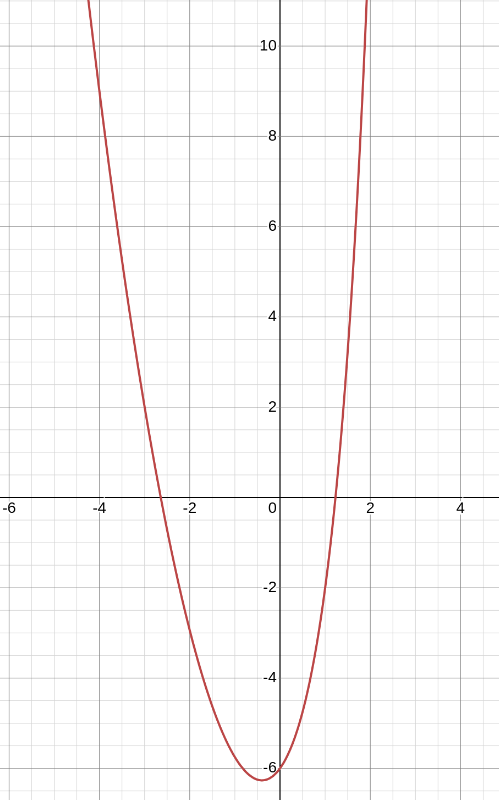
\includegraphics[scale=0.5]{ ./figures/1.png }
    % \end{center}
    \bigbreak \noindent 
    \textit{Then we will use 2 different $x_1$, at -3 and 3}

    \bigbreak \noindent \bigbreak \noindent 
    \subsection{Antiderivitates}
    \begin{itemize}
      \item Know what it means to be an Antiderivitate and how to find them
      \item know the most common Antiderivitates
      \item understand +C
      \item know why 
        \begin{align*}
          x^{\frac{1}{3}} \\ 
          = \frac{3}{4}x^{\frac{4}{3}}
        .\end{align*}
      \item and 
        \begin{align*}
          2y^{2} \\
          = \frac{2}{3}y^{3}
        .\end{align*}
      \item Know that \begin{align*}
        x^{-1} \\
        = \ln{\abs{x}}
      .\end{align*}
    \end{itemize}
     \bigbreak \noindent \bigbreak \noindent
     Common Antiderivitates:
     \bigbreak \noindent 
     \begin{itemize}
      \item Exponential      
    \begin{itemize}
      \item $x^{n} = \frac{x^{n+1}}{n+1} + C$
      \item $\frac{1}{x} = \ln{\abs{x}} + C$
      \item $a^{x} = \frac{a^{x}}{\ln{a}} + C$
      \item $\ln{x} = x\ln{x} - x + C$
      \item $e^{x} = e^{x} + C$
    \end{itemize}
    \bigbreak \noindent \bigbreak \noindent
  \item Trig:
    \begin{itemize}
      \item $\sin{x} = -\cos{x} +  C$
      \item $\cos{x} = \sin{x} + C$
      \item $\tan{x} = \ln{\abs{\sec{x}}} + C$
      \item $\csc{x} = \ln{\abs{\csc{x}-\cot{x}}} + C $
      \item $\sec{x}  = \ln{\abs{\sec{x}+\tan{x}}} + C$
      \item $\cot{x} = \ln{\abs{\sin{x}}} + C$
      \item $\sin^{2}{x} = \frac{1}{2}x-\frac{1}{4}\sin{2x} + C$
      \item $\cos^{2}{x}= \frac{1}{2}x+\frac{1}{4}\sin{2x} + C$
      \item $\tan^{2}{x}= -x + \tan{x} + C $
      \item $\csc^{2}{x}= -\cot{x} + C$
      \item $\sec^{2}{x} =\tan{x} + C$
      \item $\cot^{2}{x} =-x  - \cot{x} + C$
    \end{itemize}
    \bigbreak \noindent \bigbreak \noindent
  \item Hyperbolic Trig
    \begin{itemize}
      \item $\sinh{x} = \cosh{x} + C$
      \item $\cosh{x} = \sinh{x} + C$ 
      \item $\tanh{x} = \ln{\abs{\cos{x}}} + C$
      \item $csch{x} =  \ln{\abs{\tan{h}(\frac{1}{2}x)}} + C$ 
      \item $sech{x} = \tan^{-1}{(\sinh{(x)})} + C$
      \item $coth{x}= \ln{\abs{\sinh{x}}} + C $
      \item $csch^{2}{x} = -\coth{x}+ C$
      \item $sech^{2}{x} = \tanh{x} + C$
    \end{itemize}
    \end{itemize}


    \bigbreak \noindent \bigbreak \noindent 
    \subsection{derivative of hyperbolic trig fuctions}
    \begin{itemize}
      \item $\sinh{x}$ = $\cosh{x} $
      \item $\cosh{x}$ = $\sinh{x} $
      \item $\tanh{x} = \  $sech$^{2}$$x $
      \item sech $x $ = \ -sech $x$ $\tanh{x} $
      \item csch $x$ = \ -csch $x$ $\coth{x}$
      \item $\coth{x}$ = -csch$^{2}x$
    \end{itemize}
    \bigbreak \noindent 
    \textbf{lnx}
    \begin{itemize}
      \item when you have f(x) like:
        \begin{align*}
          f(x) = 3x^{-2}-7x^{-1}+6
        .\end{align*}
        \bigbreak \noindent 
        \textit{you can see if we tried to find F(x), by adding 1 to -1, we would get:}
        \begin{align*}
          \frac{-7^{0}}{0}
        .\end{align*}
        \bigbreak \noindent 
        \textit{Which is a problem, so instead, the Antiderivitive would be $-7\ln{\abs{x}}$}, this is because
        \begin{align*}
          \frac{d}{dx} -7\ln{x}\\ = -\frac{7}{x}
        .\end{align*}
        \bigbreak \noindent 
        \textit{And don't forget the absolute value bars}
    \end{itemize}

    \bigbreak \noindent \bigbreak \noindent
    \subsection{Sigma notation}
    \bigbreak \noindent 
    \begin{itemize}
      \item Know properties of summation:
      \begin{itemize}
           \item $\summation{n}{i=m}c \cdot a_i = c\summation{n}{i=m} a_{i}$, where c is a constant
          \item $\summation{n}{i=m} (a_{i} + b_{i})= \summation{n}{i=m} a_{i} + \summation{n}{i=m} b_{i} $
          \item $\summation{n}{i=m} (a_{i} - b_{i})= \summation{n}{i=m} a_{i} - \summation{n}{i=m} b_{i} $
          \item $\summation{n}{i=1} 1=n $
          \item $\summation{n}{i=1} c=c \cdot n $, where c is a constant
          \item $\summation{n}{i=1} i= \frac{n(n+1)}{2} $
          \item $\summation{n}{i=1}i^{2} = \frac{n(n+1)(2n+1)}{6} $
          \item $\summation{n}{i=1}i^{3}=\bigg[\frac{n(n+1)}{2}\bigg]^{2} $
      \end{itemize}
      \item Know what is means to be a telescoping sum and how to evaluate it.
      \item Know how to eval limits of summation, recall that if you have the limit as n -$>$ infinty, of a rational function whos degress are equal, evaluate the limit
        by taking the ration of the leading coefficients.
    \end{itemize}

    \bigbreak \noindent \bigbreak \noindent 
    \subsection{Area and Distance Problem}
    \begin{itemize}
      \item Know the definition for the area under the curve. 
    \end{itemize}
         \begin{align*}
       A = \lim_{n \to \infty}{R_{n}} = \lim_{n \to \infty}{[\Delta xf(x_{1}) + \Delta xf(x_{2}) + ... + \Delta xf(x_{n})]}
     .\end{align*}
     \begin{center}
       or
     \end{center}
      \begin{align*}
       A = \lim_{n \to \infty}{L_{n}} = \lim_{n \to \infty}{[\Delta xf(x_{0}) + \Delta xf(x_{1}) + ... + \Delta xf(x_{n-1})]}
     .\end{align*}
     \begin{center}
       or
     \end{center}
     \begin{align*}
       A = \lim_{n \to \infty}{[\Delta xf(x_{1}^{*}) + ... + \Delta xf(x_{n}^{*})]}
     .\end{align*}
     \bigbreak \noindent 
     Where $x_{i}^{*}$ is any number in the $i$th interval.
     \nt{$\Delta x =$ Base of each rectangle
       \bigbreak \noindent 
       Find $\Delta x$ with $\frac{b-a}{n}$, on [a,b]
     }
     \bigbreak \noindent 
     \begin{itemize}
       \item And the sigma versions:
     \end{itemize}
      \begin{itemize}
       \item $A = \lim\limits_{n \to \infty}{\summation{n}{i=1}\ \ \Delta xf(x_{i})} $ (Right endpoints)
       \item $A = \lim\limits_{n \to \infty}{\summation{n}{i=1}\ \ \Delta xf(x_{i-1})} $ (Left endpoints)
       \item $A = \lim\limits_{n \to \infty}{\summation{n}{i=1}\ \ \Delta xf(x_{i}^{*})} $ (Arbitrary partiton)
     \end{itemize}

     \bigbreak \noindent 
     \nt{The one with the star denotes not using left or right endpoints}
     \bigbreak \noindent 
     \begin{itemize}
       \item Know how to find $\Delta x$
         \begin{align*}
           \Delta x = \frac{b-a}{n}
         .\end{align*}
        \item Know how to find $x_i$ (right endpoints)
          \begin{align*}
            x_{i} = a + i \Delta x
          .\end{align*}
        \item Know how to find area with a fixed number of rectangles.
          \begin{itemize}
            \item Find $\Delta x $
            \item multiply $\Delta x$ by the sum of all the heights of the rectangles.
          \end{itemize}
     \end{itemize}
     \bigbreak \noindent \bigbreak \noindent
     Notes for riemann sum:
     \begin{itemize}
       \item Say we are using right endpoints with $n=4$, imagine we had the number line:
      \begin{figure}[ht]
          \centering
          \incfig{nlinettt}
          \label{fig:nlinettt}
      \end{figure}
      \begin{itemize}
        \item Since we are using right endpoints with $n=4$, we only use $\frac{5}{4}$ onward
        \item If we were using left endpoints, we would use $1$ to $\frac{7}{2}$
      \end{itemize}
       \end{itemize}


     \bigbreak \noindent \bigbreak \noindent 
     \subsection{Definite Integrals}
      \begin{itemize}
        \item Know: 
          \begin{align*}
            \int_{a}^{b}f(x)dx = \lim\limits_{n \to \infty}{\summation{n}{i=1}\ \ \Delta xf(x_{i}^{*})}
          .\end{align*}
        \item Know riemann sum:
          \begin{align*}
            \summation{n}{i=1}\ \ \Delta xf(x_{i})
          .\end{align*}
        \item Know the properties of integrals:
          \begin{itemize}
            \item $\int_{a}^{b} cdx = c(b-a) $ 
            \item $\int_{a}^{b}cf(x)dx = c \cdot \int_{a}^{b}f(x)dx $
            \item $\int_{a}^{b}[f(x) + g(x)]dx = \int_{a}^{b}f(x)dx + \int_{a}^{b}g(x)dx$
            \item $\int_{a}^{b}[f(x) - g(x)]dx = \int_{a}^{b}f(x)dx - \int_{a}^{b}g(x)dx$
            \item $\int_{a}^{c}f(x)dx = \int_{a}^{b}f(x)dx + \int_{b}^{c}f(x)dx $
            \item if $f(x) \geq 0$ for all $a \leq x \leq b$, then $\int_{a}^{b}f(x)dx \geq  0 $
            \item if $f(x) \geq g(x) $ for all $a \leq x \leq b$, then $\int_{a}^{b}f(x)dx \geq \int_{a}^{b}g(x)dx $
            \item if $m \leq f(x) \leq M $ for $a \leq x \leq b$, then $m(b-a) \leq \int_{a}^{b}f(x)dx \leq M(b-a)$
          \end{itemize}
          \bigbreak \noindent 
        \item Know how to find midpoints
          \begin{itemize}
            \item Make number line with right endpoints, then find the middle value of each interval
            \item If given an interval say, [1,3], and your asked to find midpoints, first plot number line with right endpoints. Then divide $\Delta x$ by 2 and add this number to each left point. Note that $\Delta x$ will remain the same when you find the riemann sum.
          \end{itemize}
        \item Know when you have equations for geometric shapes (circle, half cirle, line)
          \bigbreak \noindent 
        \item integral with the same bounds is \textbf{zero}
        \item Know how to split up integrals like
          \begin{align*}
            \int_{-1}^{2}\ (x-8\abs{x})\ dx
          .\end{align*}
          \begin{itemize}
            \item Set up piecewise
          \end{itemize}
          \begin{align*}
            x= 0\ \text{*Set whats inside abs = 0 to see where sign flips}
          .\end{align*}
               \begin{equation}
                =
                    \begin{cases}
                        x & \text{if } x \geq 0 \\
                        -x & \text{if } x < 0 
                    \end{cases}
                \end{equation}
              \item split integral
                \begin{align*}
                  \int_{-1}^{0}\ x-8(-x)\ dx + \int_{0}^{2}\ x-8x\ dx
                .\end{align*}
              \item Then evaluate
      \end{itemize}

      \bigbreak \noindent \bigbreak \noindent 
      \subsection{The Fundemental theorem of calculus}
      \begin{itemize}
        \item Know
          \begin{align*}
            Part\ 1:\ \frac{d}{dx}\int_{a}^{x}\ f(x)\ dt  = f(x), a \leq x \leq b         \\
            Part\ 2:\ \int_{a}^{b}\ f(x)\ dx = F(b) - F(a)\ where\ F^{\prime} = f. \\
            and \\
            \int_{a}^{b}\ f(x)\ dx = -\int_{b}^{a}\ f(x)\ dx
        .\end{align*}
        \smallbreak \noindent
        \item Know that you have to multiply by the derivative of the upper limit when you substitute for part 1
        \item Know how to split up integrals asked to find the derivative and if given something like:
          \begin{align*}
            F(x) = \int_{x}^{x^{2}}\ e^{t^{7}}\ dx
          .\end{align*}
          \begin{itemize}
            \item so this would end up
              \begin{align*}
                F^{\prime}(x) = \frac{d}{dx}\int_{x}^{0}\ e^{t^{7}}\ dt + \frac{d}{dx}\int_{0}^{x^{2}}\ e^{t^{7}}\ dt
              .\end{align*}
            \item and we would have to flip our limits of integration such that our upper limit is a function of x
              \begin{align*}
                F^{\prime}(x) = \frac{d}{dx}-\int_{0}^{x}\ e^{t^{7}}\ dt + \frac{d}{dx}\int_{0}^{x^{2}}\ e^{t^{7}}\ dt \\
                F^{\prime}(x) = e^{x^{7}} + e^{14} \cdot 2x \\
                 = e^{x^{7}} + 2xe^{14}\\
              .\end{align*}
          \end{itemize}
        \smallbreak \noindent
      \item Know the notation
        \begin{itemize}
          \item If given:
            \begin{align*}
              g(x) = \int_{0}^{x}\ \sqrt{t^{3} + t^{5}}\ dt
            .\end{align*}
          \item Notation for $g^{\prime}$ (using part 1) would be:
            \begin{align*}
              g^{\prime}(x) = \frac{d}{dx}\ \int_{0}^{x}\ \sqrt{t^{3} + t^{5}}\ dt \\
              = \sqrt{x^{3} + x^{5}}
            .\end{align*}
          \item definite integrals do not get +C
        \end{itemize}
      \end{itemize}

      \bigbreak \noindent \bigbreak \noindent 
      \subsection{Indefinite Integrals}
      \begin{itemize}
        \item  Indefinite Integrals are essentially just asking for the Antiderivitate, do not forget +C
        \item review common Antiderivitates
        \item know how to indeterminate antiderivative for inverse trig
        \item Know this antiderivative:
          \begin{align*}
            F(x) = 5^{x} \\
            f(x) = \frac{5^{x}}{\ln{5}} 
          .\end{align*}
          \begin{center}
            Because:
          \end{center}
          \begin{align*}
            \frac{d}{dx}\frac{5^{x}}{\ln{5}} \\
            =\frac{1}{\ln{5}}\bigg[5^{x}\bigg] \\
            = \frac{1}{\ln{5}} \bigg[5^{x} \cdot \ln{5}\bigg] \\
            = \frac{5^{x} \cdot \ln{5}}{\ln{5}} \\
            \boxed{= 5^{x}}
          .\end{align*}
      \end{itemize}

      \bigbreak \noindent \bigbreak \noindent
      \subsection{Velocity Functions with integrals}
      \bigbreak \noindent 
      If given:
      \begin{align*}
        v(t) = 3t-8,\ 0 \leq t \leq 3
      .\end{align*}
      \begin{itemize}
        \item Know that to find displacement: 
          \begin{align*}
            \int_{0}^{3}\ 3t-8\ dt
          .\end{align*}
        \item To find distance traveled:
          \begin{align*}
            \int_{0}^{3}\ \abs{3t-8}\ dx
          .\end{align*}
          \begin{itemize}
            \item So you must write as piecewise and split up the integral (add them)
          \end{itemize}
      \end{itemize}

      \pagebreak \bigbreak \noindent
      \subsection{The Substitution Rule (u-sub)}
      \bigbreak \noindent \bigbreak \noindent
      If $u=g(x)$ is differentiable and its range $\in I $ and $f $ is continuous on $I$, then
      \begin{align*}
        \int f(g(x))g^{\prime}(x)\ dx = \int f(u)\ du
      .\end{align*}
      \bigbreak \noindent \bigbreak \noindent
      \textbf{\textit{\underline{Process:}}}
      \begin{enumerate}
        \item Make a decent choice of what to let u equal
        \item Change our integral from being in terms of $x$, to in terms of $u$
        \item Integrate $\int f(u)\ du $
        \item Change back to $x$
      \end{enumerate}
      \bigbreak \noindent \bigbreak \noindent
      \nt{Also include the constant in your u sub, if it is attached to the function you let u equal,
        Also note for rational trig functions, you can move trig functions from upstairs or downstairs based on their reciprical function, for example, a $\cos^{2}{x}$ in the denominator can be
        moved upstairs as $\sec^{2}{x}$
      }
      \bigbreak \noindent \bigbreak \noindent
      \textbf{\textit{\underline{Notes:}}}
      \begin{itemize}
       \item Our goal with u-sub is to let u equal some function in our composition of functions, such that if we derive that function, we get back something that is also in our integrand
        \item Say we have something like:
          \begin{align*}
            \int \sec^{2}{\theta }\ d\theta  \\ 
            Let\ u = 8\theta  \\
            du = 8d\theta  \\
            \frac{1}{8}du = d\theta 
          .\end{align*}
        \item Know that you can rewrite equations like:
          \begin{align*}
            \int \frac{(\ln{x})^{36}}{x}\ dx \\
            as: \int \frac{1}{x}(\ln{x})^{36}\ dx
          .\end{align*}
        \item Say we have:
          \begin{align*}
            -\frac{1}{2} \int_{0}^{-1}\ e^{u}\ du
          .\end{align*}
          \begin{itemize}
            \item We can flip the limits of integration to remove the negative sign. So we will have:
          \end{itemize}
            \begin{align*}
              \frac{1}{2}\int_{-1}^{0}\ e^{u}\ du
            .\end{align*}
          \item Look out for being able to turn antiderivative into inverse trig functions.
            \begin{itemize}
              \item Say we have:
            \begin{align*}
              \int \frac{x^{7}}{1+x^{16}}\ dx
            .\end{align*}
          \item Don't let $u=1+x^{8} $, we could do this by turning $x^{16}\ into\ (x^{8})^{2}$, but instead, just let $u=x^{8}$. We do this because it ends up like:
            \begin{align*}
             \frac{1}{8}du = x^{7}dx  
            .\end{align*}
          \item So when we sub we get that nice arctan antiderivative, just something to look out for.
            \begin{align*}
              \frac{1}{8}\int \frac{1}{1+u^{2}}\ du
            .\end{align*}
            \end{itemize}
          \item Note that we can write:
            \begin{align*}
              e^{2x}
            .\end{align*}
            \begin{itemize}
              \item as 
            \end{itemize}
            \begin{align*}
              (e^{x})^{2}
            .\end{align*}
      \end{itemize}

      \bigbreak \noindent \bigbreak \noindent
       \textbf{\textit{\underline{Definite Integrals with u-sub}}} 
      \begin{enumerate}
        \item Find what u is going to equal
        \item Find u(a) and u(b) 
        \item make u-sub and use u(a) and u(b) as limits of integration
        \item find antiderivative and evaluate at new limits
      \end{enumerate}
      \bigbreak \noindent 
      \nt{For definite integrals, don't sub back in for u, just evalute integral with u still subbed}


      \pagebreak \bigbreak \noindent
      \subsection{Integrals of Symmetric functions:}
      \bigbreak \noindent \bigbreak \noindent
      \textbf{Sometimes you will run into integrals that are either impossible, or too difficult with u Substitution. For these cases we will look at Integrals of Symmetric Functions}
      \bigbreak \noindent \bigbreak \noindent
      \textbf{\textit{\underline{Even:}}} 
      \begin{align*}
        f(-x)  = f(x)\ then\ \int_{-a}^{a}\ f(x)\ dx  = 2 \int_{0}^{a}\ f(x)\ dx
      .\end{align*}
      \bigbreak \noindent \bigbreak \noindent
      \textbf{\textit{\underline{Odd:}}}
      \begin{align*}
        f(-x) = -f(x)\ then\ \int_{-a}^{a}\ f(x)\ dx = 0
      .\end{align*}

      \bigbreak \noindent \bigbreak \noindent
      \textbf{\textit{\underline{Notes:}}}
      \begin{itemize}
        \item If a function is even, you can replace your lower limit with zero and multiply the integral by 2
        \item if a function is odd, then the integral equals zero.
      \end{itemize}

      \bigbreak \noindent \bigbreak \noindent
      \textbf{\textit{\underline{Figures:}}}
      \begin{figure}[ht]
          \centering
          \incfig{fig1even}
          \incfig{fig2even}
          \label{fig:fig1even}
      \end{figure}

      \pagebreak \bigbreak \noindent
      \begin{center}
        \section{Intro Statistics}
      \end{center}
      \line(1,0){490}
      \bigbreak \noindent 
      \phantomsection
      \addcontentsline{toc}{subsection}{Chapters 1-4}
      \subsection*{Chapters 1-4}
      \bigbreak \noindent 
      \begin{large}
        \textbf{Titles}
      \end{large}
      \bigbreak \noindent 
      \textbf{Chapter 1:}
        \begin{itemize}
          \item 1.1: Introduction to the Practice of Statistics
          \item 1.2: Observational Studies versus Designed Experiments
          \item 1.3: Simple Random Sampling
          \item 1.4: Other Effective Sampling Methods
          \item 1.5: Bias in Sampling
          \item 1.6: The Design of Experiments
        \end{itemize}
      \textbf{Chapter 2:}
        \begin{itemize}
          \item 2.1: Organizing Qualitative Data
          \item 2.2: Organizing Quantitative Data: The Popular Displays
          \item 2.4: Graphical Misrepresentations of Data
        \end{itemize}
      \textbf{Chapter 3:}
        \begin{itemize}
          \item 3.1: Measures of Central Tendency
          \item 3.2: Measures of Dispersion
          \item 3.3: Measures of Central Tendency and Dispersion from Grouped Data
          \item 3.4: Measures of Position
          \item 3.5: The Five-Number Summary and Boxplots
        \end{itemize}
      \textbf{Chapter 4:}
        \begin{itemize}
          \item 4.1: Scatter Diagrams and Correlation
          \item 4.2: Least-Squares Regression
          \item 4.3: Diagnostics on the Least-Squares Regression Line
          \item 4.4: Contingency Tables and Association
        \end{itemize}

        \pagebreak \bigbreak \noindent
        \begin{large}
          \textbf{Learning Objectives}
        \end{large}
        % \addcontentsline{toc}{subsubsection}{Learning Objectives}
        \bigbreak \noindent 
        \begin{itemize}
        \item \textbf{Obtain a simple random sample}
            \item \textbf{Explain the Sources of Bias in Sampling}
            \item \textbf{Describe the Characteristics of an Experiment (vocab)}
            \item \textbf{Explain the Steps in Designing an Experiment}
            \item \textbf{Explain the Completely Randomized Design}
            \item \textbf{Explain the Matched-Pairs Design}
            \item \textbf{Organize Qualitative Data in Tables}
            \item \textbf{Construct Bar Graphs}
            \item \textbf{Construct Pie Charts}
            \item \textbf{Organize Discrete Data in Tables}
            \item \textbf{Construct Histograms of Discrete Data}
            \item \textbf{Organize Continuous Data in Tables}
            \item \textbf{Construct Histograms of Continuous Data}
            \item \textbf{Draw Dot Plots}
            \item \textbf{Identify the Shape of a Distribution}
            \item \textbf{Describe What Can Make a Graph Misleading or Deceptive}
            \item \textbf{Determine the Arithmetic Mean of a Variable from Raw Data}
            \item \textbf{Determine the Median of a Variable from Raw Data}
            \item \textbf{Explain What It Means for a Statistic to be Resistant}
            \item \textbf{Determine the Mode of a Variable from Raw Data}
            \item \textbf{Determine the Range of a Variable from Raw Data}
            \item \textbf{Determine the Standard Deviation of a Variable from Raw Data}
            \item \textbf{Determine the Variance of a Variable from Raw Data}
            \item \textbf{Use the Empirical Rule to Describe Data That Are Bell-Shaped}
           \item \textbf{Approximate the Mean of a Variable from Grouped Data}
           \item \textbf{Compute the Weighted Mean}
           \item \textbf{Approximate the Standard Deviation from a Frequency Distribution}
           \item \textbf{Determine and Interpret z-Scores}
           \item \textbf{Interpret Percentiles}
           \item \textbf{Determine and Interpret Quartiles}
           \item \textbf{Determine and Interpret the Interquartile Range}
           \item \textbf{Check a Set of Data for Outliers}
            \item \textbf{Determine the Five-Number Summary}
            \item \textbf{Draw and Interpret Boxplots}
            \item \textbf{Draw and Interpret Scatter Diagrams}
            \item \textbf{Describe the Properties of the Linear Correlation Coefficient}
            \item \textbf{Compute and Interpret the Linear Correlation Coefficient}
            \item \textbf{4Determine Whether a Linear Relation Exists between Two Variables}
            \item \textbf{Explain the Difference between Correlation and Causation}
            \item \textbf{Find the Least-Squares Regression Line and Use the Line to Make Predictions}
            \item \textbf{Interpret the Slope and the y-Intercept of the Least-Squares Regression Line}
            \item \textbf{Compute the Sum of Squared Residuals}
            \item \textbf{Compute and Interpret the Coefficient of Determination}
            \item \textbf{Perform Residual Analysis on a Regression Model}
            \item \textbf{Identify Influential Observations}
            \item \textbf{Compute the Marginal Distribution of a Variable}
            \item \textbf{Use the Conditional Distribution to Identify Association Among Categorical Data}
            \item \textbf{Explain Simpson's Paradox}
        \end{itemize}


        \pagebreak \bigbreak \noindent
      \begin{large}
        \textbf{Vocab}
      \end{large}
      % \addcontentsline{toc}{subsubsection}{Vocab}
    \begin{itemize}
        \item \textbf{Population:} The entire group to be studied is called the population.
        \item \textbf{Sample:} In statistics, it is often impractical or impossible to get access to the entire \textbf{population}, which is why we only look at a \textbf{sample.} A sample is a \textbf{subset} of the population being studied.
        \item \textbf{Individual:} An individual is a person or object that is a member of the population being studied.
        \item \textbf{Statistic:} A statistic is a numerical summary of a sample.
        \item \textbf{Descriptive Statistics:} Descriptive statistics consist of organizing and summarizing data. Descriptive statistics describe data through numerical summaries, tables, and graphs.
        \item \textbf{Inferential Statistics:} inferential Statistics uses methods that take a result from a sample, extend it to the population, and measure the reliability of the result.
        \item \textbf{Parameter:} A parameter is a numerical summary of a population.
        \item \textbf{Variables:} The characteristics of the individuals in a study. Variables vary, which means they can take on different values.
        \item \textbf{Constants:} Variables that do not vary. Inferential statistics is not necessary with constants.
        \item \textbf{Qualitative, or categorical variables} allow for the classification of individuals base on some attribute or characteristic.
        \item \textbf{Quantitative variables} provide numerical measures of individuals. The values of a quantitative variable can be added or subtracted and provide meaningful results.
        \item A \textbf{discrete variable} is a quantitative variable that has either a finite number of possible values or a countable number of possible values. A discrete variable cannot take on every possible value between any two possible values.
        \item A \textbf{continuous variable} is a quantitative variable that has an infinite number of possible values that are not countable. A continuous variable may take on every possible value between any two values. Continuous variables typically result from measurement. Continuous variables are often rounded. If a certain make of car gets 24 miles per gallon (mpg) of gasoline, its miles per gallon must be greater than or equal to 23.5 and less than 24.5, or $23.5 \leq mpg \leq 24.5$
        \item The list of observed values for a variable is \textbf{data.}
        \item \textbf{Qualitative data} are observations corresponding to a \textbf{qualitative variable.}
        \item \textbf{Quantitative data} are observations corresponding to a quantitative variable.
        \item \textbf{Discrete data} are observations corresponding to a discrete variable.
        \item \textbf{Continuous data} are observations corresponding to a continuous variable.
            \item \textbf{Explanatory Variable:} An explanatory variable, also known as an independent variable or predictor variable, is a variable that is manipulated or controlled by researchers in an experiment or study. It is the variable that is hypothesized to have an impact on the outcome or dependent variable. 
            \item \textbf{Lurking variable}: An explanatory variable that was not considered in a study, but that affects the value of the response variable.
            \item \textbf{Response Variable}: The response variable, also known as the dependent variable or outcome variable, is the variable that is measured or observed to determine the effect or response of the explanatory variable(s). It is the variable that researchers are interested in studying or predicting. 
            \item \textbf{Confounding:} Occurs when the effects of two or more explanatory variables are not separated. Therefore, any relation that may exist between an explanatory variable and the response variable may be due to some other variable or variables not accounted for in the study.
            \item \textbf{Census:} List of individuals in a population along with certain characteristics of each individual.
            \item \textbf{Random Sampling:} The process of using chance to select individuals from a population to be included in the sample.
            \item \textbf{Simple Random Sampling:} A sample of size $n$  from a population of size $N $  is obtained through simple random sampling if every possible sample of size $n$  has an equal chance of occurring. The sample is then called a simple random sample.
                \begin{itemize}
                    \item $n < N $
                \end{itemize}
            \item \textbf{frame:} a list of all the individuals within the population.
            \item \textbf{Sample Without Replacement:} Once an individual is selected, the individual cannot be selected again.
            \item \textbf{Stratified sample}: is obtained by dividing the population into nonoverlapping groups called strata and then obtaining a simple random sample from each stratum. The individuals within each stratum should be homogenous (similar) in some way.
                \begin{itemize}
                    \item Within Stratified samples, the number of individuals sampled from each stratum should be proportional to the size of the strata in the population.
                \end{itemize}
            \item \textbf{Systematic sample} is obtained by selecting every $k$th individual from the population. The first individual selected corresponds to a number between 1 and $k$
            \item \textbf{Cluster sample} is obtained by selecting all individuals within a randomly selected collection or group of individuals.
            \item \textbf{Convenience sample:} the individuals are easily obtained and not based on randomness.
            \item \textbf{Bias:} If the results of the sample are not representative of the population. Sampling bias means that the technique used to obtain the sample's individuals tends to favor one part of the  population over another. Any convenience sample has sampling bias because the individuals are not chosen through a random sample.
            \item \textbf{Undercoverage:} Occurs when the proportion of one segment of the population is lower in a sample than it is in the population. This can result if the frame used to obtain the sample is incomplete or not representative of the population.
            \item \textbf{Sampling bias:} sampling bias is a bias in which a sample is collected in such a way that some members of the intended population have a lower or higher sampling probability than others. It results in a biased sample of a population in which all individuals, or instances, were not equally likely to have been selected
            \item \textbf{Nonresponse bias:} exists when individuals selected to be in the sample who do not respond to the survey have different opinions from those who do
                \begin{itemize}
                    \item This can be controlled with \textbf{callbacks}.
                    \item This can also be controlled with \textbf{rewards or incentives}
                \end{itemize}
            \item \textbf{Response bias:} Exists when the answers on a survey do not reflect the true feelings of the respondent.
            \item \textbf{Open Question:} Allows the respondent to choose his or her response
            \item \textbf{Closed Question:} requires the respondent to choose from a list of predetermined responses
            \item \textbf{Nonsampling errors:} result from undercoverage, nonresponse bias, response bias, or data-entry error. Such errors could also be present in a census.
            \item \textbf{Sampling error:} results from using a sample to estimate information about a population. This type of error occurs because a sample gives incomplete information about a population.
            \item \textbf{Experiment:} is a controlled study conducted to determine the effect of varying one or more explanatory variables or \textbf{factors} has on a response variable. 
            \item \textbf{Factor:} A variable whose effect on the response variable is to be assessed by the experimenter
            \item \textbf{Treatment:} Any combination of the values of the factors is called a treatment
            \item \textbf{Experimental Unit (or subject)} is a person, object or some other well-defined item upon which a treatment is applied
            \item \textbf{Control Group:} Serves as a baseline treatment that can be used to compare to other treatments.
            \item \textbf{Placebo:} is an innocuous medication, such as a sugar tablet, that looks, tastes, and smells like the experimental medication.
            \item \textbf{Blinding:} refers to nondisclosure of the treatment an experimental unit is receiving.
            \item \textbf{Single-blind} experiment is one in which the experimental unit (or subject) does not know which treatment he or she is receiving.
            \item \textbf{Double-blind} experiment is one in which neither the experimental unit nor the researcher in contact with the experimental unit knows which treatment the experimental unit is receiving.
            \item \textbf{Design:} To design an experiment means to describe the overall plan in conducting the experiment. Conducting an experiment requires a series of steps.
            \item \textbf{Blocking:} Grouping together similar experimental units and then randomly assigning the experimental units within each group to a treatment is called 
            \item \textbf{completely randomized design:} is one in which each experimental unit is randomly assigned to a treatment.
            \item \textbf{matched-pairs design:} is an experimental design in which the experimental units are paired up. The pairs are selected so that they are related in some way (that is, the same person before and after a treatment, twins, husband and wife, same geographical location, and so on). There are only two levels of treatment in a matched-pairs design.
            \item \textbf{The relative frequency} is the proportion (or percent) of observations within a category and is found using the formula
            \item \textbf{Classes: } The Categories in which data is grouped
            \item \textbf{lower class limit:} the smallest value within the class 
            \item \textbf{upper class limit:} the largest value within the class 
            \item \textbf{Class Width: }  is the difference between consecutive lower class limits.
            \item A table is \textbf{open ended} if the first class has no lower class limit or the last class has no upper class limit
            \item \textbf{uniform distribution:} frequency of each value of the variable is evenly spread across the values of the variable. 
            \item \textbf{bell-shaped distribution:} highest frequency occurs in the middle and frequencies tail off to the left and right of the middle.
            \item \textbf{skewed right:} the tail to the right of the peak is longer than the tail to the left of the peak
            \item \textbf{skewed left:} tail to the left of the peak is longer than the tail to the right of the peak.
            \item \textbf{The arithmetic mean} of a variable is computed by adding all the values of the variable in the data set and dividing by the number of observations.
            \item \textbf{The population arithmetic mean}, $\mu$, (pronounced "mew"), is a parameter that is computed using data from all the individuals in a population.
            \item \textbf{The sample arithmetic mean}, $\bar{x}$ (pronounced x-bar"), is a statistic that is computed using data from individuals in a sample.
            \item \textbf{The median} of a variable is the value that lies in the middle of the data when arranged in ascending order. We use $M$  to represent the median.
            \item A numerical summary of data is said to be \textbf{resistant} if observations that are extreme (very large or small) relative to the data do not affect its value substantially.
                \begin{itemize}
                    \item So the median is resistant, but the mean is not resistant.
                \end{itemize}
            \item \textbf{The mode} of a variable is the observation of the variable that occurs most frequently in the data set.
                \begin{itemize}
                    \item If no observation occurs more than once, we say that the data have \textbf{no mode}.
                \end{itemize}
            \item \textbf{Bimodal:} If the data has two modes
            \item \textbf{Multimodal:} If the data has more than two modes
            \item \textbf{Dispersion:} Degree to which the data are spread out. 
            \item \textbf{Range:} The range, $r $, of a variable is the difference between the largest and smallest data value. That is,
                \textbf{Note:} Range is \textbf{not} resistant
            \item \textbf{Deviation about the mean:} a deviation refers to the difference between an individual data point and a central value, such as the mean or median. It represents how much a particular data point varies or deviates from the average or typical value in a data set. 
                \bigbreak \noindent 
                \textbf{Note:} The sum of the deviations about the mean always equals zero
            % \item \textbf{The population standard deviation} of a variable is the square root of the sum of squared deviations about the population mean divided by the number of observations in the population, $N$. The population standard deviation is symbolically represented by $\sigma$ (lowercase Greek sigma). The formula is given by:
            %     \textbf{Note:} Standard Deviation is \textbf{not} resistant
            % \item \textbf{The sample standard deviation}, $s $, of a variable is the square root of the sum of squared deviations about the sample mean divided by $n-1 $, where $n$  is the sample size. The formula is given as
            %     \textbf{Note:} Standard Deviation is \textbf{not} resistant
              \item \textbf{Standard Deviation:} Measure of dispersion. It gives us a sense of how much the individual values deviate or differ from the average (mean) value. The standard deviation and the mean together can tell you where most of the values in your frequency distribution lie if they follow a normal distribution (Empirical Rule).
            \item  we call $n-1$ the \textbf{degrees of freedom} because the first $n-1 $  observations have freedom to be any value, but the $n^{th}$ observation has no freedom. It must be whatever value forces the sum of the deviations about the mean to equal zero.
            \item The \textbf{variance}  It assesses the average squared difference between data values and the mean. Find my squaring $\sigma $ or $s$ \\
              \textbf{Note:} The units of measure in variance are squared values. So if the variable is measured in dollars, the variance is measured in dollars squared. This makes interpreting the variance difficult.
                \item \textbf{Coefficient of Variation:} The coefficient of​ variation, CV, is defined as the ratio of the standard deviation to the mean of a data set. The CV allows for a comparison in spread by describing the amount of spread per unit mean.
               \textbf{Note:} When converting units of​ measure, the coefficient of variation is unchanged.
             \item \textbf{Class Midpoint:} The class midpoint is the sum of consecutive lower class limits divided by 2
             \item \textbf{Approximate Population Mean (if we do not have access to the original data, ie data has been grouped (classed) and frequency chart has already been made)}
            \item \textbf{Approximate Sample Mean (if we do not have access to the original data, ie data has been grouped (classed) and frequency chart has already been made)}
            \item \textbf{The weighted mean}, $\overline{x}_{w}$, of a variable is found by multiplying each value of the variable by its corresponding weight, adding these products, and dividing this sum by the sum of the weights. It can be expressed using the formula
            \item \textbf{Approximate Population Standard Deviation (if we do not have access to the original data, ie data has been grouped (classed) and frequency chart has already been made)}
            \item \textbf{Approximate Sample Standard Deviation (if we do not have access to the original data, ie data has been grouped (classed) and frequency chart has already been made)}
             \item \textbf{The z-score} represents the distance that a data value is from the mean in terms of the number of standard deviations. We find it by subtracting the mean from the data value and dividing this result by the standard deviation.
                 \textbf{Note:} The Z-score is unitless. It has mean  0 and a standard deviation of 1 \\
                 \textbf{Round z-scores to the nearest hundredth}
             \item  The median is a special case of a general concept called the \textbf{percentile.}
             \item \textbf{the $k^{th}$  percentile,} denoted $P_{k} $,  of a set of data is a value such that $k $  percent of the observations are less than or equal to the value.
                \item The most common percentiles are \textbf{quartiles}, which divide data sets into fourths, or four equal parts.
                \item The \textbf{interquartile range, IQR,} is the range of the middle $50\% $  of the observations in a data set. That is, the IQR is the difference between the first and third quartiles and is found using this formula  
               \item \textbf{Outliers:} When analyzing data, we must check for extreme observations, called outliers. Outliers can occur by chance, because of errors in the measurement of a variable, during data entry, or from errors in sampling.
                \item \textbf{Fences} serve as cutoff points for determining outliers.
        \item \textbf{bivariate data:} data in which two variables are measured on an individual. For example, we might want to know whether the amount of cola consumed per week is related to a person's bone density. The individuals would be the people in the study, and the two variables would be the amount of cola consumed weekly and bone density.
        \item Two variables that are linearly related are \textbf{positively associated} when above-average values of one variable are associated with above-average values of the other variable (or below-average values of one variable are associated with below-average values of the other variable). That is, two variables are positively associated if, whenever the value of one variable increases, the value of the other variable also increases.
        \item Two variables that are linearly related are \textbf{negatively associated} when above-average values of one variable are associated with below-average values of the other variable. That is, two variables are negatively associated if, whenever the value of one variable increases, the value of the other variable decreases.
        \item The \textbf{linear correlation coefficient}, or Pearson product moment correlation coefficient, is a measure of the strength and direction of the linear relation between two quantitative variables. The Greek letter $\rho $ (rho) represents the population correlation coefficient, and $r $ represents the sample correlation coefficient. We present only the formula for the sample correlation coefficient.
        \item \textbf{The least-squares regression line} minimizes the sum of the squared errors (or residuals). This line minimizes the sum of the squared vertical distance between the observed values of $y$  and those predicted by the line, $\hat{y}$  (read “y-hat"). We represent this as $\sum residuals^{2}$
        \item The observed distance for this club-head speed is 274 yards. The difference between the observed and predicted values of y is the error, or \textbf{residual}.
            \begin{align*}
                Residual\ = observed - predicted
            .\end{align*}
        \item \textbf{The coefficient of determination}, $R^{2}$, measures the proportion of total variation in the response variable that is explained by the least-squares regression line.
            \begin{align*}
                R^{2} = r^{2}
            .\end{align*}
        \item \textbf{An influential observation} significantly affects the least-squares regression line's slope and/or y-intercept. (It also affects the value of the correlation coefficient.) Methods exist for determining whether a particular observation is influential; however, they are beyond the scope of this course. Nonetheless, we can still get a sense as to whether a particular observation is influential right now.
        \item the difference in our predicted value, and our actual value, is due to factors (variables) other than the club-head speed (wind speed and position of the ball on the club face, for example) and to random error. The differences just discussed are called \textbf{deviations}.
        \item \textbf{Total Deviation:} The deviation between the observed value, y, and mean value, $\overline{y} $, of the response variable.
            \begin{align*}
                &y - \overline{y} \\
                &Or: \text{Explained Deviation + Unexplained Deviation}
            .\end{align*}
        \item \textbf{Explained Deviation:} The deviation between the predicted value, $\hat{y} $, and mean value, $\overline{y} $, of the response variable.
            \begin{align*}
                \hat{y}-\overline{y}
            .\end{align*}
        \item \textbf{Unexplained Deviation:} The deviation between the observed value, y, and predicted value, $\hat{y} $, of the response variable
            \begin{align*}
                y - \hat{y}
            .\end{align*}
        \item     If a plot of the residuals against the explanatory variable shows the spread of the residuals increasing or decreasing as the explanatory variable increases, then a strict requirement of the linear model is violated.     This requirement is called \textbf{constant error variance}. The statistical term for constant error variance is \textbf{homoscedasticity}

        \item \textbf{Simpson's Paradox}, which describes a situation in which an association between two variables inverts or goes away when a third variable is introduced to the analysis.
        \end{itemize}

        \pagebreak \bigbreak \noindent
        \begin{large}
          \textbf{Charts and Graphs:}
        \end{large}
        \begin{itemize}
           \item \textbf{A frequency distribution} lists each category of data and the number of occurrences for each category of data.
           \item \textbf{A relative frequency distribution} lists each category of data together with the relative frequency.
             \item \textbf{A bar graph} is constructed by labeling each category of data on either the horizontal or vertical axis and the frequency or relative frequency of the category on the other axis. Rectangles of equal width are drawn for each category. The height of each rectangle represents the category's frequency or relative frequency.
            \item \textbf{A Pareto chart} is a bar graph whose bars are drawn in decreasing order of frequency or relative frequency.
            \item \textbf{A pie chart} is a circle divided into sectors. Each sector represents a category of data. The area of each sector is proportional to the frequency of the category.
            \item A \textbf{histogram} is constructed by drawing rectangles for each class of data. The height of each rectangle is the frequency or relative frequency of the class. The width of each rectangle is the same, and the rectangles touch each other.
            \item We draw a \textbf{dot plot} by placing each observation horizontally in increasing order and placing a dot above the observation each time it is observed.
             \item The \textbf{five-number summary} of a set of data consists of the smallest data value, $Q_{1} $  the median, $Q_{3} $  and the largest data value. We use the five-number summary to learn information about the extremes of the data set. The summary is organized as follows:
              \begin{center}
                 Minimum $Q_{1} $ $M$ $Q_{3} $  Maximum
              \end{center}
        \item \textbf{A scatter diagram} is a graph that shows the relationship between two quantitative variables measured on the same individual. Each individual in the data set is represented by a point in the scatter diagram. The explanatory variable is plotted on the horizontal axis, and the response variable is plotted on the vertical axis.
          \begin{itemize}
            \item A scatter plot is useful to determine if the presence of outliers causing an effect.
          \end{itemize}
        \item \textbf{A marginal distribution} of a variable is a frequency or relative frequency distribution of either the row or column variable in the contingency table.
        \item \textbf{A conditional distribution} lists the relative frequency of each category of the response variable, given a specific value of the explanatory variable in the contingency table.
        \end{itemize}


        \pagebreak \bigbreak \noindent
        \begin{large}
          \textbf{Formulas}
        \end{large}
        % \addcontentsline{toc}{subsubsection}{Formulas}
        \bigbreak \noindent 
        \begin{itemize}
                        \item \textbf{The relative frequency} is the proportion (or percent) of observations within a category. 
                \begin{align*}
                    Relative\ frequency = \frac{Frequency}{Sum\ of\ all\ frequency}
                .\end{align*}

                    \item \textbf{The population arithmetic mean}, $\mu$, (pronounced "mew"), is a parameter that is computed using data from all the individuals in a population.
                \begin{align*}
                    \mu = \frac{x_{1}+x_{2} + x_{N}}{N} = \frac{\summation{}{}x_{i}}{N}
                .\end{align*}
            \item \textbf{The sample arithmetic mean}, $\bar{x}$ (pronounced x-bar"), is a statistic that is computed using data from individuals in a sample.
                \begin{align*}
                    \bar{x} = \frac{x_{1}+x_{2} + x_{n}}{n} = \frac{\summation{}{}x_{i}}{n}
                .\end{align*}
            \item \textbf{The median} of a variable is the value that lies in the middle of the data when arranged in ascending order. We use $M$  to represent the median.
                \begin{itemize}
                    \item For odd $n$:
                        \begin{align*}
                            M = \frac{n+1}{2}
                        .\end{align*}
                    \item For even $n$:
                        \begin{align*}
                            M = Average\ of\ \frac{n}{2}, \frac{n}{2}+1
                        .\end{align*}
                \end{itemize}
            \item \textbf{Range:} The range, $r $, of a variable is the difference between the largest and smallest data value. That is,
                \begin{align*}
                    range = R = Largest\ data\ value- smallest\ data\ value
                .\end{align*}
            \item \textbf{Deviation:} a deviation refers to the difference between an individual data point and a central value, such as the mean or median. It represents how much a particular data point varies or deviates from the average or typical value in a data set. When can comopute a deviation with:
                \begin{align*}
                    Individual\ data\ point - mean
                .\end{align*}


            \item \textbf{The population standard deviation} of a variable is the square root of the sum of squared deviations about the population mean divided by the number of observations in the population, $N$. The population standard deviation is symbolically represented by $\sigma$ (lowercase Greek sigma). The formula is given by:
                \begin{align*}
                    \sigma = \sqrt{\frac{(x_{1} - \mu)^{2} + (x_{2}-\mu)^{2}+...+(x_{N}-\mu)^{2}}{N}} \\
                    = \sqrt{\frac{\summation{}{}(x_{i}-\mu)^{2} }{N}}
                .\end{align*}
                \textbf{Note:} Standard Deviation is \textbf{not} resistant
            \item \textbf{The sample standard deviation}, $s $, of a variable is the square root of the sum of squared deviations about the sample mean divided by $n-1 $, where $n$  is the sample size. The formula is given as
                \begin{align*}
                    s = \sqrt{\frac{(x_{1} - \overline{x})^{2}+(x_{2}-\overline{x})^{2}+...+(x_{n}-\overline{x})^{2}}{n-1}}\\
                    = \sqrt{\frac{\summation{}{}(x_{i}-\overline{x})^{2}}{n-1}}
                .\end{align*}
                \textbf{Note:} Standard Deviation is \textbf{not} resistant
            \item  \textbf{The population variance} is \textbf{$\sigma^{2}$} 
            \item \textbf{The Sample Variance} is $s^{2}$
             \item \textbf{Approximate Population Mean (if we do not have access to the original data, ie data has been grouped (classed) and frequency chart has already been made)}
                \begin{align*}
                    \mu =\frac{\sum x_i f_i}{\sum f_i} \\
                     =\frac{x_1 f_1+x_2 f_2+\cdots+x_n f_n}{f_1+f_2+\cdots+f_n}
                .\end{align*}
            where: $\quad x_i$ is the midpoint or value of the $i$ th class  \\
            $f_i$ is the frequency of the $i$ th class  \\
            $n$ is the number of classes
            \item \textbf{Approximate Sample Mean (if we do not have access to the original data, ie data has been grouped (classed) and frequency chart has already been made)}
                \begin{align*}
                    \overline{x} = \frac{\sum x_{i}f_{i}}{\sum f_{i}} \\
                     = \frac{x_{1}f_{1} + x_{2} f_{2} + ... +x_{n} f_{n}}{f_{1} + f_{2} + ... + f_{n}}
                .\end{align*}
            where: $\quad x_i$ is the midpoint or value of the $i$ th class  \\
            $f_i$ is the frequency of the $i$ th class  \\
            $n$ is the number of classes
            \item \textbf{The weighted mean}, $\overline{x}_{w}$, of a variable is found by multiplying each value of the variable by its corresponding weight, adding these products, and dividing this sum by the sum of the weights. It can be expressed using the formula
                \begin{align*}
                    \overline{x}_{w} = \frac{\sum w_{i}x_{i}}{w_{i}} = \frac{w_{1} + x_{1} + w_{2} + x_{2} + ... + w_{n} + x_{n}}{w_{1} + w_{2} + ... + w_{n}}
                .\end{align*}
                Where: \quad $w_{i}$ is the weight of the $i^{th}$ observation \\
                $x_{i}$ is the value of the $i^{th}$ observation.
            \item \textbf{Approximate Population Standard Deviation (if we do not have access to the original data, ie data has been grouped (classed) and frequency chart has already been made)}
                \begin{align*}
                    \sigma = \sqrt{\frac{\sum(x_{i} - \mu)^{2}f_{i}}{\sum f_{i}}}
                .\end{align*}
                Where: \quad  $x_{i}$ is the midpoint or value of the ith class \\
                $f_{i}$ is the frequency of the $i^{th}$ class
            \item \textbf{Approximate Sample Standard Deviation (if we do not have access to the original data, ie data has been grouped (classed) and frequency chart has already been made)}
                \begin{align*}
                    s = \sqrt{\frac{\sum(x_{i}-\overline{x})^{2}f_{i}}{\sum f_{i} -1}}
                .\end{align*}
                Where: \quad  $x_{i}$ is the midpoint or value of the ith class \\
                $f_{i}$ is the frequency of the $i^{th}$ class
             \item \textbf{The z-score} represents the distance that a data value is from the mean in terms of the number of standard deviations. We find it by subtracting the mean from the data value and dividing this result by the standard deviation.
                 \begin{itemize}
                     \item \textbf{Population Z-score}
                 \end{itemize}
                 \begin{align*}
                      z = \frac{x - \mu}{\sigma}
                 .\end{align*}
                 \begin{itemize}
                     \item \textbf{Sample Z-score}
                 \end{itemize}
                 \begin{align*}
                     z =\frac{x-\overline{x}}{s}
                 .\end{align*}
                 \textbf{Note:} The Z-score is unitless. It has mean  0 and a standard deviation of 1 \\
                 \textbf{Round z-scores to the nearest hundredth}
                \item The \textbf{interquartile range, IQR,} is the range of the middle $50\% $  of the observations in a data set. That is, the IQR is the difference between the first and third quartiles and is found using this formula  
                    \begin{align*}
                        IQR = Q_{3} - Q_{1}
                    .\end{align*}
                \item \textbf{Fences} serve as cutoff points for determining outliers.
                    \begin{align*}
                        Lower\ Fence\ = Q_{1} - 1.5\cdot IQR \\
                        Upper\ Fence\ = Q_{3} + 1.5\cdot IQR
                    .\end{align*}
        \item The \textbf{five-number summary} of a set of data consists of the smallest data value, $Q_{1} $  the median, $Q_{3} $  and the largest data value. We use the five-number summary to learn information about the extremes of the data set. The summary is organized as follows:
        \begin{center}
           Minimum $Q_{1} $ $M$ $Q_{3} $  Maximum
        \end{center}
        \item The \textbf{linear correlation coefficient}, or Pearson product moment correlation coefficient, is a measure of the strength and direction of the linear relation between two quantitative variables. The Greek letter $\rho $ (rho) represents the population correlation coefficient, and $r $ represents the sample correlation coefficient. We present only the formula for the sample correlation coefficient.
            \begin{align*}
                r =\frac{\sum\left(\frac{x_i-\bar{x}}{s_x}\right)\left(\frac{y_i-\bar{y}}{s_y}\right)}{n-1}
            .\end{align*}
            Where:
            \bigbreak \noindent 
                $x_i$ is the $i$ th observation of the explanatory variable \\
                $\overline{x}$ is the sample mean of the explanatory variable \\
                $s_{x} $is the sample standard deviation of the explanatory variable \\
                $y_i$ is the $i$ th observation of the response variable \\
                $\overline{y}$ is the sample mean of the response variable \\
                $\mathbf{S}_y$ is the sample standard deviation of the response variable \\
                $n$ is the number of individuals in the sample

        \item \textbf{The least-squares regression line} minimizes the sum of the squared errors (or residuals). This line minimizes the sum of the squared vertical distance between the observed values of $y$  and those predicted by the line, $\hat{y}$  (read “y-hat"). We represent this as $\sum residuals^{2}$
            \begin{align*}
               \hat{y} = b_{1}x + b_{0} 
            .\end{align*}
            Where:
            \begin{align*}
                b_{1} = r \cdot \frac{s_{y}}{s_{x}}\ \text{is the slope of the least-squares regression line}
            .\end{align*}
            And:
            \begin{align*}
                b_{0} = \overline{y} -b_{1}\overline{x}\ \text{is the y-Intercept of the least-squares regression line} 
            .\end{align*}
        \item The observed distance for this club-head speed is 274 yards. The difference between the observed and predicted values of y is the error, or \textbf{residual}.
            \begin{align*}
                Residual\ = observed - predicted
            .\end{align*}
        \item \textbf{The coefficient of determination}, $R^{2}$, measures the proportion of total variation in the response variable that is explained by the least-squares regression line.
            \begin{align*}
                R^{2} = r^{2}
            .\end{align*}

        \item \textbf{Total Deviation:} The deviation between the observed value, y, and mean value, $\overline{y} $, of the response variable.
            \begin{align*}
                &y - \overline{y} \\
                &Or: \text{Explained Deviation + Unexplained Deviation}
            .\end{align*}
        \item \textbf{Explained Deviation:} The deviation between the predicted value, $\hat{y} $, and mean value, $\overline{y} $, of the response variable.
            \begin{align*}
                \hat{y}-\overline{y}
            .\end{align*}
        \item \textbf{Unexplained Deviation:} The deviation between the observed value, y, and predicted value, $\hat{y} $, of the response variable
            \begin{align*}
                y - \hat{y}
            .\end{align*}

        \item \textbf{Empirical Rule}
          \begin{itemize}
             \item approximately $68\% $ of the data within $1 $ standard deviation of the mean. That is, approximately $68\% $  of the data will lie between $\mu-1 \sigma $ and $\mu + 1 \sigma $ 
               \begin{align*}
                 \mu \pm 1\cdot \sigma
               .\end{align*}
             \item approximately $95\% $ of the data within $2 $ standard deviation of the mean. That is, approximately $95\% $  of the data will lie between $\mu-2 \sigma $ and $\mu + 2 \sigma $ 
               \begin{align*}
                 \mu \pm 2 \cdot \sigma
               .\end{align*}
             \item approximately $99.7\% $ of the data within $3 $ standard deviation of the mean. That is, approximately $99.7\% $  of the data will lie between $\mu-3 \sigma $ and $\mu + 3 \sigma $ 
               \begin{align*}
                 \mu \pm 3 \cdot \sigma
               .\end{align*}
           \end{itemize}
        \end{itemize}
          \item \textbf{Coefficient of Variation:}
            \begin{align*}
              \frac{Standard\ Deviation}{Mean}
            .\end{align*}

           \pagebreak \bigbreak \noindent
       \textbf{Deciding Which Measure of Central Tendency and Dispersion to Report:}
       \bigbreak \noindent 
       \begin{center}
           \begin{tabular}{|l|l|l|}
            \hline
            Shape of Distribution & Measure of Central Tendency & Measure of Dispersion \\
            \hline
            Symmetric & Mean & Standard Deviation \\
            \hline
            Skewed Left or Skewed Right & Median & Interquartile Range \\
            \hline
            \end{tabular}
       \end{center}
       \bigbreak \noindent 
       \nt{For the remainder of this course, the phrase "describe the distribution" will mean to describe its shape (skewed left, skewed right, or symmetric), its center (mean or median), and its spread (standard deviation or interquartile range).}

       \bigbreak \noindent 
       \textbf{Resistant Measures of Central Tendency:}
       \begin{itemize}
           \item \textbf{Median}
       \end{itemize}
      \textbf{Non-Resistant Measures of Central Tendency:}
      \begin{itemize}
          \item \textbf{Mean}
          \item \textbf{Mode}
      \end{itemize}
      \bigbreak \noindent 
      \textbf{Resistant Measures of Dispersion:}
      \begin{itemize}
          \item \textbf{Quartiles}
      \end{itemize}
      \bigbreak \noindent 
    \textbf{Non-Resistant Measures of Dispersion:}
    \begin{itemize}
        \item \textbf{Range.}
        \item \textbf{Standard Deviation.}
        \item \textbf{Variance.}
    \end{itemize}

    \pagebreak 
    \phantomsection
    \addcontentsline{toc}{subsection}{5-8 Subsection Titles}
    \subsection*{5-8 Subsection Titles}
    \bigbreak \noindent 
    \textbf{Chapter 5:}
    \begin{itemize}
      \item 5.1: Probability Rules
      \item 5.2: The Addition Rule and Complements
      \item 5.3: Independence and the Multiplication Rule
    \end{itemize}



    \pagebreak 
    \phantomsection
    \addcontentsline{toc}{subsection}{5-8 Vocab}
    \subsection*{5-8 Vocab}
    \bigbreak \noindent 
    \begin{itemize}
        \item \textbf{Simulation:} is a technique used to recreate a random event.
        \item \textbf{Random Process:} represents scenarios where the outcome of any particular trial of an experiment is unknown, but the proportion (or relative frequency) of a particular outcome is observed and approaches a specific value
        \item \textbf{Probability:} Is the measure of the likelihood of a random phenomenon or chance behavior occurring. It deals with experiments that yield random short-term results or outcomes yet reveal long-term predictability. The long-term proportion in which a certain outcome is observed is the probability of that outcome. 
        \item \textbf{Outcomes:} Short term results
        \item \textbf{The Law of Large Numbers:} As the number of repetitions of a probability experiment increases, the proportion with which a certain outcome is observed gets closer to the probability of the outcome.
        \item \textbf{an experiment} is any process with uncertain results that can be repeated.
        \item \textbf{The sample space, $S$,} of a probability experiment is the collection of all possible outcomes for that experiment.
        \item \textbf{An event} is any collection of outcomes from a probability experiment. An event consists of one or more outcomes. We denote events with one outcome, sometimes called simple events, as $e_{i}$. In general, events are denoted using capital letters such as $ E$.
        \item \textbf{A probability model} lists the possible outcomes of a probability experiment and each outcome's probability. A probability model must satisfy Rules 1 and 2 of the rules of probabilities.
        \item  \textbf{An unusual event} is an event that has a low probability of occurring.
        \item An experiment has \textbf{equally likely outcomes} when each outcome has the same probability of occurring. 
        \item A \textbf{subjective probability} is a probability that is determined based on personal judgment.
        \item \textbf{Disjoint:} Two events are disjoint if they have no outcomes in common. 
        \item \textbf{Mutually Exclusive:} Another name for disjoint events.
        \item \textbf{Complement of $E$:} Let $S$ denote the sample space of a probability experiment and let $E$ denote an event. The complement of $E $, denoted $E^{C} $, is all outcomes in the sample space $S $ that are not outcomes in the event $E $.
        \item \textbf{Two events being Independent: } Two events $E$ and $F$ are independent if the occurrence of event $E$ in a probability experiment does not affect the probability of event $F $.
        \item \textbf{Two events being Dependent:} Two events are dependent if the occurrence of event $E $ in a probability experiment affects the probability of event $F$.
    \end{itemize}

    \pagebreak 
    \phantomsection
    \addcontentsline{toc}{subsection}{5-8 Formulas}
    \subsection*{5-8 Formulas}
    \bigbreak \noindent 
        \begin{itemize}
        \item \textbf{Computing probability with the empirical method}
        \begin{align*}
            P(E) = \text{Relative frequency of E} = \frac{Frequency\ of\ E}{number\ of\ trials\ of\ experiment}
        .\end{align*}
      \item \textbf{Computing Probability With The Classical Method}
            \begin{itemize}
                \item If an experiment has n equally likely outcomes and if the number of ways that an event E can occur is m, then the probability of E,P(E), is
            \end{itemize}
            \begin{align*}
                P(E) = \frac{\text{number of ways that $E$ can occur}}{\text{number of possible outcomes}} = \frac{m}{n}
            .\end{align*}
            \begin{itemize}
                \item So, if S is the sample space of this experiment, then
                    \begin{align*}
                        P(E) = \frac{N(E)}{N(E)}
                    .\end{align*}
            where N(E) is the number of outcomes in E, and N(S) is the number of outcomes in the sample space.
            \end{itemize}
                    \item \textbf{Addition Rule for Disjoint Events:}
            \begin{itemize}
                \item if $E $ and $F $ are disjoint (or mutually exclusive) events, then:
                    \begin{align*}
                        P(E\ or\ F) = P(E) + P(F)
                    .\end{align*}
            \end{itemize}
        \item \textbf{Addition Rule for Non-Disjoint Events (General Addition Rule)}
          \begin{align*}
            P(E\ or\ F) = (P(E) + P(F)) - P(E\ and\ F)
          .\end{align*}
        \item \textbf{Complement Rule:}
            \begin{itemize}
                \item If $E$ represents any event and $E^{C}$ represents the complement of E, then
            \end{itemize}
            \begin{align*}
                P(E^{C}) = 1-P(E)                
            .\end{align*}
          \item \textbf{Multiplication Rule For Independent Events:}
    \begin{itemize}
      \item If $E_1, E_2, E_3, \ldots, E_n$ are independent events, then
    \end{itemize}
    \begin{align*}
         P(E_1 \text{ and } E_2 \text{ and } E_3 \text{ and } \ldots \text{ and } E_n) = P(E_1) \cdot P(E_2) \cdot \ldots \cdot P(E_n)
    .\end{align*}
    \end{itemize}


    \pagebreak 
    \begin{center}
      \phantomsection
      \addcontentsline{toc}{subsection}{5-8 Concepts:}
      \subsection*{5-8 Concepts:}
    \end{center}
    \line(1,0){490}
    \bigbreak \noindent
    \phantomsection
    \addcontentsline{toc}{subsection}{Rules of Probability}
    \subsection*{Rules of Probability}
    \bigbreak \noindent 
    \textbf{Rules of Probability:}
      \begin{enumerate}
        \item The probability of any event E, $P(E)$, must be greater than or equal to 0 and less than or equal to 1. That is, $0 \leq P(E) \leq 1$.
        \item The sum of the probabilities of all outcomes must equal 1. That is, if the sample space $S = \{e_1, e_2, \dots, e_n\}$, then
            \begin{align*}
                P(e_1) + P(e_2) + \dots + P(e_n) = 1.
            .\end{align*}
    \end{enumerate}
    \bigbreak \noindent 
    Consider The Table:
    \bigbreak \noindent 
        \begin{center}
              \begin{tabular}{|l|c|}
              \hline
              Color & Probability \\
              	\hline
               	 Brown  & 0.12  \\
              	\hline
              	 Yellow & 0.15 \\
              	 \hline 
              	 Red & 0.12 \\
              	 \hline
              	 Blue & 0.23 \\
              	 \hline
              	 Orange & 0.23 \\
              	 \hline
              	 Green & 0.15 \\
              	 \hline
              \end{tabular}
          \end{center}
      \bigbreak \noindent 
      \textbf{Does this satisfy the rules?}
      \bigbreak \noindent 
      Rule 1 is satisfied because all probabilities are between 0 and 1, inclusive.
      \bigbreak \noindent 
      Rule 2 is satisfied because $\sum P(E)= 1$

      \bigbreak \noindent \bigbreak \noindent 
      \phantomsection
      \addcontentsline{toc}{subsection}{Unusual Event}
      \subsection*{Unusual Event}
    \bigbreak \noindent 
    Typically, an event with a probability less than 0.05 (or 5\%) is considered unusual, but this cutoff point is not set in stone. The researcher and the context of the problem determine the probability that separates unusual events from not so unusual events.
    \bigbreak \noindent 
    \phantomsection
    \addcontentsline{toc}{subsection}{The three methods for determining the probability of an event:}
    \subsection*{The three methods for determining the probability of an event:}
    \bigbreak \noindent 
    \begin{itemize}
        \item the Empirical Method
        \item the Classical Method
        \item the Subjective Method
    \end{itemize}
    \pagebreak
    \phantomsection
    \addcontentsline{toc}{subsection}{Empirical Method:}
    \subsection*{Empirical Method:}
    \bigbreak \noindent
    Compute Relative Frequency
    \bigbreak \noindent \bigbreak \noindent 
    \phantomsection
    \addcontentsline{toc}{subsection}{Classical Method:}
    \subsection*{Classical Method:}
    \bigbreak \noindent 
     If an experiment has n equally likely outcomes and if the number of ways that an event E can occur is m, then the probability of E,P(E), is
    \begin{align*}
        P(E) = \frac{\text{number of ways that $E$ can occur}}{\text{number of possible outcomes}} = \frac{m}{n}
    .\end{align*}
    \bigbreak \noindent 
         So, if S is the sample space of this experiment, then
            \begin{align*}
                P(E) = \frac{N(E)}{N(E)}
            .\end{align*}
    where N(E) is the number of outcomes in E, and N(S) is the number of outcomes in the sample space.

    
    \bigbreak \noindent \bigbreak \noindent 
    \phantomsection
    \addcontentsline{toc}{subsection}{Addition Rule for disjoint events:}
    \subsection*{Addition Rule for disjoint events:}
    \bigbreak \noindent 
    \thmcon{\textbf{\textit{\underline{Definition: Addition Rule for Disjoint Events}}}
    \bigbreak \noindent
    If $E $ and $F $ are disjoint (or mutually exclusive) events, then:
    \begin{align*}
        P(E\ or\ F) = P(E) + P(F)
    .\end{align*}
    } 
    \bigbreak \noindent 
    Conventionally, if we wanted to know the probability of E (Event 1) \textbf{or} F (Event 2), we would do:
      \begin{align*}
        P(E\ or\ F) = \frac{N(E\ or\ F)}{N(S)} = \frac{N(E) + N(F)}{N(S)}
    .\end{align*}
    \bigbreak \noindent 
    But with the \textbf{Addition Rule}, we can just do:
    \begin{align*}
       P(E\ or\ F) = P(E) + P(F)   \\
    .\end{align*}

    \pagebreak 
    \phantomsection
    \addcontentsline{toc}{subsection}{Compliments:}
    \subsection*{Compliments:} 
    \bigbreak \noindent 
    \textbf{Complement of $E$:} Let $S$ denote the sample space of a probability experiment and let $E$ denote an event. The complement of $E $, denoted $E^{C} $, is all outcomes in the sample space $S $ that are not outcomes in the event $E $.

    \bigbreak \noindent \bigbreak \noindent 
    \phantomsection
    \addcontentsline{toc}{subsection}{Complement Rule}
    \subsection*{Complement Rule}
    \bigbreak \noindent 
     If $E$ represents any event and $E^{C} $ represents the complement of $E$, then
    \begin{align*}
        P(E^{C}) = 1-P(E)                
    .\end{align*}

    \bigbreak \noindent \bigbreak \noindent 
    \phantomsection
    \addcontentsline{toc}{subsection}{Rule for claiming Independence:}
    \subsection*{Rule for claiming Independence:}
    \bigbreak \noindent 
    When we take small samples from large finite populations, we make the assumption of independence even though the events are technically dependent.
    \bigbreak \noindent 
    As a general rule of thumb, if the sample size $n $ is no more than 5\% of the population $N $ ($n \leq 0.05 N $), we assume independence.

    \bigbreak \noindent \bigbreak \noindent 
    \phantomsection
    \addcontentsline{toc}{subsection}{Use the Multiplication Rule for Independent Events (Covered in \textit{Formulas})}
    \subsection*{Use the Multiplication Rule for Independent Events (Covered in \textit{Formulas})}
    \bigbreak \noindent 
    If $E$ and $F$ are independent events, then
    \begin{align*}
         P(E \text{ and } F) = P(E) \cdot P(F) 
    .\end{align*}
      If $E_1, E_2, E_3, \ldots, E_n$ are independent events, then
    \begin{align*}
         P(E_1 \text{ and } E_2 \text{ and } E_3 \text{ and } \ldots \text{ and } E_n) = P(E_1) \cdot P(E_2) \cdot \ldots \cdot P(E_n)
    .\end{align*}

    \bigbreak \noindent \bigbreak \noindent 
    \phantomsection
    \addcontentsline{toc}{subsection}{Compute "at-least" Probabilities:}
    \subsection*{Compute "at-least" Probabilities:}
    \bigbreak \noindent 
      Usually, when computing probabilities involving the phrase at least, use the Complement Rule.
    \bigbreak \noindent 
    The phrase at least means “greater than or equal to.” For example, a person must be at least 17 years old to see an R-rated movie. This means that the person's age must be greater than or equal to 17 to watch the movie.

    \pagebreak 
    \phantomsection
    \addcontentsline{toc}{subsection}{Poll Indicates Different from our assumptions}
    \subsection*{Poll Indicates Different from our assumptions}
    \bigbreak \noindent 
    Consider the following scenario:
    \bigbreak \noindent 
    \textit{According to a​ poll, about ​17\% of adults in a country bet on professional sports. Data indicates that ​47.3\% of the adult population in this country is male. Assuming that betting is independent of​ gender, compute the probability that an adult from this country selected at random is a male and bets on professional sports.}
    \bigbreak \noindent 
      \textbf{Solution:}
      \bigbreak \noindent 
      \begin{align*}
        P(Male\ or\ Bet\ on\ Sports) = .17 \cdot .473 \\
        = .0804
      .\end{align*}
      \bigbreak \noindent 
      Now Consider:
      \bigbreak \noindent 
      \textit{The poll data indicated that ​\% of adults in this country are males and bet on professional sports. }
      \bigbreak \noindent 
      \textbf{Solution:}
      \bigbreak \noindent 
      The assumption was incorrect and the events are \textbf{not independent}.
      
      \bigbreak \noindent \bigbreak \noindent 
      \phantomsection
      \addcontentsline{toc}{subsection}{Rules for a Discrete Probability Distribution:}
      \subsection*{Rules for a Discrete Probability Distribution:}
      \bigbreak \noindent 
      Let $P(x)$ denote the probability that the random variable $X$ equals $x$; then
      \begin{itemize}
          \item $ \sum P(x) = 1 $
          \item $0 \leq P(x) \leq 1$
      \end{itemize}

      \pagebreak 
      \phantomsection
      \addcontentsline{toc}{subsection}{Graph Discrete Probability Distributions}
      \subsection*{Graph Discrete Probability Distributions}
        \bigbreak \noindent 
      In the graph of a discrete probability distribution, the horizontal axis is the value of the discrete random variable and the vertical axis is the corresponding probability of the discrete random variable. When graphing a discrete probability distribution, we want to emphasize that the data are discrete. Therefore, draw the graph of discrete probability distributions using vertical lines above each value of the random variable to a height that is the probability of the random variable.
      \bigbreak \noindent 
      \begin{figure}[ht]
          \centering
          \incfig{enumac}
          \label{fig:enumac}
      \end{figure}

      \bigbreak \noindent \bigbreak \noindent 
      \phantomsection
      \addcontentsline{toc}{subsection}{Finding Mean of a Discrete Random Variable In Statcrunch:}
      \subsection*{Finding Mean of a Discrete Random Variable In Statcrunch:}
      \bigbreak \noindent 
      \begin{enumerate}
          \item Stat $> $ Calculators $> $ Custom
          \item Select Values in:
          \item Select Weights in (P(X)):
          \item Compute
      \end{enumerate}

      \bigbreak \noindent \bigbreak \noindent 
      \phantomsection
      \addcontentsline{toc}{subsection}{How to Interpret the Mean of a Discrete Random Variable}
      \subsection*{How to Interpret the Mean of a Discrete Random Variable}
      \bigbreak \noindent 
        The mean of a discrete random variable can be thought of as the mean outcome of the probability experiment if we repeated the experiment many times. 
      \bigbreak \noindent 
      As the number of repetitions of the experiment increases... The mean value of the $n $ trials will approach $\mu_{X}$ (The difference between $\overline{x} $ and $\mu_{X} $ gets closer to 0 as $n$ increases)

      \pagebreak 
      \phantomsection
      \addcontentsline{toc}{subsection}{Life insurance policy example (expected value)}
      \subsection*{Life insurance policy example (expected value)}
      \bigbreak \noindent 
      \begin{mdframed}
      \textbf{Example: A term life insurance policy will pay a beneficiary a certain sum of money upon the death of the policy holder. These policies have premiums that must be paid annually. Suppose a life insurance company sells a \$250,000 one-year term life insurance policy to a 49-year-old female for \$530. According to the National Vital Statistics Report, Vol. 47, No. 28, the probability that the female will survive the year is 0.99791. Compute the expected value of this policy to the insurance company.}
      \bigbreak \noindent 
      \textbf{Approach:}
      \bigbreak \noindent 
      The experiment has two possible outcomes: survival or death. Let the random variable X represent the payout (money lost or gained), depending on survival or death of the insured. Assign probabilities to each payout and substitute these values into $\mu_{X} = \sum (x \cdot P(X)) $
      \bigbreak \noindent 
      \textbf{Step 1}. Because $P(\text{survives}) = 0.99791$, $P(\text{dies}) = 0.00209$. If the client survives the year, the insurance company makes \$530, or $x = +530$. If the client dies during the year, the insurance company must pay \$250,000 to the client's beneficiary, but still keeps the \$530 premium; so $x = \$530 - \$250,000 = -\$249,470$. The value is negative because it is money paid by the insurance company. The probability distribution is listed in Table 3.
      \begin{center}
          \begin{center}
              \begin{tabular}{|l|c|}
              \hline
              $x$ & $ P(X)$ \\
              	\hline
               	\$530 (survives)  & 0.99791  \\
              	\hline
              	-\$249,470 (dies) &0.00209 \\
              	\hline
              \end{tabular}
          \end{center}
      \end{center}
      \bigbreak \noindent 
      \textbf{Step 2.} The expected value (from the point of view of the insurance company) of the policy is
      \begin{align*}
          E(X) = \mu_{X} \\
          = \sum (x \cdot P(X)) \\
          = (\$530 \cdot 0.99791) + (-\$249470 \cdot 0.00209) \\
          = \$7.50
      .\end{align*}
      \bigbreak \noindent 
      \textbf{Therefore:}
      \bigbreak \noindent 
      The company expects to make \$7.50 for each 49-year-old female client it insures. The \$7.50 profit of the insurance company is a long-term result. It does not make \$7.50 on each 49-year-old female it insures; rather, the average profit per 49-year-old female insured is \$7.50. Because this is a long-term result, the insurance "idea" will not work with only a few insured.
    \end{mdframed}

    \pagebreak 
    \phantomsection
    \addcontentsline{toc}{subsection}{Standard Deviation of a Random Discrete Variable In Statrunch}
    \subsection*{Standard Deviation of a Random Discrete Variable In Statrunch}
    \bigbreak \noindent 
      \textbf{Statcrunch Steps:}
      \begin{enumerate}
          \item Stat $> $ Calculators $> $ Custom
        \item Select Values in:
        \item Select Weights in (P(X)):
        \item Compute
      \end{enumerate}

      \bigbreak \noindent 
      \phantomsection
      \addcontentsline{toc}{subsection}{Criteria for a Binomial Probability Experiment}
      \subsection*{Criteria for a Binomial Probability Experiment}
      \bigbreak \noindent 
        An experiment is said to be a \textbf{binomial experiment} if:
      \begin{enumerate}
          \item The experiment is preformed a fixed number of times. Each repetition of the experiment is called a \textbf{trial}
            \item The trials are independent. This means that the outcome of one trial will not affect the outcome of the other trials.
            \item for each trial, there are two mutually exclusive outcomes, success or failure.
            \item The probability of success is fixed for each trial of the experiment.
      \end{enumerate}

      \bigbreak \noindent \bigbreak \noindent 
      \phantomsection
      \addcontentsline{toc}{subsection}{Notation used in the binomial probability distribution:}
      \subsection*{Notation used in the binomial probability distribution:}
      \bigbreak \noindent 
      \begin{itemize}
          \item There are $n $ independent trials of the experiment.
        \item let $p $ denote the probability of success so that $1-p $ is the probability of failure
        \item Let $X $ be a binomial random variable that denotes the number of successes in $n $ independent trials of the experiment. So $0 \leq X \leq n $
      \end{itemize}

      \bigbreak \noindent \bigbreak \noindent 
      \phantomsection
      \addcontentsline{toc}{subsection}{three methods for obtaining binomial probabilities:}
      \subsection*{three methods for obtaining binomial probabilities:}
      \bigbreak \noindent 
            \begin{enumerate}
          \item The binomial probability distribution formula
          \item A table of binomial probabilities
          \item Technology
      \end{enumerate}

      \pagebreak 
      \phantomsection
      \addcontentsline{toc}{subsection}{Using the Binomial Probability Distribution Function in Statcrunch}
      \subsection*{Using the Binomial Probability Distribution Function in Statcrunch}
      \bigbreak \noindent 
            \textbf{Steps:}
      \begin{enumerate}
          \item Stat $> $ Calculators $> $ Binomial
        \item Enter $n $
        \item Enter $p $
        \item Enter info for $P(X)$
        \item Compute
      \end{enumerate}

      \bigbreak \noindent \bigbreak \noindent 
      \phantomsection
      \addcontentsline{toc}{subsection}{Shape of Binomial Probability Distribution for Various Values of $p $ }
      \subsection*{Shape of Binomial Probability Distribution for Various Values of $p $ }
      \bigbreak \noindent 
      The binomial probability distribution is
      \begin{itemize}
          \item skewed right if $p <0.5$
          \item symmetric and approximately bell-shaped if $p=0.5$
          \item skewed left of $p>0.5$ 
      \end{itemize}

      \bigbreak \noindent \bigbreak \noindent 
      \phantomsection
      \addcontentsline{toc}{subsection}{Shape of the Graph of a Binomial Probability Distribution for Various Values of $n $ }
      \subsection*{Shape of the Graph of a Binomial Probability Distribution for Various Values of $n $ }
      \bigbreak \noindent 
            \begin{itemize}
          \item For a fixed $p$, as the number of trials $n $ in a binomial experiment increases, the probability distribution of the random variable $X$ becomes bell-shaped.
          \item As a rule of thumb, if $np(1−p) \geq 10$, the probability distribution will be approximately bell-shaped.
      \end{itemize}
      \bigbreak \noindent 
      \nt{This result allows us to use the Empirical Rule to identify unusual observations in a binomial experiment. Recall that the Empirical Rule states that in a bell-shaped distribution, about 95\% of all observations lie within 2 standard deviations of the mean. That is, about 95\% of the observations lie between μ−2σ and μ+2σ. Any observation that lies outside this interval may be considered unusual because the observation occurs less than 5\% of the time.}

      \pagebreak \bigbreak \noindent 
          \begin{mdframed}
        \textbf{Example: According to CTIA, 55\% of all U.S. households are wireless-only. In a simple random sample of 500 households, 301 were wireless-only. Is this result unusual?}
        \bigbreak \noindent 
        \textbf{Approach:}
        \bigbreak \noindent 
        Because $np(1-p) = 500(0.55)(1-0.55) = 123.75 \geq 10$, the binomial probability distribution is approximately bell-shaped. Therefore, we can use the Empirical Rule: If the observation is less than $\mu - 2\sigma$ or greater than $\mu + 2\sigma$, it is unusual.
        \bigbreak \noindent 
        \textbf{Solution:}
        We have $\mu_X = 500(0.55) = 275$ and $\sigma_X = \sqrt{np(1-p)} = \sqrt{500(0.55)(1-0.55)} = 11.1$. Now,
        \begin{align*}
            \mu_X - 2\sigma_X = 275 - 2(11.1) = 275 - 22.2 = 252.8\\ and\\ \mu_X + 2\sigma_X = 275 + 2(11.1) = 275 + 22.2 = 297.2.
        .\end{align*}
        \bigbreak \noindent 
        Any value less than 252.8 or greater than 297.2 is unusual; therefore, 301 is an unusual result. We should try to identify the reason for its value. Perhaps the percentage of households that are wireless-only has increased.
      \end{mdframed}



\end{document}
